% Document class: Should be two sided in final print.

\documentclass[twoside,11pt,openright]{report} %- should by used for final print
%\documentclass[final, 11pt, a4paper, oneside, openright]{report}
\usepackage[usenames,dvipsnames]{color}

\usepackage{a4}
\usepackage[latin1]{inputenc}
\usepackage{graphicx}
%\usepackage{amsthm}
\usepackage{amssymb,amsmath}
\usepackage[danish,UKenglish]{babel}

% K: Fixme is draft so that document class can be final (enables both figures and fixme notes). Should be changes reaching deadline :)
\usepackage[final]{fixme}

\usepackage{hyperref}

\usepackage{url}


%% Define a new 'leo' style for the package that will use a smaller font.
\makeatletter
\def\url@leostyle{%
  \@ifundefined{selectfont}{\def\UrlFont{\sf}}{\def\UrlFont{\small\ttfamily}}}
\makeatother
%% Now actually use the newly defined style.
\urlstyle{leo}



\usepackage[]{listings}
\lstset{language=erlang, showspaces=false}
% listings style defination
\lstdefinestyle{erlangcode}{numbers=left, firstnumber=1, numberstyle=\tiny, frame=lines, basicstyle=\ttfamily\small, showstringspaces=false}

\pagestyle{headings}

%\usepackage[nottoc]{tocbibind}

%% code command:
\newcommand{\code}[1]{\texttt{#1}}
% figitem for cpn related
\newcommand{\figitem}[1]{\textsf{#1}} 

%% strong command:
\newcommand{\strong}[1]{\textbf{#1}}
\newcommand{\clearemptydoublepage}{\newpage{\pagestyle{empty}\cleardoublepage}}


% For use while working on the document...
\newcommand{\rem}[1]{
  \begin{center}
    \begin{boxedminipage}[t]{\textwidth}
      \centerline{\texttt{#1}}
    \end{boxedminipage}
  \end{center}
  }

\renewcommand{\rem}[1]{}

\newcommand{\com}[1]{
  \mbox{}
  \marginpar{\hrule\footnotesize\raggedright\hspace{0pt}#1\vspace{2mm}}
  }

%\renewcommand{\com}[1]{}

%% meta-markup
\newcommand{\mathfun}[1]{\ensuremath{\mathsf{#1}}\xspace}
\newcommand{\structure}[1]{\ensuremath{\mathcal{#1}}\xspace}
\newcommand{\tool}[1]{\textsc{#1}\xspace}

%% functions
%\newcommand{\reach}[1]{#1\stackrel{*}{\rightarrow}}
\newcommand{\reach}[1]{\mathcal{R}(#1)}
\newcommand{\fssreach}[1]{\mathcal{R}_{\textit{\textsf{SS}}}(#1)}
\newcommand{\dgreach}[1]{\mathcal{R}_{\textit{\textsf{DG}}}(#1)}
\newcommand{\sgreach}[1]{\mathcal{R}_{\textit{\textsf{SG}}}(#1)}
\newcommand{\sccreach}[1]{\mathcal{R}_{\textit{\textsf{SCC}}}(#1)}

\newcommand{\termnodes}[1]{\mathit{TM}_{\textsf{#1}}}
%\newcommand{\figitem}[1]{\textsf{#1}}
\newcommand{\figitemfig}[1]{\figitem{{#1}}}

\newcommand{\tabcolspace}{\hspace*{3em}}

%\newcommand{\figitem}[1]{{\normalsize {\textsf{#1}}}}
%\newfont{\sss}{cmss17 at 10pt}
%\newfont{\ssssmall}{cmss17 at 8pt}
%\newcommand{\figitem}[1]{{\sss{#1}}}
%\newcommand{\figitemfig}[1]{{\ssssmall{#1}}}

%\newcommand{\figitem}[1]{{\textsf{#1}}}


%% structures
\renewcommand{\S}{\structure{S}}
\renewcommand{\P}{\structure{P}}

%% sets
\newcommand{\values}{\ensuremath{V}}

\newcommand{\mn}{\mathbb{N}}
\newcommand{\mm}{\mathbb{M}}
\newcommand{\mt}{\mathbb{T}}
\newcommand{\mr}{\mathbb{R}}
\newcommand{\mz}{\mathbb{Z}}
%\newcommand{\Type}[1]{Type_R[#1]}
%\newcommand{\Expr}{{\sf Expr}}

%% names for tools
\newcommand{\DCPN}{\tool{Design/CPN}}

%% Labelled Transition Systems
\newcommand{\trans}[1]{\ensuremath{\xrightarrow{#1}}\xspace}

%% misc
\newcommand{\true}{\ensuremath{\mathsf{t\!t}}\xspace}
\newcommand{\false}{\ensuremath{\mathsf{f\!f}}\xspace}

%% non-mathematical concepts in index
\newcommand{\concept}[1]{{\emph{#1}}\index{#1}}

\newcommand{\inindex}[1]{{#1}\index{#1}}
\newcommand{\modindex}[2]{{#1}\index{#2}}

%% non-mathematical concepts not in index
\newcommand{\conceptnotindex}[1]{{\emph{#1}}}

%% non-mathematical concepts modified in index
\newcommand{\conceptmodindex}[2]{{\emph{#1}}\index{#2}}

%% mathematical concepts
\newcommand{\defconcept}[1]{{\bfseries{#1}}\index{#1}}
\newcommand{\defconceptnotindex}[1]{{\bfseries{#1}}}
\newcommand{\defconceptmodindex}[2]{{\bfseries{#1}}\index{#2}}
%\newcommand{\defconcept}[1]{{\emph{#1}}\index{#1}}

\newcommand{\ignore}[1]{}
\newcommand{\oldtext}[1]{}


\newcommand{\smlcode}[1]{{\texttt{#1}}}

\newcommand{\initial}{\ensuremath{\iota}\xspace}
\newcommand{\figspace}{\vspace{-1em}}

\newcommand{\smlbinding}[1]{$\langle$#1$\rangle$} 
\newcommand{\binding}[1]{\langle #1 \rangle} 


\newcommand{\enabled}[2]{#1 \stackrel {#2} \longrightarrow}
\newcommand{\disabled}[2]{\neg\; (\enabled{#1}{#2})}
\newcommand{\stepy}[3]{{\enabled{#1}{#2}}#3}
\newcommand{\step}[3]{#1 \longrightarrow {#2}}

\newcommand{\msplus}{+\hspace*{-0.25em}+}
\newcommand{\msplusm}{+\hspace*{-0.25em}+\hspace*{0.25em}}
\newcommand{\msminus}{-\hspace*{-0.25em}-}
\newcommand{\msminusm}{-\hspace*{-0.25em}-\hspace*{0.25em}}
\newcommand{\msmult}{*\hspace*{-0.25em}*}
\newcommand{\msmultm}{*\hspace*{-0.25em}*\hspace*{0.25em}}
\newcommand{\mssum}{\sideset{^{\msplus}}{}\sum}
\newcommand{\msmssum}{\sideset{_{\mathit{MS}}^{\msplus}}{}\sum\limits}
\newcommand{\msleq}{\ll=}
\newcommand{\msgeq}{\gg=}
\newcommand{\msempty}{\emptyset_{\mathit{MS}}}
\newcommand{\msmax}{\mbox{max}_{\mathit{MS}}}
\newcommand{\msmin}{\mbox{min}_{\mathit{MS}}}

\newcommand{\tslleq}{\leq_{[\mt{}]}}
\newcommand{\tslminus}{-_{[\mt{}]}}
\newcommand{\tsminus}{-_{\mt{}}}

\newcommand{\tmsplus}{+\hspace*{-0.25em}+\hspace*{-0.25em}+\hspace*{-0.25em}}
\newcommand{\tmsplusm}{+\hspace*{-0.25em}+\hspace*{-0.25em}+}
\newcommand{\tmsminus}{-\hspace*{-0.25em}-\hspace*{-0.25em}-\hspace*{-0.25em}}
\newcommand{\tmsminusm}{-\hspace*{-0.25em}-\hspace*{-0.25em}-}
\newcommand{\tmssum}{\sideset{^{\tmsplus}}{}\sum}
\newcommand{\tmsleq}{\lll=}
\newcommand{\tmsgeq}{\ggg=}
\newcommand{\tmsempty}{\emptyset_{\mathit{TMS}}}
\newcommand{\tmsmssum}{\sideset{_{\mathit{MS}}^{\tmsplus}}{}\sum\limits}

% hierarhical CP-nets

\newcommand{\ports}{P_{\textsf{port}}}
\newcommand{\inports}{P^{\textsf{in}}_{\textsf{port}}}
\newcommand{\outports}{P^{\textsf{out}}_{\textsf{port}}}
\newcommand{\inoutports}{P^{\textsf{i/o}}_{\textsf{port}}}

\newcommand{\porttypefn}{PT}
\newcommand{\subtrans}{T_{\textsf{sub}}}
\newcommand{\isubtrans}{TI_{\textsf{sub}}}

\newcommand{\amodule}{s}

\newcommand{\sockets}{P_\textsf{sock}}
\newcommand{\insockets}{P^{\,\textsf{in}}_{\textsf{sock}}}
\newcommand{\outsockets}{P^{\,\textsf{out}}_{\textsf{sock}}}
\newcommand{\inoutsockets}{P^{\,\textsf{i/o}}_{\textsf{sock}}}
\newcommand{\sockettypefn}{ST}

\newcommand{\allmodules}{S}
\newcommand{\mcomp}[2]{{#1}^{#2}}
\newcommand{\mcompport}[2]{}

\newcommand{\mports}[1]{P^{#1}_{\textsf{port}}}
\newcommand{\mporttypefn}[1]{PT^{#1}}
\newcommand{\msubtrans}[1]{T^{#1}_{\textsf{sub}}}
\newcommand{\msockets}[1]{P^{#1}_\textsf{sock}}
\newcommand{\msockettypefn}[1]{ST^{#1}}

\newcommand{\module}{S}
\newcommand{\submoduleassignfn}{\mathit{SM}}
\newcommand{\portassignfn}{\mathit{PS}}

\newcommand{\isubmoduleassignfn}{\mathit{SIA}}
\newcommand{\iportassignfn}{\mathit{PIA}}

\newcommand{\figmodule}[2]{\figitem{#1}^{\tiny{\mbox{\figitem{#2}}}}}
\newcommand{\primemodules}{S_\textsf{PM}}
\newcommand{\paths}{\textsf{paths}}
\newcommand{\placeinstances}{\mathit{PI}}
\newcommand{\transinstances}{\mathit{TI}}
\newcommand{\equivclass}[1]{[#1]}
\newcommand{\compplacerel}[1]{\sim_{\textsf{cp}}}
\newcommand{\mhpaths}{\textsf{paths}}
\newcommand{\ifusionsets}{\mathit{FSI}}

%\newcommand{\figinstance}[1]{\underline{\textsf{#1}}}
\newcommand{\figinstance}[1]{\textsf{#1$^*$}}
\newcommand{\figinstancenm}[2]{\textsf{#1^*#2}}
\newcommand{\figinstancem}[2]{\textsf{#1$^*$#2}}

\newcommand{\mhenabled}[2]{#1 \stackrel {#2} \longrightarrow}
\newcommand{\mhstepy}[3]{{\mhenabled{#1}{#2}}#3}
\newcommand{\lmhenabled}[2]{#1 \xrightarrow{#2}}
\newcommand{\lmhstepy}[3]{{\lmhenabled{#1}{#2}}#3}
\newcommand{\mhpath}[8]{\mhenabled{#1}{#2} \mhstepy{#3}{#4}{#5}\dcots \mhstepy{#6}{#7}{#8}}

\newcommand{\monname}[1]{{\small{\textsc{#1}}}}
\newcommand{\columnname}[1]{{\em {#1}}}

\newcommand{\sccpruned}[1]{\mathit{SCC}_{\mathit{SS}/{#1}}}
\newcommand{\sgpruned}[1]{\mathit{SG}/{#1}}

%\newcommand{\url}[1]{{\texttt{#1}}}

%% Local variables:
%% TeX-master:"main.tex"





\begin{document}

\thispagestyle{empty} 
\pagenumbering{roman}
%\setcounter{secnumdepth}{-1}
\vspace*{\fill}
\begin{flushright}
  {\Huge\sf Automathgtfic Code Generation}\\[2ex]
  {\Huge\sf from Process-Partitioned}\\[2ex]
  {\Huge\sf Coloured Petri Net Models}\\[4ex]
  {\huge\sf Kristian Leth Espensen (20032701)\\Mads Keblov Kjeldsen (20033046)} 
\end{flushright}
\noindent\rule{\linewidth}{1mm}\\[-.5ex]
\noindent\rule{\linewidth}{2.5mm}
\vfill
\begin{center}
  {\huge\sf Master's Thesis}\\[\fill]
  
\includegraphics{au-segl.ps}\\[\fill]
  {\sf Department of Computer Science\\University of Aarhus\\Denmark}
\end{center}
\begin{center}
  {\sf \makeatletter\@date\makeatother\\Supervisors\\Lars Michael Kristensen \& Michael Westergaard}
\end{center}
\vspace*{\fill}
\clearemptydoublepage


%\title{Automatic Code Generation from Process-Partitioned Coloured Petri Net Models}

%\authorrunning{Kristian Leth Espensen \and Mads Keblov Kjeldsen}
%\author{Kristian Leth Espensen \and Mads Keblov Kjeldsen}

%\institute{
%  Department of Computer Science, University of Aarhus \\
%  IT-parken, Aabogade 34, DK-8200 Aarhus N, DENMARK,\\
%  \email{\{espensen,keblov\}@daimi.au.dk}
%}

%\maketitle



\pagestyle{myheadings}
\renewcommand{\chaptermark}[1]{\markboth{\textit{\chaptername\
      \thechapter. #1}}{}} 
\renewcommand{\sectionmark}[1]{\markright{\textit{\thesection. #1}}}

\thispagestyle{empty}     % no pagenumber on header of following page 
\clearemptydoublepage

\pagenumbering{roman}

\begin{abstract}
Model Driven Engineering (MDE) is a software development methodology that
relies  on developing domain models that represent knowledge concepts and
activities that belong to the application domain. When applied in software development, MDE aims
to support automatic generation of source code from the domain models, which
also provides a means for keeping design models and implementation synchronised.

One of the modeling languages that can be used in MDE is Colored Petri Nets
(CPN). It is a type of high-level Petri Net, suited for describing,
analysing and validating systems that consist of communication, synchronisation,
and resource sharing between concurrently executing components. A CPN model can
accurately model many types of software systems, but cannot directly be used
to generate a software implementation. Research is being conducted to develop an
approach for annotating CPN models of communication protocols to enable source
code generation.

This thesis has resulted in a prototype application for annotating CPN models
with code generation pragmatics. The prototype builds on the ePNK framework,
which uses the Eclipse Modeling Framework (EMF) to provide an extensible
platform for working with CPN models.
The prototype is desgned as a plugin for Eclipse. It can import
models created by CPN Tools and lets the user annotate the models with code
generation pragmatics. The prototype has been evaluated by applying it to a set
of protocol CPN models. We show that CPN models annotated with code generation
pragmatics are a viable method for use in model-driven development of protocol
software.
We also give a detailed case study of modeling the WebSocket protocol, including
verification and analysis of the CPN model using state space exploration, and
annotation with code generation pramatics.

\end{abstract}

\chapter*{Danish Summary}
\addcontentsline{toc}{chapter}{Danish Summary}
\selectlanguage{danish}

Ved at konstruere en abstrakt beskrivelse af et system i form af en model f�r man en dybere indsigt i systemet. Modellen kan bruges til at unders�ge vigtige egenskaber, enten vha. simulering eller analyse af tilstandsrummet. En typisk tilgang er at bruge modellen som inspiration i en manuel implementering af systemet. Problemet med denne tilgang er at der kan introduceres fejl i implementeringen som ikke findes i modellen. Ved at have en automatisk generering af kode ud fra modellen kan man spare ressourcer, og undg� de fejl der m�tte opst� i den manuelle implementering. 

Farvede Petri Net (Coloured Petri Nets p� engelsk -- forkortet CPNs) er et grafisk modellerings sprog til at konstruere modeller for is�r systemer med samtidighed. I dette speciale pr�senterer vi en tilgang til automatisk kodegenerering af CPN modeller. Vi foresl�r en metode hvor m�nstre og strukturerer genkendes i modellen, og definere en underklasse af CPN hvor disse strukturer kan genkendes. Vi kalder denne klasse Procesopdelte Farvede Petri Net (Process Partitioned CPN p� engelsk -- forkortet ProPCPN), og har implementeret et v�rkt�j der genererer Erlang kode ud fra en ProPCPN model. Det generede kode valideres ved at sammenligne k�rsler af koden med simuleringer i modellen. Vi viser, at udtrykskraften i ProPCPN er stor ved at modellere protokollen Dynamic MANET On-demand (DYMO). DYMO er en stor og avanceret netv�rks protokol til ruteh�ndtering i ad-hoc netv�rk udviklet af Internet Engineering Task Force (IETF). Vi genererer kode ud fra DYMO modellen, og validerer korrektheden af den generede kode. 

\selectlanguage{UKenglish}

\chapter*{Acknowledgements}
\label{chap:acknowledgements}
\addcontentsline{toc}{chapter}{Acknowledgements}

We thank our supervisors Lars M. Kristensen and Michael Westergaard for their excellent support and guidance throughout this project.

Also we thank Sami Evangelista for discussions and comments on the formal definition of ProPCP-nets.

\vspace{2ex}
\begin{flushright}
  \emph{Kristian Leth Espensen \& Mads Keblov Kjeldsen,}\\
  \emph{�rhus, \today.}
\end{flushright}



%\clearpage
%\listoffixmes

\clearpage
\tableofcontents
\clearemptydoublepage


\pagenumbering{arabic}
\setcounter{page}{1}

\chapter{Introduction}
\label{chap:introduction}

%Zooming in part of the introduction
Software development is a notoriously error-prone process, and writing a program of a certain size without errors is infeasible. A major part of software development is therefore concerned with finding bugs and eliminating them. Testing is widely used as a technique to detect bugs, but the programmer never knows whether the absence of failed test cases means a missing test case, or that the software is free of errors. Writing an appropriate set of test cases can be very challenging, and running them can be a time-consuming process. It is especially difficult to write exhaustive test cases for concurrent systems, e.g., for a communication protocol where several process instances are executing at the same time.

Building an abstract representation of the system in form of a \emph{model} is another way to detect bugs. The model can be used to verify properties in a system, e.g., that a system does not contain any deadlocks, or that a communication protocol behaves correct in an unreliable network. In Fig.~\ref{fig:specmodelimpl} we show a typical way of using models in software development. The model is build on the basis of a system specification written in plain English. After verifying that the model has the desired properties, it can be used as a basis of an implementation. 

\begin{figure}[h!]
\centering
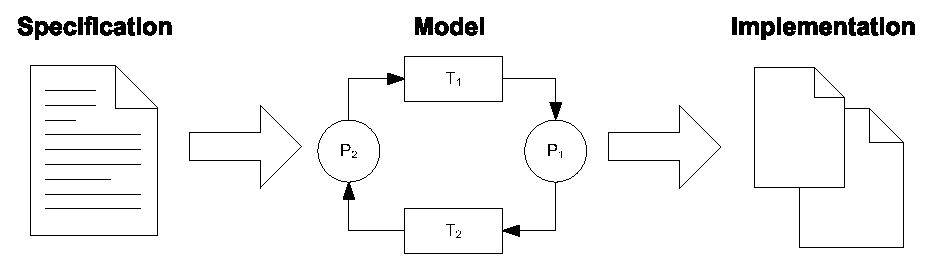
\includegraphics[scale=0.7]{introduction/graphics/spec_model_impl_figure.eps}
\caption{Phases in software development using models}
\label{fig:specmodelimpl}
\end{figure}

%Formal verification advantages
The advantage of constructing a model in the development phase is at least threefold: 
\begin{itemize}
\item Developers are forced to be precise about essential parts of the specification in the process of building the model. Specifications are often ambiguous because they are written in plain English, and details may be missing in the specification. Finding these errors early in the development process can save a lot of resources later.

\item By using the appropriate tools it is possible to perform simulations of a model. A simulation is very similar to an execution of a program. It shows how the model behaves in different situations which can be used to debug the specification. 

\item From a model it is possible to generate a state space, which is a directed graph, where states are represented as nodes and events \ignore{, that changes the system to a new state, }are represented as arcs. The state space can be explored in order to mathematically prove that the system has a given property. This is important in systems were an error can have catastrophic consequences, e.g., in the software controlling the cooling system of a reactive core in a nuclear power plant. 
\end{itemize}

% State space analysis disadvantages
A problem with state space analysis is that the number of states a system can reach often grow rapidly when the model becomes more complex. This is known as the \emph{state explosion problem} \cite{Val98}, and is a big challenge when performing state space exploration. It is often possible to restrict the model, or build the state space partially and still find errors in the system. 

% Translating the model to code
Another problem with the approach shown in Fig.~\ref{fig:specmodelimpl} is that there may be a mismatch between the specification, the model, and the actual implementation. This is because the translation: specification $\rightarrow$ model $\rightarrow$ imhhhplementation is done manually, and hence errors may be introduced in each step of the translation. A way to reduce this problem is to use the model as the specification and automatically generate the implementation from the model. The details abstracted away in the model will of course also lack in the implementation, but eliminating errors in the important parts of the system would lead to more reliable software with fewer errors. \ignore{and could save a lot of resources compared to making the translation manually.}\\

% Example to motivate automatic code generation
Network protocols are an example of why automatic code generation is useful in software development. The \underline{Dy}namic \underline{M}ANET \underline{O}n-demand (DYMO) Routing Protocol \cite{refWorks:69} is a protocol for routing in mobile ad-hoc networks. The Internet Draft describing the protocol is currently at version 16 and about to become an Internet Standard. The specification is written in English describing the different operations of the protocol, and it can be used as a basis for an implementation. Because natural language specifications are often ambiguous translating them to either an implementation or a model requires that the developer make some choices. These choices can make the implementation flawed, and it can also make interoperability between different implementation difficult. 

Specifying DYMO as a formal model (instead of plain English) would exclude ambiguities in the specification. It would also make it easier to directly find errors or verify properties of the specification. In an earlier project \cite{RefWorks:6} we showed, that a model of the DYMO protocol containing all the mandatory parts can be constructed using relatively few resources. The problem is that manually implementing the protocol based on the model may introduce errors, and it would therefore be better \ignore{and more cost-efficient} to generate most of the implementation automatically. In the case of the DYMO protocol, technical details like packet formats and configurations are abstracted away in the model, so they would have to be implemented manually. But the protocol logic and the structure of the implementation would be generated automatically and therefore preserving the behaviour of model in the code.


\section{Coloured Petri Nets}

Petri nets \cite{Petri} is an executable graphical modelling language represented by a bi-graph consisting of nodes and arcs. It can be used to describe a discrete-event concurrent system. An example of such a concurrent system could be a communication protocol. A model could be used to analyse whether it is possible to bring the protocol in an undesirable state, e.g., a deadlock. Nodes in a Petri net are either transitions representing discrete events, or places representing conditions. Arcs in a Petri net describe the pre- and post-condition relation between transitions. 

% Coloured Petri Nets
Coloured Petri Nets (CP-nets or CPNs) \cite{RefWorks:3} is a high-level Petri net language, i.e., the Petri net formalism with added high-level programming functionalities. The programming language used is CPN ML which is based on the general-purpose functional programming language Standard ML \cite{RefWorks:67}. CPN ML provides support for commonly used functionality, e.g., defining data types and manipulating data. Every part of the CPN language has a formal definition, i.e., it is defined mathematically what will happen, e.g., when events occur in the model. This makes it possible to simulate an execution of a CPN model to inspect which states the model can reach. 

CPN Tools \cite{RefWorks:3} is a graphical CPN editor in which it is possible to construct and simulate CPN models. Through the graphical user interface the user can construct a model and do step-by-step simulation. This is much easier than constructing and simulating the CPN model according to the mathematical definition by hand.

When performing a simulation of a model, only one possible execution of the system is explored. But often it is interesting to look at every possible execution of the system to analysis whether it is possible for the model to reach an undesirable state. As mentioned, this can be done by generating and exploring the state space of the model to analyse the behaviour of the system. There exist a range of tools that suppot state space exploration. CPN Tools has built-in support for generating and exploring state spaces. Another computer tool is the \underline{A}SCoVeCo \underline{S}tate space \underline{A}nalysis \underline{P}latform (ASAP) \cite{RefWorks:92}. ASAP is a platform that supports state space analysis of CPN models using state-of-the-art exploration algorithms. The program is built on top of the Eclipse Rich Client platform \cite{RefWorks:73} which makes is very easy to extend, a fact we take advantage of later in this thesis.

\section{Code Generation}
An often used definition of code generation is one computer program producing another computer program in an automatic way. A well known type of code generator is a compiler, e.g., Sun's javac \cite{refWorks:70} or GNU's GCC \cite{refWorks:71}. A compiler typically takes a human-readable text file as input and outputs an executable program. The produced program is often low-level code, e.g., machine code.

The type of code generation presented in this thesis is \emph{source code generation}. The input to this kind of code generator is a formal model specified for instance in a graphical modelling language, and the output is human-readable source code written in a high-level programming language. A compiler has the advantage that high-level programming languages are designed such that the translation into low-level code always makes sense and has equivalent behaviour. Source code generation from a formal model do not have the same advantage. A model is an abstraction of a system and because of the generality of the model it is often very hard to obtain equivalent behaviour in the source code.

Also, the level of abstraction has to be taken into consideration. In one model the focus might be on the details of packet transmission in a network, whereas in another model these details might have been abstracted away. This can make it hard to generate code since it is difficult to make an interpretation of the structures in the model.

\section{Thesis Aims and Results}
The aim of this thesis is to develop a technique to automatically generate code from CPN models. The code should be readable and intuitive such that the user can read, modify and extend the generated code. We also require that the model should be clearly recognizable in the generated code since the people working with the generated code would typically be very familiar with the model. The technique should allow different target languages to be used, e.g., C, Java, SML or Erlang. However the target language should be invisible in the model and the usual inscription language should be used in the model.

We achieved the aim by defining a subclass of CP-nets called Process-Partitioned CP-nets (ProPCP-nets or ProPCPNs). ProPCPN models preserve most of the general-purpose strength of CP-nets as we show by constructing a model of the advanced DYMO protocol. We have developed a technique that translates from the class of ProPCP-nets to the Erlang programming language, and created an implementation of the technique as a proof of concept. The implementation is able to generate readable code from the DYMO model, and we validate that the generated code has the same behaviour as the model. 


\ignore{
%% OLD AIM:
%% Model: Restriction vs. expressiveness, target language invisible
Our aim is to define a subclass of CP-nets which preserves the general-purpose strength of CP-nets, but enables us to generate code for the models in the class. To show the expressive power of the class we construct a model of the complex communication protocol DYMO in this class. Our focus in the translation is more on generating readable code than on generating high performance code. It is for instance more important that the programmer is able to recognize the model in the code than making the code highly optimised.

%% Tool
As a proof of concept we implement a tool which given a CPN model in our subclass of CPNs generates an Erlang source code implementation of the model. The implementation should have the same behaviour and properties as the model.

}

\section{Thesis Outline}
The structure of the thesis is described below. The thesis is written in close cooperation between the two authors, but as required we have divided the responsibility of the chapters. 

\begin{description}
\item[Chapter~\ref{chap:background}~\nameref{chap:background}] In this chapter we establish the background for understanding the thesis. We present the CPN model of a producer-consumer system which is the running example throughout the thesis. We also present the target language of the translation, namely Erlang, and describe the basic constructs of the Erlang language. Kristian is responsible for Sec.~\ref{sec:cpn}, and Mads is responsible for Sec.~\ref{sec:erlang}. 

\item[Chapter~\ref{chap:codegeneration}~\nameref{chap:codegeneration}] Different approaches to code generation is discussed on the basis of related work. We illustrate some of the approaches using manually translated code examples, and discuss advantages and disadvantages. Mads is responsible for this chapter.

\item[Chapter~\ref{chap:netclass}~\nameref{chap:netclass}] ProPCPN is a subclass of CPN that we constructed to generate code from, and we give an intuitive description as well as a formal definition of the net class. We also show that the producer-consumer model presented in chapter~\ref{chap:background} fits into this subclass. Mads is responsible for this chapter.

\item[Chapter~\ref{chap:translation}~\nameref{chap:translation}] In this chapter we present a technique to generate Erlang source code from ProPCPN models. We present all the phases of the translation, and use the simple producer-consumer model to illustrate the translation. Mads is responsible Sec.~\ref{sec:cpntodcpn}, Sec.~\ref{sec:dcpntocfg}, and Sec.~\ref{sec:cfgtoast}. Kristian is responsible for Sec.~\ref{sec:astest}, Sec.~\ref{sec:esttocode}, and Sec.~\ref{sec:advancedissues}.

\item[Chapter~\ref{chap:tool}~\nameref{chap:tool}] In this chapter we present our implementation of the translation technique presented in chapter~\ref{chap:translation}. We also validate the code generated from the producer-consumer model. Kristian is responsible for this chapter.

\item[Chapter~\ref{chap:dymo}~\nameref{chap:dymo}] In this chapter we show the expressive power of ProPCPN models by constructing a model of the industrial-sized protocol DYMO. We automatically generate code from the model using our implementation of the translation, and show that the protocol logic from the model is preserved in the generated code. Kristian is responsible for this chapter.

\item[Chapter~\ref{chap:confutwo}~\nameref{chap:confutwo}] Finally, we conclude and summaries on the findings in this thesis and outline some directions for future work.

\end{description}

The implementation of the translation can be found on the enclosed CD-ROM (see appendix \ref{appsec:cd} for more information). The reader is expected to have a basic understanding of formal models, whereas the formal modelling language Coloured Petri Nets is introduced in section \ref{sec:cpn}. Knowledge about SML (or a similar functional language) is also expected, whereas the fundamental concepts of the functional programming language Erlang are explained in section~\ref{sec:erlang}.

\chapter{CP-nets and the Erlang Language}
\label{chap:background}

In this chapter we present the formal modelling language Coloured Petri Nets and the functional programming language Erlang. A basic understanding of these topics is required to understand the rest of the thesis.

\section{Coloured Petri Nets}
\label{sec:cpn}
One way to approach the challenge of building concurrent systems is to build a formal model, e.g., a Coloured Petri Net (CPN) \cite{RefWorks:3} model. Constructing and simulating an executable model gives insight into the system being modelled and reveals errors. Furthermore, building the model often leads to a more complete specification. A CPN model of a system describes the state and the events that can change the state of the system. The model can be simulated which enables the developer to investigate the system through different scenarios.

% Producer-consuming example description
We explain the CPN language through a producer-consumer system which will be the running example throughout this thesis. In our producer-consumer system two different kinds of entities are running concurrently:	

\begin{itemize}
  \item $n$ producers run simultaneously. A producer alternates between producing and sending data to a consumer. 
  \item $m$ consumers run simultaneously. A consumer alternates between receiving data from a producer and consuming data.  
\end{itemize} 

The data produced, send, received, and consumed is represented as integers. Producers can send the produced data to a specific consumer determined by the value of a global variable. In section~\ref{sec:validateprodcons} we introduce a load-balancer which can change the value of this global variable.

\begin{figure}[b!]
\centering
\includegraphics[scale=0.5]{background/graphics/System.eps}
\caption{The producer-consumer CPN model}
\label{fig:systemmodule}
\end{figure}

% The producer-consumer CPN model
A graphical drawing of the CPN model is shown in Fig. \ref{fig:systemmodule}. The top part models the producers and the bottom part models the consumers. The CPN model contains nine \emph{places} (drawn as ellipses), four \emph{transitions} (drawn as rectangular boxes), a number of directed \emph{arcs} connecting places and transitions, and finally some textual \emph{inscriptions} next to the places, transitions and arcs. The inscriptions are written in an extension of the Standard ML language called \emph{CPN ML}. Places and transitions are called \emph{nodes} and together with the arcs they constitutes the \emph{net structure}. An arc either connects a transition to a place or a place to a transition. Thus it is illegal to, e.g., connect a place to another place.  

% Places
The places represent the state of the modelled system. Each place has a number (possibly zero) of tokens, and each token has a data value (called a \emph{token colour}) attached to it. The \emph{marking} of a specific place is the number of tokens and their colour on that place. The marking of the entire CPN model is described by the union of the markings of each place in the model. The state of the producers is described by the four places \figitem{Producing}, \figitem{Sending}, \figitem{Data}, and \figitem{ProducedData}. The state of the consumers is described by the three places \figitem{Receiving}, \figitem{Consuming} and \figitem{ReceivedData}. 

Each place has a type inscription, called the \emph{colour set}, that specifies which token colours are allowed on that place. The colour set keyword in CPN ML is simply \code{colset}. The colour set at the places \figitem{Producing} and \figitem{Sending} is \code{PRODUCER}, and the colour set at the places \figitem{Receiving} and \figitem{Consuming} is \code{CONSUMER}, which are defined:

\begin{verbatim}
colset PRODUCER = index p with 1..2;
colset CONSUMER = index c with 1..2;
\end{verbatim}

\noindent
Both \code{PRODUCER} and \code{CONSUMER} are \emph{index} colour sets. Indexed values are sequences of values comprised of an identifier and an index-specifier. These colour sets are used to represent and identify the different producers and consumers. The places \figitem{Data} and \figitem{ProducedData} have the colour set:

\begin{verbatim}
colset PRODUCERxDATA = product PRODUCER * DATA; 
colset CONSUMERxDATA = product CONSUMER * DATA;
\end{verbatim}

\noindent
The \code{product} keyword is used to create tuples. Both \code{PRODUCERxDATA} and \code{CONSUMERxDATA} are two-tuples (pairs) where the first element is a producer or a consumer respectively and the second element is data.

Next to each place there is another inscription called the \emph{initial} marking. For instance, the place \figitem{Producing} has the initial marking \code{PRODUCER.all()} which specifies that the initial marking of \figitem{Producing} contains all producers. Analogously, the place \figitem{Receiving} contains all the consumers initially. The number of producers and consumers depends on the scenario investigated. In this example we have two producers and two consumers. The initial marking of the place \figitem{Data} is described by the multi-set:

\begin{verbatim}
1`(p(1), 1) ++ 1`(p(2), 2);
\end{verbatim}

\noindent
A \emph{multi-set} is a set where elements are quantified. The \code{++} and \code{`} are operators on multi-sets. The elements are quantified by the infix operator \code{`} which takes a non-negative integer as left argument and an element as right argument. For instance, \code{1`(p(1), 1)} means that there is one appearance of the element \code{(p(1), 1)}. The meaning of the pair \code{(p(1), 1)} is that we associate producer \emph{1} with the integer data element one. The multi-set infix operator \code{++} is used to take the union of two multi-sets. The places \figitem{Sending}, \figitem{ProducedData}, \figitem{Consuming} \figitem{ReceivedData} and  \figitem{Buffer} are initially empty, whereas the place \figitem{NextConsumer} contains the multi-set \code{1`c(1)}.

% Transitions 
The four transitions (drawn as rectangles) represent the events that can occur in the system. When a transition \emph{occurs} it removes tokens from \emph{input} places (those having an arc pointing towards the transition) and adds tokens to the \emph{output} places (those having arcs pointing away from the transition). For instance, when the transition \figitem{ProduceData} occurs it removes a producer token from the input place \figitem{Producing} and a data token, belonging to the same producer, from the input place \figitem{Data}. Then it adds the same producer token to the output place \figitem{Sending} and the pair associating the producer with the data to the output place \figitem{ProducedData}. 

% Arcs
The colour of a token added or removed by a transition is determined by the \emph{arc expressions} on the arcs connecting the transition to the input and output places. The arc expressions are written in the CPN ML programming language and may contain constants, typed variables, operator expressions or functions. The arc expressions are evaluated when all variables are bound to a value and evaluates to a multi-set of token colours. On an output arc the multi-set of token colours outputted by the arc expression is added to the connected output place. On an input arc the multi-set of token colours outputted by the arc expression is removed from the connected input place. As an example, consider the two arcs connecting the input places \figitem{Producing} and \figitem{Data} to the transition \figitem{ProduceData}. The two arc expressions contain the variables: 

\begin{verbatim}
var prod : PRODUCER
var data : DATA
\end{verbatim}

\noindent
This means that \code{prod} must be bound to a value of type \code{PRODUCER} and data must be bound to a value of type \code{DATA}. A valid \emph{binding} of variables could be the following binding which binds \code{prod} to producer \emph{1} and \code{data} to the integer one:

\begin{verbatim}
<prod=p(1),data=1>
\end{verbatim}


\subsection{Enabling and Occurrence of Transitions}
A transition is \emph{enabled} if the arc expressions on the \emph{input} arcs evaluates to multi-sets which is present on the input places connected to the transitions. Furthermore, the guard of the transition must evaluate to \emph{true} (guards are explained in section \ref{subsec:guards}). We then say that the transition can \emph{occur} in that marking. When the transition occurs it removes from each input place the multi-set of token colours to which the corresponding input arc evaluates. It then adds to each output place the token colours to which the corresponding output arcs evaluate.

\begin{figure}
\centering
\includegraphics[scale=0.40]{background/graphics/SystemProducerM0.eps}
\caption{The initial marking $M_0$ showing the producer part of the model}
\label{fig:systemmoduleProducerM0}
\end{figure}

Let us consider Fig.~\ref{fig:systemmoduleProducerM0} in which the initial marking of the producer part of the model are shown. We see two producers on the place \figitem{Producing}. Producer \code{p(1)} has the integer data value \code{1} on the place \figitem{Data} and producer \code{p(2)} has the value \code{2}. The transition \figitem{ProduceData} has a thick border line which in CPN Tools means that the transition is enabled. The transition \figitem{SendData} is not enabled meaning it can not occur in the initial marking. There are two possible bindings for the variable \code{prod} on the input arc going from the input place \figitem{Producing} to the transition \figitem{ProduceData}. If \code{prod} is bound to \code{p(1)} the task is to find a binding of the variables on the input arc connecting the \figitem{Data} to \figitem{ProduceData} such that the arc expression evaluates to a multi-set of tokens where \code{prod=p(1)}. The resulting binding is:

\begin{verbatim}
<prod=p(1),data=1>
\end{verbatim}

\noindent
An occurrence of the transition \figitem{ProduceData} with the binding from above removes the token with colour \code{p(1)} from \figitem{Producing} and \code{(p(1),1)} from \figitem{Data}. It then adds the result of evaluating the output arc expressions, which means that a token colour \code{p(1)} is added to the place \figitem{Sending}, the pair \code{(p(1),1)} is added to the place \figitem{ProducedData} and the pair \code{(p(1),3)} is added to the place \figitem{Data}. The resulting marking $M_1$ is shown in Fig. \ref{fig:systemmoduleProducerM1} and again only the producer part of the model is shown since the marking of the consumer part is unchanged. 

\begin{figure}[b!]
\centering
\includegraphics[scale=0.40]{background/graphics/SystemProducerM1.eps}
\caption{The producer part of the model in marking $M_1$}
\label{fig:systemmoduleProducerM1}
\end{figure}

In marking $M_1$ in Fig.~\ref{fig:systemmoduleProducerM1} we can see that the token colour \code{p(1)} now resides on the place \figitem{Sending} and that the transition \figitem{SendData} now has a thick border line indicating that it is enabled. Intuitively, this means that the producer \emph{1} is now in a sending state ready to send out the data that was just produced. 

The notation for the occurrence of a transition with a given binding is called a \emph{binding element} and is written as a pair where the first element is the transition and the second element is the binding of variables for that transition. In the marking $M_1$ there are two binding elements enabled: \\*
\newline
(\figitem{ProduceData}, \code{<prod=p(2),data=1>})\\*
(\figitem{SendData}, \code{<prod=p(1),data=1, nextcons=c(1)>})\\*
\newline
Choosing the second binding element results in adding a data element to the buffer and changing the state of producer \emph{1} back to producing. Letting this binding element occur will lead to marking $M_2$ which can be seen in Fig.~\ref{fig:systemmoduleM2}. In this marking the token \code{p(1)} is moved back to the place \figitem{Producing} and the token \code{c(1),1} is added to the place \figitem{Buffer}. This means that data can now be received by a consumer \emph{1}. Notice how the variable \code{nextcons} is used to determine the receiver of the produced data. In a sense, the place \figitem{NextConsumer} is trivial representation of a \emph{load-balancer} that never changes the receiver of the produced data. In section~\ref{sec:validateprodcons} we present a more useful load-balancer. 

\begin{figure}
\centering
\includegraphics[scale=0.35]{background/graphics/SystemM2.eps}
\caption{The marking $M_2$ after the occurrence of \figitem{SendData}}
\label{fig:systemmoduleM2}
\end{figure}

\subsection{Concurrency and Conflict}
Two binding elements are in conflict if they are both enabled, but the occurrence of one of them removes a token also needed by the other binding element. In the marking $M_2$ there are three binding elements enabled: \\*
\newline
$PD_1$ = (\figitem{ProduceData}, \code{<prod=p(1),data=3>})\\*
$PD_2$ = (\figitem{ProduceData}, \code{<prod=p(2),data=1>})\\*
$SD_1$ = (\figitem{SendData}, \code{<cons=c(1),data=1>})\\*
\newline
The first two binding elements represent a producer producing some data and the last binding element represents a consumer receiving some data. All these binding elements can occur \emph{concurrently}, i.e., in parallel, thus there are no conflicts here. The producer and consumer runs concurrently since two binding elements, where one of the binding elements include a transition from the producer part of the model and the other binding element includes a transition from the consumer part of the model, are never in conflict. This is because no places in the model are input places for both transitions in the producer and consumer part of the model. 

The occurrence of binding element $SD_1$ leads to the marking $M_3$ shown in Fig. \ref{fig:systemmoduleConsumerM3}. The data item has been removed from the buffer and the transition \figitem{ReceiveData} is no longer enabled as explained above. The consumer \emph{1} is now ready to consume the received data.

\begin{figure}[b!]
\centering
\includegraphics[scale=0.4]{background/graphics/SystemConsumerM3.eps}
\caption{The consumer part of the model in marking $M_3$}
\label{fig:systemmoduleConsumerM3}
\end{figure}


\subsection{Guards}
\label{subsec:guards}
Transitions are also allowed to have a guard which is a list of boolean expressions. A transition is only enabled if the guard expression evaluates to \emph{true} in the binding, thus putting an additional constraint on the transition. As an example of a guard consider the modified transition \figitem{ReceiveData} in Fig. \ref{fig:partsystemwithguard}. The guard of the transition \figitem{ReceiveData} is the boolean expression in the square brackets. It ensures that \code{c(1)} only receives even integers, whereas other consumers can receive both odd and even integers. This is done by first checking whether the \code{cons} variable is bound to the value \code{c(1)} and if so whether the variable \code{data} is bound to an even integer. \code{true} is returned for other values of the \code{cons} variable indicating no constraint on the enabling of the transition for these consumers.

\begin{figure}
\centering
\includegraphics[scale=0.35]{background/graphics/PartSystemWithGuard.eps}
\caption{A guard constraining the enabling of the transition \figitem{ReceiveData}}
\label{fig:partsystemwithguard}
\end{figure}


\section{The Erlang Language}
\label{sec:erlang}
Erlang -- named after the Danish mathematician Agner Krarup Erlang (1878-1929)~\cite{RefWorks:76} -- is a concurrent message-oriented functional programming language. In order to understand Erlang it is helpful to first understand the history of Erlang. The following is built on the experience of Joe Armstrong - one of the creators of Erlang \cite{RefWorks:75}. The Erlang language was a result of research done by Ericsson in the 1980's. The overall goal for Ericsson was to have a language that was suitable for programming large telephone switches, i.e., could handle a lot of concurrent phone calls and establish connections within a few milliseconds. It started out as a dialect of Prolog in 1987, but in 1990 the Erlang language was born with its own syntax, virtual machine, and function libraries.

In the early nineties Erlang was used in product development at Ericsson and in 1993 the first commercial version was released. In 1998 a very large project was finished with the AXD301 ATM (Asynchronous Transfer Mode) switch used by, e.g., the British Telecom. The software on the AXD301 consists of 2.6 million lines of code which is very large for a functional language. The AXD301 is extremely reliable (the measured reliability is a down time of 31 ms per year) and each node can handle millions of calls per day. The same year Ericsson decided to discontinue the development of Erlang due to changes in business strategy and made Erlang open source and free to download~\cite{RefWorks:76}. 

A recent example of the use of Erlang in a larger projects is the chat system on Facebook \cite{Facebook,RefWorks:81} which can handle millions concurrent users. The chat system is an example of how Erlang can be used in the parts of a system where Erlang has its advantages, while leaving other parts to more fitted programming languages. For instance the user interface of the chat system is written in PHP/JavaScript and the logging of messages in C++. 

\subsection{Language Overview}
The original intention for Erlang has made an impact on the language today \cite{RefWorks:76,RefWorks:77}. Erlang is a highly concurrent programming language and basically everything is a process. There is no shared memory between processes, and hence all communication is done by asynchronous message passing placing Erlang in the class of \emph{Message-oriented} languages. This eliminates many errors since a process can be implemented in isolation without sharing resources with other processes. In order to handle millions of processes they must be very lightweight, i.e., require little memory, have fast loading/destroying times and message passing must require little computational effort. Studies show \cite{RefWorks:74} that processes in Erlang are indeed lightweight, and that hundreds of thousands of processes can be handled without noticeably degrading the performance of the system. 

Because Erlang builds on the functional programming paradigm there is no mutable data. The absence of side-effects makes it easier to verify program correctness and also to parallelise the program. Some features from other functional programming languages are left out to keep the language simple and efficient. Currying is for instance not a feature in Erlang. 

Erlang is designed to run on reactive (non-stop) systems, e.g. an air traffic control system, and it is therefore possible to update Erlang software without shutting down the system. It is always possible to use the newest version of the software since a function call with a qualified name is dynamically linked in the run-time code. Changing the version of modules can be done by parsing a message to the process.

Compared to Standard ML, Erlang has a more dynamic type system. This means that some errors are only caught on runtime, e.g. a match operation may fail or a BIF (Build-In Function) may be evaluated with an illegal argument. It is possible though to create fault-tolerant programs by using mechanisms provided by Erlang to detect and handle such errors. Catch and throw constructs provide a mechanism for monitoring the evaluation of an expression. Another mechanism called \emph{linked processes} can be used to have a process monitor the behaviour of another process. If a process terminates (normally or abnormally) a signal is sent to all the linked processes together with a reason for the exit. The linked process can then act on this, e.g., try to recover from the error or terminate.

\subsection{The Producer-Consumer System in Erlang}
\label{sec:producerconsumererlang}

In this section we explain the basics of Erlang through the simple
producer-consumer system explained in section \ref{sec:cpn}. The setup
is two producer processes sending messages to two consumer
processes. The producers are informed which consumer to send data to
by reading the value of a shared store called "next\_consumer". A
shared store can only be accessed by one process at a time, i.e., the
store becomes locked when is it read and unlocked when it is written
to. Because of this interaction pattern it is important that when a
process access the store it always first reads the value and then
writes a (possibly the same) value back to the variable. This locking
mechanism is introduced to make it possible to, e.g., add one the
current value of the store.

In order to interact with such a shared process we have made a small
and very simple protocol. A process wanting to read the value of the
store sends the pair \code{\{get, Id\}}, where \code{get} is the atom
we have chosen for the read command and \code{Id} is the process
identifier of the sending process. The shared store will then become
locked and sends the value it contains back to the process. A process
writes a value to the store by sending the pair \code{\{set, Exp\}},
where \code{set} is the atom we have chosen for the write command and
\code{Exp} is some expression. The shared store will then become
unlocked and contain the value that \code{Exp} evaluates to.

\subsubsection{The Producer}

The basic unit of Erlang code is \emph{modules} containing attributes
and function declarations. A module must be stored in a \code{.erl}
file which can be compiled into a binary \code{.beam} file and
executed on the virtual machine. The module that contains the code for
the producer part of the producer-consumer system can be seen in
Listing~\ref{fig:erlangproducer}.


\begin{figure}
\label{fig:erlangproducer}
\begin{verbatim}
-module(producer).
-export([produce/1]).

produce(Data) ->
  Produced_data = Data + 2,
  io:format("Producing data ~w.~n", [Produced_data]),
  next_consumer ! {get, self()},
  receive 
    Nextcons -> 
      Consumer_ID = list_to_atom("consumer_ID" ++
      integer_to_list(Nextcons)),
      Consumer_ID ! Produced_data,
      next_consumer ! {set, Nextcons}
  end,
  timer:sleep(2000),
  produce(Produced_data).
}
\end{verbatim}
\end{figure}


The \emph{module declaration} is the only mandatory attribute declaration and in line 1 we see the declaration. A period (.) is used after each attribute and function declaration to separate them from one another. In line 2 we find the \emph{export declaration} that can be used to make functions visible to other modules. The functions are specified in a list on the form \emph{function\_name} / \emph{number\_of\_arguments}. These function can then be accessed by using the syntax \emph{module\_name}:\emph{function\_name} from outside the module. In this case the \code{produce} function taking one argument is the only function exported.

The module defines the function \code{produce}. A function is a sequence of clauses separated by semicolons (;) and terminated by a period (.). The function \code{produce} is defined in line 4 through 16 and has only a single clause. As we can see Erlang do not use any keyword for defining functions. To define a function, the name of the function is stated followed by the arguments in parenthesis. In this case the function \code{produce} takes one argument \code{Data}. The name of the function together with the arguments is called the clause head. It is followed by the symbol "\code{->}" and then the clause body where the expressions of the clause are defined (separated by comma (,)).

In Erlang \emph{atoms} are used to represent non-numerical constant values and are very similar to enumerated types in for instance C or Java. An atom either begins with a lowercase letter or is put into single quotation marks ('). The name of a function must be an atom, e.g., the function name \code{start} is an atom. We can also notice that the arguments begin with an uppercase letter. The arguments are essentially variables and in Erlang all variables must begin with an uppercase letter.

In line 4 we see the atom \code{produce} and the \emph{clause head} \code{producer (Data)} followed by the symbol \code{->} which indicates that the \emph{clause body} is about to start. In line 5 we find the first expression on the right hand side of the "=" operator, namely \code{Data + 2}. On the left hand side we find the new variable \code{Produced\_data}. Notice that "=" is not an assignment operator in Erlang but a \emph{pattern matching} operator. Thus in line 5 the value of the expression on the right hand side is matched to the expression on the left hand side, i.e., a single variable. This results in the value of the right hand side being assigned to the variable \code{Produced\_data}. In Erlang a variable can either be \emph{bound} or \emph{unbound}. A bound variable cannot get a new value assigned to it which is known as \emph{single assignment variables}.

In line 6 we encounter the first use of a \emph{built-in function} (BIF). The function \code{format} in the \code{io} module can be used to print text to the screen. \code{format} takes as arguments the string to be printed and a list of \emph{terms}. In Erlang terms is a piece of data of any type. The \verb|~w| in the string is substituted by the terms in the list in turn and the string is ended by the new line character \verb|~n|.

In line 7 the producer sends the pair \code{\{get, self()\}} to the shared store process registered under the name \code{next\_consumer}, using message passing. In Erlang tuples are a compound data type with a fixed number of elements. It is defined using curly brackets "\{" and "\}" as in line 7. The send operator, which is an exclamation mark (!), is used to send the messages to the shared store. The left hand side of the operator specifies the process that should receive the message, and on the right hand side the message to be sent. As we can see in line 7 the \code{producer} process is sending the tuple to a process called \code{next\_consumer}.

The atom \code{get} in the messages tells the shared store that the process wants to receive the data the shared store contains. The BIF function \code{self()} returns the process identifier of the currents process. Sending the process identifier enables the shared store to send the value back to the messages that requested it. The atom \code{get} also locks the shared store such that other processes cannot changes the value before this process sends a \code{set} message back.

Line 8 contains the Erlang keyword \emph{receive} that starts a \emph{receive expression}. Making a receive expression allows a process to receive the messages which have been sent by other processes to this process. A receive expression has a number of patterns which is matched against the incoming message and the body of the first pattern that matches is evaluated. The current process is blocked until a message that matches one of the patterns has been received. The receive expression in the \code{produce} function only has a single pattern. This pattern consists of the unbound variable \code{Nextcons} (seen in line 9) which becomes bound when the message is received. An unbound variable matches all expression which means that the producer process is ready to receive the data sent from the shared store.

In line 10 and 11 the identifier of the consumer process is constructed. These two lines construct an atom containing first \code{consumer\_ID} followed by the identifier received from the shared store. The way this is done is by using the BIF \code{integer\_to\_list} to turn the received identifier into a list. In Erlang there are no strings which means that \code{"consumer\_ID"} is actually a list of integers. The two lists are concatenated using the list operator \code{++}. The resulting list is converted into an atom using the BIF \code{list\_to\_atom}.

In line 12 the produced data is sent to the consumer using the constructed identifier from line 10 and 11. In line 13 the pair \code{\{set, Nextcons\}} is sent to the shared store to unlock it, thus making the value available to other processes. The receive expression is ended in line 14 by the keyword \code{end}.

The process is put to sleep for 2000 milliseconds in line 15. This is done by using the BIF \code{sleep} in the module \code{timer}. Finally in, line 16 the \code{producer} function makes a recursive call to itself with the argument \code{Produced\_data}, i.e., the value of \code{Data} increased by two. It is important to notice that the last function call in the sequence of expressions in the clause body is the recursive call. This is known as \emph{tail-recursion}. Using tail-recursion allows the compiler to replace the function call with a jump to the start of the function, and hence the execution stack will not be filled with return addresses. So the result is a function that will loop forever.

\subsubsection{The Consumer}
The module that holds the code for the consumer part of the producer-consumer system can be seen in Listing~\ref{fig:erlangconsumer}. The first two lines are very similar to those of Listings~\ref{fig:erlangproducer}. First, we see the module declaration that declares the name of the module followed be the export declaration which states that the function \code{consume} with no arguments should be visible from outside the module.

\begin{figure}[h!]
\begin{verbatim}
-module(consumer).
-export([consume/0]).

consume() ->
  receive
    Data ->
      io:format("Consuming data ~w.~n", [Data]),
      consume()
  end.
\end{verbatim}
\end{figure}

Line 4 through 9 defines the \code{consume} function. First, we see the clause head consisting of the atom \code{consume} and an empty list of arguments. Following the symbol "\code{->}" we see the clause body which begins (in line 5) with a receive expression. This receive expression has a single pattern which consists of an unbound variable \code{Data} that becomes bound when the message is received. This means that the consumer process is ready to receive any kind of data that must be sent to it.

In line 7, the BIF \code{format} is used to print the received data to the screen. In line 8, the function makes a recursive call to put the process in a state ready to receive a new message. Again, the last function call in the sequence of expressions is the recursive call which means that this function also uses tail-recursion. Finally, in line 9 the receive expression is ended with the keyword \emph{end}. 

\subsubsection{The Shared Store}
\label{subsec:thesharedstore}
The shared store can be viewed as a global variable which can be accessed by any running Erlang process. In Listing~\ref{fig:erlangshared} is shown the implementation of the module \code{shared} which has the behaviour of a shared store. At the top of the module we find the module declaration and the export declaration that exports the \code{start} function. The \code{start} function takes one argument, namely the initial value of the store. The \code{handle\_request} function takes one argument which is the current value of the shared store.

\begin{figure}[h!]
\begin{verbatim}
- module(shared).
- export([start/1]).

start(Init_value) -> 
  handle_request(Init_value).

handle_request(Value) -> 
  receive 
    {get, Id} -> 
	  Id ! Value
  end,
  receive 
    {set, New_value} -> 
	  handle_request(New_value)
  end.
\end{verbatim}
\end{figure}

The function \code{handle\_request} contains two receive expressions. The first blocks the process until it receives a pair containing the atom \code{get} and a process identifier. It then sends \code{Value} back to the requesting process. The process then moves on to the next receive expression where it is blocked (locked) until it receives a pair containing the atom \code{set} and a value \code{New\_value}. A recursive call is then made with \code{New\_value} as argument, which then becomes the new value of the shared store. The recursive call also unlocks the store and it is ready to receive a new \code{get} request.

\subsubsection{Register and Spawn Processes}

We need a process that starts the \code{producer}, the \code{consumer}, and the \code{shared} processes, in order to get the producer-consumer system running. In Listing~\ref{fig:erlangsystem} we find the \code{system} module doing exactly this. The \code{start} function is defined in line 4 through 9. The BIF function \code{spawn} creates a new process and returns the process identifier (pid) that has been assigned to that process. \code{spawn} takes as arguments the module name, the name of the function that starts the process, and a list of arguments to that function. In line 5 \code{spawn} is called with the module \code{shared}, the function \code{start} and an empty list because the function \code{start} in the module \code{shared} takes on arguments.

\begin{figure}[h!]
\begin{verbatim}[style=erlangcode, caption=The module system.erl, label=fig:erlangsystem]
-module(system).
-export([start/0]).

start() ->
  register(next_consumer, spawn(shared, start, [1])),
  register(consumer_ID1, spawn(consumer, consume, [])),
  register(consumer_ID2, spawn(consumer, consume, [])),
  spawn(producer, produce, [1]),
  spawn(producer, produce, [2]).
\end{verbatim}
\end{figure}

In line 5 we also see the use of the BIF \code{register}. This function is used to register processes under symbolic names. The function takes as argument an atom which is the symbolic name of the process and the pid of the process. In our case we register the newly spawned \code{shared} process under the symbolic name "next\_consumer". This enables the \code{producer} processes to send messages to the \code{next\_consumer} process without knowing the pid of the shared store.

In line 6 through 9 two \code{producer} processes and two \code{consumer} processes are spawned using the \code{spawn} function. The \code{consumer} processes are started by calling the function \code{consume} with no arguments. The \code{producer} processes are started by calling the function \code{produce} given the arguments 1 and 2 respectively.

\subsubsection{The Record Data Structure}
The data structure \emph{record} could be used in the producer-consumer system to represent a message. A record definition consists of an atom which is the name of the record. This is followed by a tuple of atoms which defines the field names of the record. The definition of a \code{message} record can be seen in Listings~\ref{fig:erlangmessage}.

\begin{figure}[h!]
\begin{verbatim}
-record (message, {
	id,
	data
	}).
...

Msg = #message{id = self(), data = 1}
\end{verbatim}
\end{figure}


In lines 1-4, the \code{message} record with two field are defined, namely \code{id} and \code{data}. In line 7 of the pattern matching operator is used with a new variable \code{Msg} on the left hand side. On the right hand side we see the notation for creating a new record. The first field named \code{id} is assigned the pid of the current process and the second field named \code{data} is assigned the value 1.



\chapter{Approach to Code~Generation}
\label{chap:codegeneration}
There are different approaches to automatically generate code from Petri nets, and the chosen strategy has a large impact on the properties of the final code. The approach should preserve the behaviour of the model, but the code generated in one approach might be very efficient, while the code in another approach may be very readable and extensible.

In this section the approaches on code generation from Petri nets are, based on the descriptions in \cite{RefWorks:4} and \cite{RefWorks:5}, divided into the four categories \emph{simulation-based}, \emph{structural-based}, \emph{state space-based} and \emph{decentralised approach}. In each approach we discuss related work, and for the \emph{structural based} and \emph{state space based} approaches we present Erlang code for the producer-consumer system as it would be generated in these approaches. These examples are used as a basis of the discussion of advantages and disadvantages, and to give a better understanding, of the two approaches. The generated code in both examples preserve the behaviour of the model, but are very different in programming style.

\section{Simulation-based Code Generation}
The basic idea in the simulation-based approach is to have a central component which controls the flow of the program on the basis of the state of the environment. This is done by a scheduler which given the current state of the system computes which state to proceed to. The process of determining which state to proceed to corresponds to finding an enabled transition in the CPN model.

The simulation-based approach is used by Philippi \cite{RefWorks:4} to generate Java code from a high-level Petri net. The idea is to make a class diagram which outlines the classes and method signatures of the program. From this diagram, classes with attribute definitions and methods with empty bodies are generated. The empty bodies are filled with the simulator code made from the formal model. After this, the structure of the Petri net is used to enhance the code to make it more efficient and more readable. The simulation-based approach is also used in the projects described in \cite{RefWorks:78} and \cite{RefWorks:2}. In the Course of Action Scheduling Tool (COAST) project \cite{RefWorks:2} the generated simulator code made from a CPN model (by CPN Tools) was used directly in the final implementation. The code was used for scheduling resources and planning of tasks. A similar approach was taken in the project \cite{RefWorks:78} which considered an access control system. This project made use of a simulation kernel generated by Design/CPN \cite{DESIGNCPN}, the predecessor of CPN Tools. The simulation kernel was generated on basis of a CPN model and after undergoing some automatic modifications, e.g., linking the code to external code libraries and changing the dialect of the language, the generated code was embedded into the final implementation of the control unit of the system.

\subsection{Simulation-based Producer-Consumer System}
In this section we describe how the producer-consumer model can be translated into the Erlang programming language using the simulation-based code generation approach. The producer and the consumer part of the model have been identified and leads to two different modules each of them containing a scheduler. The scheduler is an Erlang function that on the basis of a \emph{state id} (sid) decides which function is to be invoked next. This decision resembles computing enablings in a CPN model.

An Erlang module \code{system} (see Listing \ref{fig:simulationsystem}) is responsible for starting up \code{producer} and \code{consumer} processes, and a process to handle the shared store called \code{shared}. The \code{system} module has a single function called \code{start} which first spawns the shared store process \code{next\_consumer}. Next, two \code{consumer} processes are spawned and registered under the names "consumer\_ID1" and "consumer\_ID2" and analogously for two \code{producer} processes. This corresponds to the scenario from the CPN model described in section~\ref{sec:cpn}. All processes can now use this symbolic name to pass messages to other processes.

%\lstset{language=erlang}
\begin{figure}[h!]
\begin{verbatim}
- module(system).
- export([start/0]).

start() -> 
  register(next_consumer, spawn(shared, start, [1])),
  register(consumer_ID1,
           spawn(consumer, start, [undefined])),
  register(consumer_ID2,
           spawn(consumer, start, [undefined])),
  register(producer_ID1,
           spawn(producer, start, [undefined, 1])),
  register(producer_ID2,
           spawn(producer, start, [undefined, 2])).
\end{verbatim}
\end{figure}




The module \code{shared} that implements a shared store is identical to the one presented in section~\ref{sec:erlang}. Processes can read the value of the store by sending a \code{get} messages along with a process identifier. Processes can also set the value of the shared store by sending a \code{set} message along with a value.

\paragraph{The producer part}
Listing~\ref{fig:simulationproducer} shows the manually translated Erlang code for the producer part of the producer-consumer CPN model. The Erlang module has a function named \code{start} that initialises the environment with the values given as arguments and calls the scheduler \code{producer\_scheduler} with the environment and the id of the initial state which is \code{producing}. The scheduler then chooses which function should be called given the state \code{Sid}.

%\lstset{language=erlang}

\begin{verbatim}
-module(producer).
-export([start/2]).
-record(environment, {
    data,
    produced_data
  }).

start(Produced_data, Data) ->
  Env = #environment{data = Data,
  produced_data = Produced_data},
  producer_scheduler(producing, Env).

producer_scheduler(Sid, Env) ->
  {NewSid, NewEnv} = case Sid of
    producing ->
      produce_data(Env);
    sending ->
      send_data(Env)
  end,
  producer_scheduler(NewSid, NewEnv).

produce_data(Env) ->
  Data = Env#environment.data,
  NewEnv = Env#environment{data = Data + 2,
  produced_data = Data},
  {sending, NewEnv}.
  
send_data(Env) ->
  Data = Env#environment.produced_data,
  next_consumer ! {get, self()},
    receive 
      Nextcons -> 
        Consumer_ID = list_to_atom("consumer_ID" ++
        integer_to_list(Nextcons)),
        Consumer_ID ! Data,
        next_consumer ! {set, Nextcons},
        {producing, Env}
    end.
\end{verbatim}



The producer can be in two states, namely \emph{producing} and \emph{sending} which is symbolised be the two atom by the same names. We can for instance see that the scheduler calls the function \code{produce\_data} when in the state \code{producing}. In this simple example the decision is easy since the producer process alternates between being producing and sending, but in the general case the scheduler might have to inspect the environment to determine which function is to be called next. The corresponds to the CPN simulator computing enabled transitions. 

The function \code{produce\_data} is a translation of the transition by the same name from the CPN model. This function first extract the necessary data from the environment by reading the value of the \code{data} field into a variable \code{Data}. In the CPN model this corresponds to getting input from the input arc from the place \code{Data}. Next, the function updates the environment by incrementing the \code{data} field by two and setting the \code{produced\_data} to the value of the input. Finally, the environment and the state identifier is returned. The returned state id reflects the state of the system after the environment has been updated.

At the bottom of Listing \ref{fig:simulationproducer} we find the function \code{send\_data} which is a translation of the transition \figitem{SendData} from the CPN model. This function follows the same steps as \code{produce\_data} by first reading \code{produced\_data} into a variable. In the CPN model the transition \figitem{SendData} gets the id of the consumer to send to from the shared place \figitem{NextConsumer}. In the code this corresponds to reading a value from \code{next\_consumer} which is done by sending a \code{get} messages and waiting to receive the value. When the value is received the identifier of the consumer is constructed and the variable \code{Data} is sent. Finally, \code{next\_consumer} is unlocked by sending a \code{set} message back and the environment is returned together with the state id.

\paragraph{The consumer part}

In Listing \ref{fig:simulationconsumer} we find the consumer module which also has a \code{start} function that sets up the environment and calls the scheduler \code{consumer\_scheduler}. The \code{consumer\_scheduler} has two states \emph{receiving} and \emph{consuming} similar to the producing and sending states of \code{producer\_scheduler}.

%\lstset{language=erlang}
%\begin{figure}[h!]
\begin{verbatim}
-module(consumer).
-export([start/1]).
-record(environment, {
    received_data
  }).

start(Received_data) ->
  Env = #environment{received_data = Received_data},
  consumer_scheduler(receiving, Env).

consumer_scheduler(Sid, Env) ->
  {NewSid, NewEnv} = case Sid of
    receiving ->
      receive_data(Env);
    consuming ->
      consume_data(Env)
  end,
  consumer_scheduler(NewSid, NewEnv).

receive_data(Env) ->
  receive
    Data ->
      NewEnv = Env#environment
      {received_data = Data},
      {consuming, NewEnv}
  end.
  
consume_data(Env) ->
  Data = Env#environment.received_data,
  {receiving, Env}.
\end{verbatim}
%\end{figure}


The function \code{receive\_data} is translated from the transition with the same name in the CPN model. This transition has an input arc from the place \figitem{Buffer} which in Erlang code corresponds to receiving a message from another process. This is done by means of a receive expression which waits for incoming messages and when a message is received the data is used to update the environment. Afterwards the updated environment along with the state identifier is returned.

When the consumer is in the consuming state the function \code{consume\_data} is called. This function starts out by extracting \code{received\_data} from the environment into the variable \code{Data}. In this case we do not do any manipulations on the received data and therefore \code{Data} is never read. Afterwards the environment along with the state identifier \code{receiving} is returned.

\subsection{Discussion of the Simulation-based Approach}
One of the advantages of the simulation-based approach is that it follows simulation of the model very closely. This way it is easier to establish that the behaviour of the generated code is the same as the behaviour of the model. Another advantages is that this approach do not put any restrictions on the class of nets it can generate code for as opposite to the structural approach.

Unfortunately, the simulation-based approach also has some disadvantages. As it can be seen from the example, the code is not very readable because it is not written in a natural programming style. It can therefore be very hard to make changes to the code or extend it. Modifying the code is often required in order to adopt it in the environment in which it will be embedded. This approach also has the disadvantage that it can lead to inefficient code. The reason for this is that the next state needs to be computed by the scheduler each time the state has changed. This means that in between each state change the scheduler is called which is time-consuming, and consequently can put a lot of overhead on the system.

\section{Structural-based Code Generation}
\label{sec:structuralcodegeneration}
The code generated in the structural-based approach contains no central component to control the flow of the program. Instead the control flow of the program is distributed across the program, e.g., to function calls in a functional programming language. The key idea of this approach is to recognise \emph{structures} (regular patterns) in the model. These structures are then mapped to well-known programming constructs like sequences, loops and case constructs. It is very hard (if not impossible) to identify such structures in Petri nets mainly because they provide much more opportunities of constructing different control flow structures than common programming languages \cite{RefWorks:4}. Because of this, it is necessary to restrict the class of nets in this approach. 

Philippi \cite{RefWorks:4} uses a structural-based approach to identify loops, \code{if} constructs and merge sequences of functions into one using the structure of the net. Another structural approach is found in \cite{RefWorks:5}. In this approach the focus is on identifying processes in a Petri net, i.e., parts of the net that works independent of one other or only have few synchronisation points. Afterwards local variables (i.e., information only used by one process) and communication channels are found. One of the conclusions in this work is that it is very hard to code generate for Petri nets in general because of the lack of programming structures in the net.

\subsection{Structural-based Producer-Consumer System}
The producer-consumer model presented in section \ref{sec:cpn} is in fact a member of a restricted subclass of CPNs. In chapter \ref{chap:netclass} we present the concrete subclass we have defined but for now it is enough to know that the model is a member of this subclass. In the following we show the manually translated Erlang code for the producer-consumer system using the structural approach. We leave out the \code{system} module because it is exactly the same as the system module in Listing \ref{fig:simulationsystem}. 

\paragraph{The producer part}
The Erlang code for the producer part of the producer-consumer system can be seen in Listing \ref{fig:structureproducer}. The first thing we notice is that the Erlang module has no scheduler function since the responsibility of choosing the next function to call is put into each function. Similar to the simulation-based approach, the \code{start} function sets up the environment and calls the first function to be invoked, namely \code{produce\_data}.

%\lstset{language=erlang}
%\begin{figure}[h!]
\begin{verbatim}[style=erlangcode, caption=The Erlang module \code{producer}, label=fig:structureproducer]
-module(producer).
-export([start/2]).
-record(environment, {
    data,
    produced_data
  }).

start(Produced_data, Data) ->  
  Env = #environment{data = Data,
  produced_data = Produced_data},
  produce_data(Env).

produce_data(Env) ->
  Data = Env#environment.data,
  NewEnv = Env#environment{data = Data + 2,
  produced_data = Data},
  send_data(NewEnv).
   
send_data(Env) ->  
  Data = Env#environment.produced_data,
  next_consumer ! {get, self()},
    receive 
      Nextcons -> 
        Consumer_ID = list_to_atom("consumer_ID" ++
        integer_to_list(Nextcons)),
        Consumer_ID ! Data,
        next_consumer ! {set, Nextcons},
        produce_data(Env)
    end.
\end{verbatim}
%\end{figure}


The first three lines of \code{produce\_data} are exactly the same as the \code{produce\_data} function in the simulation approach figure \ref{fig:simulationproducer}. The data is extracted from the environment and the environment is updated. But instead of returning the updated environment it is passed on as an argument to the \code{send\_data} function which is invoked next. The \code{send\_data} function is also very similar to that in the simulation-based approach. Again data is extracted and a request for the value of \code{next\_consumer} is sent. When the value is received the consumer ID is constructed and the data is sent to the consumer. Afterwards, \code{next\_consumer} is unlocked by sending a \code{set} message and in the end of the function \code{produce\_data} is called with the environment.

\paragraph{The consumer part}
In Listing~\ref{fig:structureconsumer} we see the Erlang code for the consumer. Again, there is no scheduler function instead the functions \code{receive\_data} and \code{consume\_data} call each other. In the \code{receive\_data} function, we recognise the same structure as in the simulation-based consumer. A receive expression is used to receive the messages sent by the producers. The received data is used to update the environment which is passed on to \code{consume\_data}. \code{consume\_data} simply reads the value of \code{received\_data} and calls \code{receive\_data} putting the consumer in a position ready to receive more data from the producer.

%\lstset{language=erlang}
%\begin{figure}[h!]
\begin{verbatim}
-module(consumer).
-export([start/1]).
-record(environment, {
    received_data
  }).

start(Received_data) ->
  Env = #environment{received_data = Received_data},
  receive_data(Env).

receive_data(Env) ->
  receive
    Data ->
      NewEnv = Env#environment
      {received_data = Data},
      consume_data(NewEnv)
  end.

consume_data(Env) ->
  Data = Env#environment.received_data,
  receive_data(Env).
\end{verbatim}
%\end{figure}


\subsection{Discussion of the Structural-based Approach}
The advantage of using the structural-based approach is that more readable code is obtained than with the simulation-based approach. The coding style is more natural and looks more like it is written by a human programmer. The generated code would also often have a tendency to be more efficient because it does not have a central component which is called in between each state change. Also the code can take advantage of locality, i.e., the next state computation are done locally in each function and can there for utilise local properties.

The disadvantage of the structural approach is that there is a restriction on the class of nets that code can be generated from. This is because in order to generate code in a natural programming style identification of programming structures and control flow is needed. In a general Petri nets, this is not an easy task because they provide more general control flow structures than common programming languages. Because of this, it is necessary to restrict the class of nets in this approach. The control flow needs to be explicitly represented in the structure of the model. One of the topics of this thesis is to investigate how much the models needs to be restricted in order to be able to generate code for them.

\section{State Space based and Decentralised Approach}
The idea of the state space based approach is to use the state space of the model to compute the next state. In the state space we have all possible states and its successor states computed which alleviate the overhead of computing the successors each time. Since this method relies on the full state space to be generated it has a huge drawback because of the state space explosion problem. Because of this we do not find this method feasible and will not proceed in this direction.

The opposite of the centralised simulation-based approach is the decentralised approach. The idea is to implement each place and transition of the net as processes. Hence the program does not directly reflect the structure or state of the system. This approach has the advantage that the parallelism in the net is preserved but it also introduces a huge overhead because of the administration needed, e.g., for locks and messages passing.

\section{Summary of Approaches}
Above we have discussed four approaches to code generation. The simulation-based approach is able to generate code for the full class of models and we get code that closely follows the behaviour of the model. But the generated code is not written in a very natural way and it can become inefficient. On the other hand in the structural approach the generated code is more natural to a human programmer and it is therefore much easier to modify and extend the code.

For the rest of this thesis we focus on the structural-based approach. We define a subclass of CPNs and make a translation from this class into the Erlang programming language.

\chapter{Process-Partitioned Coloured~Petri~Nets}
\label{chap:netclass}
%\begin{itemize}
%\item motivation: why do we need this class, what does it capture 
%\item net class explained through the producer-consumer example.
%\item formel def. 
%\item Intuitiv forklaring af netklassen
%\item Formel definition
%\end{itemize}

A general Coloured Petri Net is not limited to regular control flow structures in the same way common programming languages are. For this reason it is not easy to capture the behaviour of a CPN model by using common programming constructs, e.g., sequences, loops, and case-statements. Because of this, a restricted class of CPNs is needed in order to be able to automatically generate code from a CPN model. In this section we present a subclass of CPNs called \emph{Process-Partitioned Coloured Petri Nets} (ProPCPNs or ProPCP-nets). ProPCP-nets are restricted in such a way that it is possible to recognise structures that can be translated into common programming language constructers. The definition of ProPCP-nets is inspired by the definition made by Kristensen and Valmari in \cite{RefWorks:82}.

The main property of ProPCP-nets is that they are partitioned into separate processes. This means that process partitions can be executed in parallel without influencing the behaviour of each other except for some synchronisation points. Another important property of ProPCP-nets is that each process partition has the control flow of the process explicitly represented in the structure of the net. This has the consequence that the state of the model always reflects where in the control flow the process is. Furthermore, access to stored values local to each process partition, is also represented explicitly in the model to be able to determine the local state of the process.

Section~\ref{sec:cpnformal} presents the formal definition of CP-nets along with some concepts concerning the semantics. In section \ref{sec:netclassinformal} we introduce and motivate ProPCP-nets by showing how the CPN model of the producer-consumer system fits into this class of CPN models. Then, in section \ref{sec:netclassformal}, the class of ProPCP-nets is summarised in a formal definition.


\section{The Formal Definition of CP-nets}
\label{sec:cpnformal}
In order to understand the definition of ProPCP-nets we first present definition \ref{def:cpnet} which is the same as definition 4.2 given in (p. 91, \cite{RefWorks:87}). It defines the syntax of a Coloured Petri Net which is the net structure, the types, the variables and the net inscriptions of the CP-net.

\newtheorem{definition}{Definition}
\begin{definition}
\label{def:cpnet}
A \defconcept{Coloured Petri Net} is a nine-tuple \\ $\mathit{CPN} =
(P,T,A,\Sigma,V,C,G,E,I)$ where:

\begin{enumerate}

\item $P$ is a finite set of \defconceptmodindex{places}{place}.

\item $T$ is a finite set of \defconceptmodindex{transitions}{transition} $T$ such that $P \cap T = \emptyset$.

\item $A \subseteq P \times T \cup T \times P$ is a set of directed \defconceptmodindex{arcs}{arc}.

\item $\Sigma$ is a finite set of non-empty \defconceptmodindex{colour sets}{colour set}. 

\item $V$ is a finite set of \defconceptmodindex{typed variables}{typed variable} such that $\mathit{Type}[v] \in \Sigma$ for all variables $v \in V$.

\item $C : P \rightarrow \Sigma$ is a \defconcept{colour set function} assigning a colour set to each place.

\item $G : T \rightarrow \mathit{EXPR}_V$ is a \defconcept{guard function} 
assigning a guard to each transition $t$ such that $\mathit{Type}[G(t)] = \mathit{Bool}$.

\item $E : A \rightarrow \mathit{EXPR}_V$ is an \defconcept{arc expression function} assigning an arc expression to each arc $a$ such that $\mathit{Type}[E(a)] = C(p)_{MS}$, where $p$ is the place connected to the arc $a$.

\item $I : P \rightarrow \mathit{EXPR}_{\emptyset}$ is an
\defconcept{initialisation function} assigning an initialisation
expression to each place $p$ such that $\mathit{Type}[I(p)] =
C(p)_{MS}$.

\end{enumerate}
\flushright $\square$
\end{definition}

\noindent
Definition \ref{def:semanticconcepts} is a part of definition 4.3 given in (p. 93, \cite{RefWorks:87}) with definition 3.a added. It defines some concepts concerning the semantics of the CP-net.

\begin{definition}
\label{def:semanticconcepts}

For a CP-net $\mathit{CPN} = (P,T,A,\Sigma,V,C,G,E,I)$ we define the following concepts:

\begin{enumerate}

\item[1.] A \defconcept{marking} is a function $M$ mapping each place
$p$ into a multi-set of tokens $M(p) \in C(p)_{MS}$.

\item[2.] The \defconcept{initial marking} $M_0$ is defined by $M_0(p)
= I(p)\langle \rangle$ for all $p \in P$.

\item[3.] The \defconceptmodindex{variables of a transition}{variables of transition} $t$ is denoted
$\mathit{Var}(t) \subseteq V$ and consists of the free variables appearing in
the guard of $t$ or in the arc expressions of arcs connected to $t$.

\begin{enumerate}
\item[a.] The \defconceptmodindex{variables of an expression}{variables of an expression} $e$ is denoted $\mathit{Var}(e) \subseteq V$ and consists of the free variables appearing in $e$.
\end{enumerate}

\item[4.] A \defconcept{binding} of a transition $t$ is a function $b$
mapping each variable $v \in \mathit{Var}(t)$ into a value $b(v) \in
\mathit{Type}[v]$.
%The set of all bindings for a transition $t$ is denoted $B(t)$.

\item[5.] A \defconcept{binding element} is a pair $(t,b)$ such that
$t \in T$ and $b \in B(t)$. The set of all binding elements
$\mathit{BE}(t)$ for a transition $t$ is defined by $\mathit{BE}(t) =
\{ (t,b) \; | \; b \in B(t) \}$. The set of all binding elements in a
CPN model is denoted $\mathit{BE}$.

%\item[6.] A \defconcept{step} $Y \in BE_{MS}$ is a non-empty and finite multi-set of binding elements.  

\end{enumerate}
\flushright $\square$
\end{definition}
\section{The Producer-Consumer System as a ProPCPN}
\label{sec:netclassinformal}
A model belonging to ProPCPN is divided into \emph{process partitions}. The CPN model of the producer-consumer system presented in section~\ref{sec:cpn} belongs to the class of ProPCP-nets. We introduce the ProPCPN by explaining what makes the producer-consumer system as a ProPCPN model. The model of the producer-consumer system shown in Fig.~\ref{fig:netclasssystem} is the same as Fig.~\ref{fig:systemmodule} in section~\ref{sec:cpn} except that the objects in this model are painted with colours to show their type. Buffer places are painted blue, shared places are painted red, and local places are painted green. To symbolise the control flow we use a thick black line around process places, transitions, and process arcs.

\begin{figure}[b!]
\centering
\includegraphics[scale=0.5]{netclass/graphics/System.eps}
\caption{The producer-consumer system with two process partitions}
\label{fig:netclasssystem}
\end{figure}

The model has two process partitions, one modelling the producers (top) and a one modelling the consumers (bottom). Process partitions can be connected by either \emph{buffer} or \emph{shared} places, but are otherwise disjoint. In Fig.~\ref{fig:netclasssystem} the producer and consumer are only connected by the buffer place \figitem{Buffer}. Intuitively, a process partition models the state and actions of one or more \emph{process instances} running the same program code. In the producer-consumer system the producer process partition models two producer process instances running the same program code. Transitions in a ProPCP-net belong to a unique process partition, e.g., the transition \figitem{SendData} in Fig.~\ref{fig:netclasssystem} belongs to the producer process partition.

\subsection{The Places of a ProPCP-net}
There are four types of places in ProPCP-nets:\! \emph{process places}, \emph{local places}, \emph{buffer places} and \emph{shared places}. The set of all places in the ProPCPN is denoted $P$. $P_{pro} \subseteq P$ denotes the set of process places, $P_{loc} \subseteq P$ denotes the set of local places, $P_{buf} \subseteq P$ denotes the set of buffer places, and $P_{sha} \subseteq P$ denotes the set of shared places. These sets are disjoint and together they constitute all places in the ProPCPN, i.e., $P = P_{pro} \uplus P_{loc} \uplus P_{buf} \uplus P_{sha}$. In the producer-consumer system the places are divided into:

\begin{center}
\begin{tabular}{l c l}
$P_{pro}$ & = & \{\figitem{\,Producing}, \figitem{Sending}, \figitem{Receiving}, \figitem{Consuming}\,\}\\
$P_{loc}$ & = & \{\figitem{\,Data}, \figitem{ProducedData}, \figitem{ReceivedData}\,\}\\
$P_{buf}$ & = & \{\figitem{\,Buffer}\,\}\\
$P_{sha}$ & = & \{\figitem{\,NextConsumer}\,\}
\end{tabular}
\end{center}

\noindent
The colour sets in a ProPCPN can be described as follows $\Sigma = \Sigma_{P} \uplus \Sigma_{D} \uplus \Sigma_{C}$, where $\Sigma_{C} = \Sigma_{P} \times \Sigma_{D}$. $\Sigma_{P}$ contains the process types and $\Sigma_{D}$ contains data types which can be any colour set not contained in $\Sigma_{P}$ or $\Sigma_{C}$. In the producer-consumer system the sets contains the following colour sets:

\begin{center}
\begin{tabular}{l c l}
$\Sigma_{P}$ & = & \{\code{\,PRODUCER}, \code{CONSUMER\,}\}\\
$\Sigma_{D}$ & = & \{\code{\,DATA\,}\}\\
$\Sigma_{C}$ & = & \{\code{\,PRODUCERxDATA}, \code{CONSUMERxDATA\,}\}
\end{tabular}
\end{center}

\subsubsection{Process Places}

\begin{figure}
\centering
\includegraphics[scale=0.5]{netclass/graphics/process_place.eps}
\caption{The process place \figitem{Receiving} in the \code{consumer} process partition}
\label{fig:processplace}
\end{figure}

The control flow of a process is modelled using \emph{process places}. In the producer-consumer system (see Fig.~\ref{fig:netclasssystem}) the places \figitem{Producing} and \figitem{Sending} are process places in the producer process partition, and \figitem{Receiving} and \figitem{Consuming} are process places in the consumer process partition. The colour set of a process place is required to be a process type, i.e., $C(p) \in \Sigma_{P}$ for $p \in P_{pro}$. A token residing on a process place is called a \emph{process token} and the colour of the token identifies the corresponding process instance. Taking a closer look at the process place \figitem{Receiving} in the consumer process partition (shown in Fig.~\ref{fig:processplace}) we see that is has the colour set \code{CONSUMER} declared as:

\begin{verbatim}
colset CONSUMER = index c with 1..2 declare pid;
\end{verbatim} 

\noindent
This means that the only tokens which can reside on a process place in the consumer process partition is the tokens \code{c(1)} and \code{c(2)}, which corresponds to the two consumer process instances. Notice that the declaration has \code{declare pid} attached to it which defines this colour set to be a process type. In general, the colour set of a process place must have the form:

\begin{verbatim}
colset PROCESS = index p with 1..n declare pid;
\end{verbatim}

\noindent
where \code{PROCESS} is the name of the process partition, \code{p} is the process partition identifier and the integer \code{n} specifies the number of process instances of the process partition.

In every reachable marking a process token must reside on exactly one process place of the partition. This is because a process instance cannot be in two different positions in the control flow at the same time. For instance, the consumer process token \code{c(1)} cannot reside on both the process place \figitem{Receiving} and \figitem{Consuming}. This dynamic property is ensured by imposing the static restriction that every transition must be connected to exactly one input process place and exactly one output process place. Taking a look at the transition \figitem{ConsumeData} in Fig.~\ref{fig:consumedatatrans} we see that it has the input process place \figitem{Consuming} and the output process place \figitem{Receiving}. Formally, this property is expressed as:

\begin{displaymath}
\begin{array}{l}
\text{for all } t \in T: \mid \{ (p, t) \mid p \in P_{pro}, (p, t) \in A \}\mid = 1 \text{ and, } \\
\text{for all } t \in T: \mid \{ (t, p) \mid p \in P_{pro}, (t, p) \in A \}\mid = 1 
\end{array}
\end{displaymath}

\begin{figure}
\centering
\includegraphics[scale=0.5]{netclass/graphics/consumedatatrans.eps}
\caption{The transition \figitem{ConsumeData} in the \code{consumer} process partition}
\label{fig:consumedatatrans}
\end{figure}

\noindent
The arc expressions on the input and output arcs to a process place is simply a process variable. Thus, when a binding element containing the transition \figitem{ConsumeData} occurs it removes a process token from \figitem{Consuming} and adds a token to \figitem{Receiving}. In the general case, it is imposed that an occurrence of a binding element removes exactly one process token from the input process places, and adds exactly one process token to the output process place. Also it must be the same process token being removed and added, i.e., the process token is in the same colour set and has the same index value. To express this formally we first define $C_{T}: T \rightarrow \Sigma_{P}$ to be the function that maps each transition to a unique process type. This process type is the same as the type of the process tokens which the transitions move. For the producer-consumer system the function is defined as:

\begin{displaymath}
C_{T}(t) = \left\{ 
\begin{array}{ll}
\code{PRODUCER} & \mbox{ if }  t \in \{\,\figitem{ProduceData}, \figitem{SendData}\,\} \\
\code{CONSUMER} & \mbox{ if }  t \in \{\,\figitem{ReceiveData}, \figitem{ConsumeData}\,\}
\end{array}\right.
\end{displaymath}

\noindent
The requirement that every transition must consume a token from a process place and add a token to a process place can now be expressed as follows: for all $t \in T$ it is the case that for $p_{1}, p_{2} \in P_{pro}$ where $(t, p_{1}) \in A$ and $(p_{2}, t) \in A$ it holds that $E(t, p_{1}) = E(p_{2}, t) = v \in V$ and $C_{T}(t) = Type[v]$.

The initial marking of a process place intuitively represents the starting point for a process instance. All process instances within a process partition must start at the same point in the control flow. This means that in the initial marking there is one process place containing all process token in each process partition. The table below shows the initial marking of the process places in the producer-consumer system.

\begin{center}
\begin{tabular}{| c | c |}
\hline
\textbf{Process place} & \textbf{Initial marking}\\
\hline
\figitem{Producing} & \code{PRODUCER.all()}\\ 
\hline
\figitem{Receiving} & \code{CONSUMER.all()} \\
\hline
\figitem{Sending}, \figitem{Consuming} & $\msempty$ \\
\hline
\end{tabular}
\end{center}

\noindent
The colour set function \code{all()} returns a multi-set containing one token of each colour in the colour set. The process place \figitem{Producing} contains all the process tokens of the \code{PRODUCER} process partition, and the process place \figitem{Receiving} contains all the process tokens of the \code{CONSUMER} process partition. No other process places contain any tokens in the initial marking. Formally, we define this requirement as follows: For all $\sigma \in \Sigma_{P} $ it is the case that:

\begin{equation}
\label{processsum}
\sum_{p \in P_{pro}, C(p) = \sigma} I(p)\langle \rangle = \sigma
\end{equation}

\noindent
and there exists a place:
\begin{equation}
\label{placeexists}
p \in P_{pro} \text{ where } I(p)\langle \rangle = \sigma
\end{equation}

\noindent
Equation \eqref{processsum} ensures that all tokens of a given process type reside on some place in the initial marking. Equation \eqref{placeexists} ensures that there exists a place where all process tokens of a given process type resides in the initial marking. Jointly, they ensure that all process tokens of a given type reside on exactly one place in the initial marking.

\subsubsection{Local Places}

\begin{figure}
\centering
\includegraphics[scale=0.45]{netclass/graphics/local_place.eps}
\caption{The local place \figitem{ReceivedData} in the consumer process partition}
\label{fig:localplace}
\end{figure}

Local places are used to store data local to a process. A token residing on a local place is private to a specific process instance, thus local places can be used to keep data only visible within a process instance. This concept is very similar to variables in computer programs. In the producer-consumer system we have three local places: \figitem{Data}, \figitem{ProducedData} and \figitem{ReceivedData}. A local place is required to have a product colour set consisting of a process type and some data type, e.g., 

\begin{verbatim}
colset CONSUMERxDATA = product CONSUMER * DATA;
\end{verbatim} 

\noindent
This is the colour set of the local place \figitem{ReceivedData} shown in Fig.~\ref{fig:localplace}. In this case \code{DATA} is an integer, but it could be an arbitrary colour set in $\Sigma_{C}$, i.e., it is the case that $C(p) \in \Sigma_{C}$ for $p \in P_{loc}$. Notice, that the two input arcs to the transition \figitem{ConsumeData} ensures that the process token removed from \figitem{Consuming} is the same as the process token in the \code{CONSUMERxDATA} pair removed from the local place \figitem{ReceivedData}.

For a given transition \emph{t} and a local place \emph{p} we require that: If there is an input arc from \emph{p} to \emph{t}, there also has to be an output arc going from \emph{t} to \emph{p}, and the other way around, i.e.,

\begin{displaymath}
\text{For all } t \in T \text{ and for all } p \in P_{loc} : (p, t) \in A \Leftrightarrow (t, p) \in A
\end{displaymath}

\noindent
This assures that a local place always contains exactly one pair per process instance. For the same reason the initial marking of a local place has to contain one pair for each process instance. If we look at a local place $p \in P_{loc}$ with colour set $C(p) = C_{P} \times C_{D}$ the initial marking of that place contains exactly one token per process instance, i.e., $I(p)\langle \rangle_{1} = C_{P}$ where $I(p)\langle \rangle_{1}$ is the projection of the product colour set onto the first component.

%$\mid I(p)\langle \rangle \mid = \mid C_{P} \mid$ and for all $c_{P} \in C_{P}$ there must exist a $c_{D} \in C_{D}$ such that $(c_{P}, c_{D}) \in I(p)\langle \rangle$.

In order to express requirements on arc expression we define $V_{T}: T \rightarrow V$ to be the function that maps each transition to a unique process variable which is the variable found on arcs between process places and transitions. This process variable has the same type as the transition, i.e., for all $t \in T$ : $Type[V_{T}(t)] = C_{T}(t)$. In the producer-consumer system this function is defined as:

\begin{displaymath}
V_{T}(t) = \left\{ 
\begin{array}{ll}
\code{prod} & \mbox{ if }  t \in \{\,\figitem{ProduceData}, \figitem{SendData}\,\} \\
\code{cons} & \mbox{ if }  t \in \{\,\figitem{ReceiveData}, \figitem{ConsumeData}\,\}
\end{array}\right.
\end{displaymath}

\noindent
The arc expression on an outgoing arc from a local place $p$ to a transition $t$ is restricted to the form: \code{(process, data)} where \code{process} is a variable of type \code{PROCESS} and \code{data} is a variable of type \code{DATA}. This can be expressed as: $E(p, t) = (V_{T}(t), v_{D}) \in V \times V$. The expression on an arc from a transition $t$ to a local place $p$ is restricted to the form: \code{(process, expr)} where \code{process} is the same process variable as on the outgoing arc, and the type of the result from evaluating \code{expr} is \code{DATA}. Formally this is: $E(t, p) = (V_{T}(t), e)$ where $e$ is any expression.

%Finally, it is only allowed for a transition $t$ to add tokens to or remove tokens from a local place $p$ belonging to its own process partition. Formally put, let $C(p) = C_{P} \times C_{D}$ for $p \in P_{loc}$ and $(p, t) \in A$. Then $C_{P} = C_{T}(t)$.

\subsubsection{Buffer Places}

\begin{figure}[b!]
\centering
\includegraphics[scale=0.45]{netclass/graphics/buffer_place.eps}
\caption{The buffer place \figitem{Buffer} in the producer-consumer model}
\label{fig:bufferplace}
\end{figure}
%Buffer places and shared places are used to model asynchronous communication between processes, including communication between processes within the same process partition. They are the only ways to connect different process partitions.

Buffer places can be used to send data directly to a process instance. Unlike local places there can be zero or more tokens on a buffer place. Intuitively, a buffer place is a buffer local to a specific process instance in which received data from other processes is put. This can be thought of as a communication channel which allows process to communicate in an asynchronous way. The producer-consumer model has one buffer place named \figitem{Buffer} which can be seen in Fig.~\ref{fig:bufferplace}. The colour set of a buffer place $p$ is (as for local place) a pair consisting of a process variable and some data, i.e., $C(p) \in \Sigma_{C}$. 

The initial marking of a buffer place is required to be the empty multi-set, i.e., for all $p \in P_{buf}$ it holds that $I(p)\langle \rangle = \msempty$. There can be zero or more input arcs to a buffer place and zero or more output arcs from a buffer place. In the producer-consumer system, the buffer place \figitem{Buffer} has one input arc from the transition \figitem{SendData} and one output arc to the transition \figitem{ReceiveData} (see Fig.~\ref{fig:bufferplace}). This way \figitem{Buffer} connects the \code{producer} process partition to the \code{consumer} process partition. 

Arc expressions on outgoing arcs from buffer places are restricted to the form: \code{(process, data)} where \code{process} is the process variable of type \code{PROCESS} and \code{data} is a variable of type \code{DATA}. Formally, this is defined as:

\begin{displaymath}
\text{For all } p \in P_{buf} \text{ it holds that } E(p, t) = (V_{T}(t), v_{d}) \in V \times V
\end{displaymath}

\noindent
The arc expression on an incoming arc to a buffer place has no restrictions since the type of the process variable does not have to be that same as \code{process} in the pair \code{(process, expr)} (like it was the case for local places).

\subsubsection{Shared Places}

\begin{figure}
\centering
\includegraphics[scale=0.45]{netclass/graphics/shared_place.eps}
\caption{The shared place \figitem{NextConsumer} in the producer-consumer model}
\label{fig:sharedplace}
\end{figure}

Shared places can be used to share data between several processes. Intuitively, a shared place is a global variable which can be written to and read from by all process instances. In the producer-consumer system \figitem{NextConsumer} (shown in Fig.~\ref{fig:sharedplace}) is a shared place. The colour set of a shared place can be any type in $\Sigma_{D}$, i.e., $C(p) \in \Sigma_{D}$ for $p \in P_{sha}$. The initial marking of a shared place is required to have exactly one token, i.e., for all $p \in P_{sha}$ it holds that $\mid I(p)\langle \rangle \mid = 1$.

For the transition \figitem{SendData} there is both an input arc from, and an output arc to, the shared place \figitem{NextConsumer} (in this case a double arc). This must be true in general, i.e., for a given transition \emph{t} and a shared place \emph{p}: if there is an input arc from \emph{p} to \emph{t}, we require that there is an output arc going from \emph{t} to \emph{p}. Formally, this is defined as:

\begin{displaymath}
\text{For all } p \in P_{sha} \text{ it is the case that } (p, t) \in A \Leftrightarrow (t, p) \in A
\end{displaymath}

\noindent
Along with the restriction on bindings (defined below), this is ensures the there always is one token on a shared place.

%The arc expression on an outgoing arc from a shared place with colour set \code{DATA} must have the form \code{data}, where data is a variable with type \code{DATA}, and the arc expression on an incoming arc must have the form \code{expr}, where \code{expr} evaluate to something of type \code{DATA}.

\subsection{Variables and Bindings}
To ensure that the "flow of tokens" is preserved through the execution of the model all bindings of arc expressions are required to evaluate to a multi-set containing exactly one token. Intuitively, we can say that each arc either consumes or produces exactly one token. Therefore, we require that:

\begin{displaymath}
\begin{array}{l}
\text{For all } (p, t), (t, p) \in A \text{ and for all } b \in BE(t) \text{ it is the case:} \\
\mid E(p, t)\langle b \rangle \mid = \mid E(t, p)\langle b \rangle \mid = 1
\end{array}
\end{displaymath}

\noindent
Except for process variables, a variable is not allowed to reside on more than one input arc to a transition. Having the same variable on, e.g., two input arcs from two different local places would mean that the transition is only enabled when the values on the two local places are equal. We express this as:

\begin{displaymath}
\begin{array}{l}
\text{For all } t \in T \text{ and for } p_{1}, p_{2} \in P \text{ where } p_{1} \neq p_{2} \text{ it holds:} \\
Var(E(p_{1}, t)) \cap Var(E(p_{2}, t)) \subseteq \{V_{T}(t)\}
\end{array}
\end{displaymath}

\noindent
Ensuring that two variables have the same value can still be achieved in a ProPCP-net by having the equality check in the guard for that transition.

Free variables are not allowed on output arcs or in guard expressions. We ensure this restriction of output arc expressions by requiring that the set of variables on an output arc from a transition is a subset of the set of variables on all input arcs: For all $t \in T$ it is the case that for all $(t, p) \in A$:

\begin{equation*}
Var(E(t, p)) \subseteq \bigcup_{(p^{\prime}, t) \in A} Var(E(p^{\prime}, t))
\end{equation*}

Variables in a guard expression for a transition must be variables found on input arcs from local places, i.e., guard expressions are not allowed to contain variables read from buffer, shared or process places. Furthermore, guards must not contain free variables . This can be expressed as: for all $t \in T$ it holds that $G(t) \in EXPR_{V^{\prime}}$ where

\begin{equation*}
V^{\prime} = \bigcup_{p \in P_{loc}, (p, t) \in A} Var(E(p, t)) \setminus {V_{T}(t)}
\end{equation*}

\section{The Formal Definition of ProPCP-nets}
\label{sec:netclassformal}
This section summarises the formal definition of the syntax of the ProPCPN modelling language presented above. We define two functions associating transitions with a process partition:

\begin{enumerate}
\item $C_{T} : T \rightarrow \Sigma_{P}$ \textit{maps each transition to a unique process colour set.}
\item $V_{T} : T \rightarrow V$ \textit{maps each transition to a unique process variable where for all} $t \in T$ : $Type[V_{T}(t)] = C_{T}(t)$
\end{enumerate}

\noindent
These functions are used in definition~\ref{def:propcpn} which summarises the definition of ProPCP-net from section~\ref{sec:netclassinformal}:

% ProPCPN
\begin{definition}
\label{def:propcpn}
A \defconcept{Process-Partitioned Coloured Petri Net} is a Coloured Petri Net $\mathit{CPN} =
(P,T,A,\Sigma,V,C,G,E,I)$, where:

\begin{enumerate}
%% TYPES
\item $\Sigma = \Sigma_{P} \uplus \Sigma_{D} \uplus \Sigma_{C}$, where $\Sigma_{C} = \{\sigma_{p} \times \sigma_{d} \mid \sigma_{p} \in \Sigma_{P}, \sigma_{d} \in \Sigma_{D}\}$.

%% PLACE TYPES
\item $P = P_{pro} \uplus P_{loc} \uplus P_{buf} \uplus P_{sha}$

\begin{enumerate}
\item $C(p) \in \Sigma_{P}$ for $p \in P_{pro}$
\item $C(p) \in \Sigma_{D}$ for $p \in P_{sha}$
\item $C(p) \in \Sigma_{C}$ for $p \in P_{loc} \cup P_{buf}$
\end{enumerate}

%% LOCAL PLACES
\item Let $p \in P_{loc}$ and $C(p) = C_{P} \times C_{D}$:

\begin{enumerate}
\item $(p, t) \in A \Leftrightarrow (t, p) \in A$
%\item $(p, t) \in A \Rightarrow C_{P} = C_{T}(t)$
\item $E(p, t) = (V_{T}(t), v_{D}) \in V \times V$
\item $E(t, p) = (V_{T}(t), e)$ where $e$ is an expression%$e \in EXPR_{C_{D}}$.
\end{enumerate}

\item For all $p \in P_{buf}$ : $E(p, t) = (V_{T}(t), v_{d}) \in V \times V$.

\item For all $p \in P_{sha}$ : $(p, t) \in A \Leftrightarrow (t, p) \in A$.
%\\
%\\
%\textbf{Initial markings}
%%% INITIAL MARKINGS
%\item For all $\sigma \in \Sigma_{P} $ :
%\begin{equation*}
%\mssum_{p \in P_{pro}, C(p) = \sigma} I(p)\langle \rangle = \sigma
%\end{equation*}
%and there exists a place $p \in P_{pro}$ where $I(p)\langle \rangle = \sigma$
%
%\item For all $p \in P_{loc}$ where $C(p) = C_{P} \times C_{D}$ : $\mid I(p)\langle \rangle \mid = \mid C_{P} \mid$ and for all $c_{p} \in C_{P}$ there exists $c_{D} \in C_{D}$ such that $(c_{P}, c_{D}) \in I(p)\langle \rangle$.
%\item For all $p \in P_{buf}$ : $I(p)\langle \rangle = \emptyset$
%\item For all $p \in P_{sha}$ : $\mid I(p)\langle \rangle \mid = 1$
%\\
%\\
%\textbf{Transitions}
%%% TRANSITIONER
%%\item For all $t \in T$ there exists $p \in P_{pro}$ such that $(p, t) \in A$ and $(t, p) \in A$.
%
%\item For all $t \in T$ : $\mid \{ (p, t) \mid p \in P_{pro}, (p, t) \in A \}\mid = \mid \{ (t, p) \mid p \in P_{pro}, (t, p) \in A \}\mid = 1$
%
%\item For all $t \in T$ there exists exactly one $p_{1} \in P_{pro}$ and exactly one $p_{2} \in P_{pro}$ where $(t, p_{1}) \in A$ and $(p_{2}, t) \in A$ : $E(t, p_{1}) = E(p_{2}, t) = v \in V$ and $C_{T}(t) = Type[v]$.
%\\
%\\
%\textbf{Bindings and variables}
%% BINDINGS
\item For all $(p, t), (t, p) \in A$ and for all $b \in BE(t)$ :\\
$\mid E(p, t)\langle b \rangle \mid = \mid E(t, p)\langle b \rangle \mid = 1$

%% GUARDS
\item For all $t \in T$ : $G(t) \in EXPR_{V^{\prime}}$ where

\begin{equation*}
V^{\prime} = \bigcup_{p \in P_{loc}, (p, t) \in A} Var(E(p, t)) \setminus {V_{T}(t)}
\end{equation*}

%% VARIABLES
\item For all $t \in T$ and for $p_{1}, p_{2} \in P$ where $p_{1} \neq p_{2}$ :\\
$Var(E(p_{1}, t)) \cap Var(E(p_{2}, t)) \subseteq \{V_{T}(t)\}$

\item For all $t \in T$ : for all $(t, p) \in A$.

\begin{equation*}
Var(E(t, p)) \subseteq \bigcup_{(p^{\prime}, t) \in A} Var(E(p^{\prime}, t))
\end{equation*}

\item The initial marking is process initialising. (See definition \ref{def:processinit})
\item All transitions are flow preserving. (See definition \ref{def:flowpreserving})

\end{enumerate}
\flushright $\square$
\end{definition}

\noindent
The enabling and occurrence of steps in a ProPCP-net is the same as for general CP-nets, i.e., ProPCP-nets follows the definition of semantics in general CP-nets and the concepts defined in definition~\ref{def:semanticconcepts}. Next, we define the concept of an initial marking being process initialising.

\begin{definition}
\label{def:processinit}
For an initial marking to be \defconcept{process initialising} it must hold that:

\begin{enumerate}
\item For all $\sigma \in \Sigma_{P} $ :
\begin{equation*}
\mssum_{p \in P_{pro}, C(p) = \sigma} I(p)\langle \rangle = \sigma
\end{equation*}
and there exists a place $p \in P_{pro}$ where $I(p)\langle \rangle = \sigma$

%\item For all $p \in P_{loc}$ where $C(p) = C_{P} \times C_{D}$ : $\mid I(p)\langle \rangle \mid = \mid C_{P} \mid$ and for all $c_{p} \in C_{P}$ there exists $c_{D} \in C_{D}$ such that $(c_{P}, c_{D}) \in I(p)\langle \rangle$.

\item For all $p \in P_{loc}$ : $I(p)\langle \rangle_{1} = C_{P}$
\item For all $p \in P_{buf}$ : $I(p)\langle \rangle = \emptyset$
\item For all $p \in P_{sha}$ : $\mid I(p)\langle \rangle \mid = 1$
\end{enumerate}
\flushright $\square$
\end{definition}

\noindent
Finally, in definition \ref{def:flowpreserving} we define the concept of a transition being flow preserving.

\begin{definition}
\label{def:flowpreserving}
For a transition to be \defconcept{flow preserving} it must hold that:

\begin{enumerate}
\item For $t \in T$ :\\
$\mid \{ (p, t) \mid p \in P_{pro}, (p, t) \in A \}\mid = \mid \{ (t, p) \mid p \in P_{pro}, (t, p) \in A \}\mid = 1$

%\item For $t \in T$ there exists exactly one $p_{1} \in P_{pro}$ and exactly one $p_{2} \in P_{pro}$ where $(t, p_{1}) \in A$ and $(p_{2}, t) \in A$ : $E(t, p_{1}) = E(p_{2}, t) = v \in V$ and $C_{T}(t) = Type[v]$.

\item For all $t \in T$, $p_{1}, p_{2} \in P_{pro}$ where $(t, p_{1}) \in A$ and $(p_{2}, t) \in A$ : $E(t, p_{1}) = E(p_{2}, t) = v \in V$ and $C_{T}(t) = Type[v]$.

\end{enumerate}
\flushright $\square$
\end{definition}


\chapter{Translation}
\label{chap:translation}
In this chapter we explain the techniques developed for translating a CPN model into program source code. The producer-consumer system is used to illustrate each phase of the translation. The translation from CPN models to the target language is divided into five phases. The idea is to move closer and closer to the target language in small steps. Fig.~\ref{fig:translationphases123} illustrates the first three phases of the translation. These phases are independent of the target language, i.e., there are not made any assumptions about the target language. This means that the target language could, e.g., belong to the imperative or the functional language paradigm.

\begin{figure}[h!]
\centering
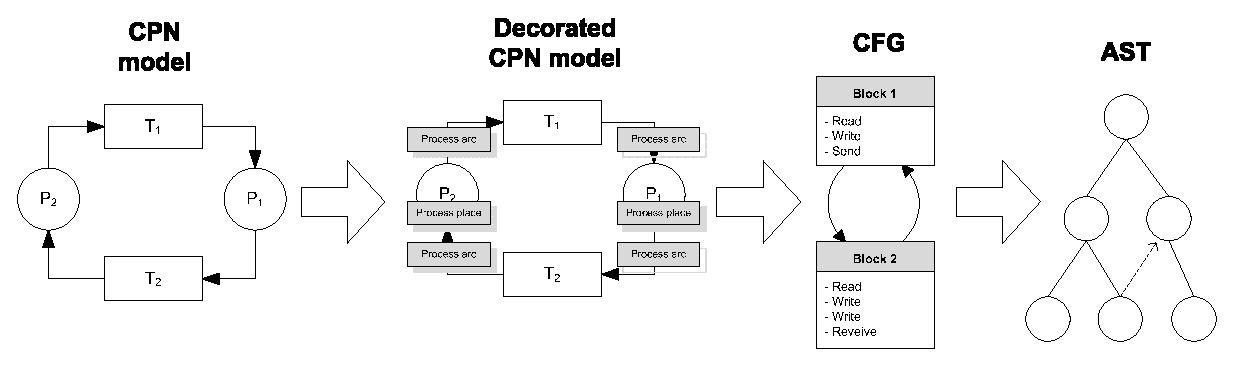
\includegraphics[width=\textwidth]{translation/graphics/phasesfigure01.eps}
\caption{The first three phases of the translation}
\label{fig:translationphases123}
\end{figure}

The first phase consists of decorating the different parts the CPN model with types. The CPN model is assumed to be a ProPCPN model as defined in section \ref{chap:netclass}. The second phase translates from the decorated CPN model into a control flow graph (CFG). A CFG representing the control flow is constructed for each process partition. In the third phase the CFG is translated into an abstract syntax tree (AST) for a simple language. We have designed the language to be abstract enough such that it can be translated into any common type of programming language. The control flow represented by the structure of the CFG is made explicit by, e.g., goto statements in the AST. 

\begin{figure}
\centering
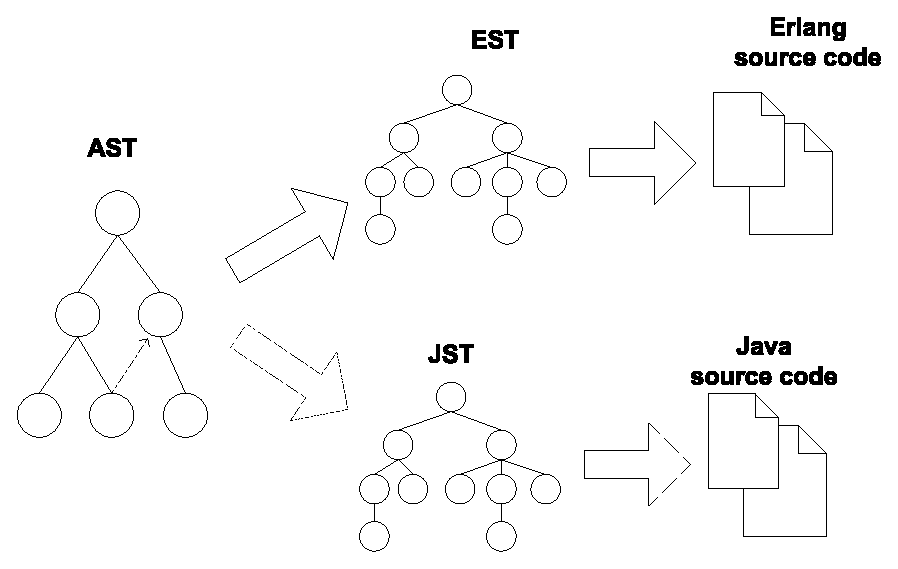
\includegraphics[scale=0.75]{translation/graphics/phasesfigure02.eps}
\caption{The last two phases of the translation}
\label{fig:translationphases45}
\end{figure}

The last two phases of the translation are illustrated in Fig.~\ref{fig:translationphases45}. These phases are language dependent, i.e., the phases are designed for a specific programming language. In Fig.~\ref{fig:translationphases45} two possible target language are illustrated. In the top of the figure, the AST is translated into an Erlang syntax tree (EST) and then into Erlang source code. In the bottom of the figure, the AST is translated into a Java syntax tree (JST) and then into Java source code. We have choosen Erlang as the target language, thus the AST is translated into an EST. The EST can then be transformed into a textual representation by traversing it and printing the nodes according to the Erlang grammar.

\section{Phase 1: Decorating the CPN Model}
\label{sec:cpntodcpn}
The purpose of this phase is to identify different parts of the CPN model and decorate them with a type. This is done in order to simplify the translation from the CPN model to the CFG. This phase uses properties of the ProPCPN net class to perform the identification.

\subsection{Finding Process Partitions}
This phase assumes that the CPN model is a ProPCPN model. When a ProPCPN model is decorated the first thing that needs to be done is to divide it into \emph{process partitions}, i.e., for every node and arc identify which process partition they belong to and decorate them with this information. This is done by using the information provided by the declarations in the ProPCPN model. A process partition is defined with an index colour set declaration which has \code{declare pid} attached to it. The producer-consumer model contains the following declaration:

\begin{verbatim}
colset PRODUCER = index p with 1..2 declare pid;
\end{verbatim}
 
This declaration is an index colour set declaration with a range from 1 to 2, and it has \code{declare} \code{pid} attached. The definition of ProPCPNs defines this to be a process partition named \code{PRODUCER}. The \emph{process variable} related to the process partition is a variable declaration with the type \code{PRODUCER}. In the producer-consumer model we find the declaration:

\begin{verbatim}
var prod : PRODUCER;
\end{verbatim}

This declaration is a variable declaration with the variable name \code{prod} of type \code{PRODUCER}. According to the definition this is a process variable of the \code{PRODUCER} process partition. Analogously, declared index colour set and variable can be found for the \code{CONSUMER} process partition.

\subsection{The Steps of the Decoration}
To illustrate how decorating works for the producer of the producer-consumer system we have decorated the model with labels specifying what type a place or an arc has. The decoration has six steps which are presented in turn.

\begin{description}
\item[Step 1] In this step all \emph{process places} are decorated with the process place type and the corresponding process partition. This is done using the assumption from the definition that only process places have the process type as colour set. Both the \code{PRODUCER} and the \code{CONSUMER} process partitions have two process places, e.g., the places \figitem{Producing} and \figitem{Sending} are labelled as process places for the \code{PRODUCER} process partition since they have the type \code{PRODUCER}. The decoration of the producer process partition can be seen in Fig.~\ref{fig:decoratedproducerconsumerprocessplaces}.

\begin{figure}[h!]
\centering
\includegraphics[width=\textwidth]{translation/cpn_to_dcpn/graphics/decorated_model_process_places.eps}
\caption{The producer decorated with process places}
\label{fig:decoratedproducerconsumerprocessplaces}
\end{figure}

\item[Step 2] The \emph{transitions} in the model are decorated with the process partition they belong. According to the definition, it is only allowed for transitions to move process tokens from its own process partition. Furthermore, a transition must move at least one process token, thus the process partition of the connected process places determine the process partition of the transition. The transitions \figitem{ProduceData} and \figitem{SendData} are both connected to process places from the \code{PRODUCER} process partition and therefore these transitions belong to this partition.

\item[Step 3] Then, \emph{local places} are identified. The definition specifies that for a place to be a local place it must only be connected to transitions from a single process partition. A local place also has the product colour set, where the first component is a process type, and the second component is a data. Since all transitions already have been decorated with their process partition, the task is to look at places with the above mentioned colour set and check that the transitions connected to that place all belong to the same process partition. The producer-consumer model has three local places, namely \figitem{Data}, \figitem{ProducedData} and \figitem{ReceivedData}. These are local places because they have a colour set of the correct form, and they are only connected to transitions from one process partition. The decoration of the producer process partition with local places, buffer places, and shared places can be seen in Fig.~\ref{fig:decoratedproducerconsumerotherplaces}.

\begin{figure}[h!]
\centering
\includegraphics[width=\textwidth]{translation/cpn_to_dcpn/graphics/decorated_model_other_places.eps}
\caption{Decoration with local places, a buffer place, and a shared place}
\label{fig:decoratedproducerconsumerotherplaces}
\end{figure}

\newpage

\item[Step 4] Next, the \emph{buffer places} are decorated. They have colour sets on the same form as local places, but they are connected to transitions from more than one process partition. The place \figitem{Buffer} is the only buffer place in the model.

\item[Step 5] The last places to be identified are \emph{shared places}. They are the only places which have a non-process colour set, and that are not a pair with a process identifier. The place \figitem{NextConsumer} is identified as a shared place because the colour set of this place is not a product and not a process type.

\item[Step 6] In the final step of the decoration the \emph{arcs} are decorated. Arcs are decorated according to the type of place they are connected to, e.g., the arcs connected to the local place \figitem{Data} are local arcs. Similar the arc from \figitem{ProduceData} to \figitem{Sending} is a process arc. The decoration of the producer process partition with arc types can be seen in Fig.~\ref{fig:decoratedproducerconsumerallarcs}.
\end{description}

\begin{figure}[h!]
\centering
\includegraphics[width=\textwidth]{translation/cpn_to_dcpn/graphics/decorated_model_all_arcs.eps}
\caption{The producer-consumer CPN model decorated arc types}
\label{fig:decoratedproducerconsumerallarcs}
\end{figure}

After these steps, all nodes and arcs in the CPN model have been decorated. The model is now ready to be translated from a CP-net into a control flow graph.

\section{Phase 2: Translating the Decorated CPN Model to a CFG}
\label{sec:dcpntocfg}
The main purpose of this phase is to extract the control flow from the decorated CPN model and make it explicit in a control flow graph (CFG). This phase also identifies common program constructs, e.g., processes, variable, and access to variables. Furthermore, the phase finds synchronisation points, i.e., messages passing between processes. The CFG we use is a directed graph in which arcs correspond to control flow and nodes corresponds to a sequence of statements to be executed.

\subsection{Performing the Translation}
\label{sec:cpntranslation}
Given the decorated CPN model belonging to the class ProPCPN, this phase translates it into a CFG. With the decorated CPN model it is straightforward to operate on a model from a process partition perspective, e.g., to iterate through all process places in a given process partition. A CFG is constructed for all process partition in the model, thus in the producer-consumer system two CFGs are generated: one for the \code{producer} process partition and one for the \code{consumer} process partition. In Fig.~\ref{fig:prodconscfg} we see the translated CFG for the \code{producer} process partition. Below we explain how it is obtained from the decorated ProPCPN model.

\begin{figure}[b!]
\centering
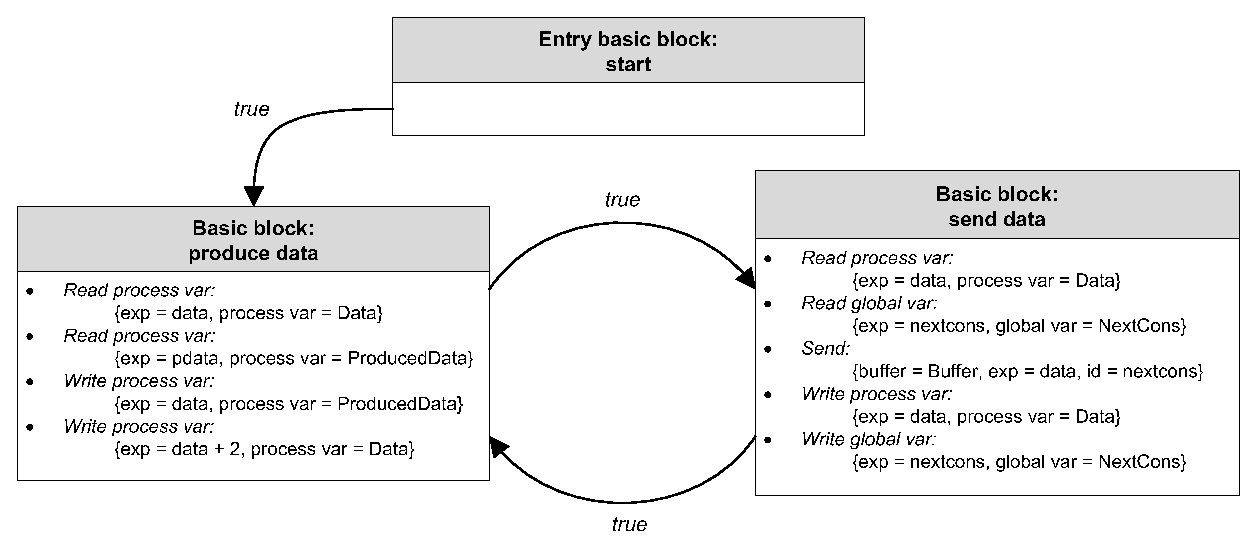
\includegraphics[width=\textwidth]{translation/dcpn_to_cfg/graphics/producerconsumercfg.eps}
\caption{The CFG of the producer process}
\label{fig:prodconscfg}
\end{figure}

%The initial state of each process instance is extracted form the initial marking of the process partition. This information is carried along in the variables for each process partition in the CFG.  \fxnote{maybe move this to another place?}

\subsubsection{Local Places}
In the CPN model, process instances use local places to store data. In a programming language this corresponds to reading/writing a variable, thus a local place is translated into a CFG \emph{process variable}. The name process variable indicates that the scope of these kinds of variables is within a given process. The \code{producer} process partition contains the two process variables \code{Data} and \code{ProducedData} corresponding to the two local places \figitem{ProducedData} and \figitem{Data} in the CPN model. 

Since a local place has an initial marking it is important to carry along this information in the corresponding process variable. The initial expressions for the variables are extracted from the initial markings of the local places. In the producer-consumer system the initial marking of the local place \figitem{ProducedData} is empty, thus the initial expression of the corresponding process variable contains the empty expression. The CFG variable node \code{Data} contains two initial expressions for the two \code{producer} process instances. In general, a process variable contains an initial expression for each process instance. 


\subsubsection{Buffer Places}
In a ProPCPN model, process instances use buffer places to share data with a particular process instance. In a programming language this corresponds to sending to and receiving from a buffer, thus a buffer place is translated into a \emph{buffer} in the CFG. In the producer-consumer system there is one buffer corresponding to the buffer place \figitem{Buffer}.


\subsubsection{Shared Places}
Process instances use shared places in the CPN model to share data with multiple process instances. In a programming language this corresponds to a global variable or some shared memory where process instances can share data. Shared places are therefore translated into \emph{global} variables in the CFG. In the producer-consumer system there is one global variable corresponding to the shared place \figitem{NextConsumer}. The initial marking of the shared place is extracted and carried along in the global variable. 

\subsubsection{Transitions}
Transitions in the CPN model are translated into \emph{basic blocks} in the CFG. In the producer process partition (see Fig. \ref{fig:prodconscfg}) the transition \figitem{ProduceData} is translated into the basic block \code{produce data} and the transition \figitem{SendData} is translated in the basic block \code{send data}. An item in a basic block in Fig.~\ref{fig:prodconscfg} should be read as follows: the name of the statement is written in italic, and the body of the statement is written in curly brackets. 

The basic block is constructed from the input and output arcs to and from the transition. Arcs are translated depending on the type of the arc. In the decorated CPN model, the connected arcs are labelled with types. In the following we consider arcs connecting transitions to local places, shared places, and buffer places.

\paragraph*{Arcs connecting a transition to a local place.}
An input arc with a arc expression on the form \code{(pid, var)} from a local place to a transition corresponds to process instance \code{pid} reading a variable \code{var}. Consider the input arc expression \code{(prod, data)} from the local place \figitem{Data} to the transition \figitem{ProduceData}. This arc is translated to a \emph{Read process var} with the expression \code{data} as shown in Fig.~\ref{fig:prodconscfg}. The \emph{Read process var} also has a pointer to the process variable \code{Data} since this is where it gets its input from.

An output arc expression on the form \code{(pid, exp)} from a transition going to a local place corresponds to process instance \code{pid} writing an \code{exp} to a variable \code{var}. Consider the output arc expression on the arc from the transition \figitem{ProduceData} to the local place \figitem{ProducedData}. This is translated to a \emph{Write process var} (seen in Fig.~\ref{fig:prodconscfg}) containing the expression \code{data} which is extracted from the CPN model. The \emph{Write process var} has a pointer to the variable \code{ProducedData} since this is where the value should be written to.

\paragraph*{Arcs connecting a transition to a buffer place.}
An input arc with the arc expression \code{(pid, var)} from a buffer place to a transition corresponds to a process receiving a message which is put into a variable \code{var}. This kind of input arc can be found in the consumer part of the producer-consumer system on the input arc (with the expression \code{(cons, data)}) from the buffer place \figitem{Buffer} to the transition \figitem{ReceiveData}. This is translated into a \emph{receive} which has the expression \code{data} meaning that the value of the received data should be read into the variable \code{data} for later use. 

An output arc with the arc expression on the form \code{(pid, exp)} from a transition to a buffer place corresponds to sending an expression \code{exp} to a process instance \code{pid}. Consider the output arc expression \code{(nextcons, data)} from the transition \figitem{SendData} to the buffer place \figitem{Buffer}. As seen in Fig.~\ref{fig:prodconscfg} this is translated a \emph{send} which points to the CFG \emph{buffer}. It contains the expression \code{data} and the receiver process instance \code{nextcons}.

\paragraph*{Arcs connecting a transition to a shared place.}
An input arc with the arc expression \code{var} from a shared place to a transition corresponds to a process reading a variable with a global scope, i.e., a variable that can be accessed and modified by multiple process instances. 

In the producer-consumer system there is a input arc expression \code{nextcons} to the transition \figitem{SendData} from the shared place \figitem{NextConsumer}. As seen in Fig.~\ref{fig:prodconscfg} this is translated to a \emph{Read global var} which points to the global variable \code{NextConsumer} and contains the expression \code{nextcons}. 

An output arc with the arc expression \code{var} from a transition to a shared place corresponds to a process writing to a global variable. Consider the output arc expression to the transition \figitem{SendData} from the shared place \figitem{NextConsumer}. This is translated to a \emph{Write global var} which points to the global variable \code{NextConsumer} and contains the expression \code{nextcons}.

\subsubsection{Process Places}
Process places in the CPN model are not explicitly translated into nodes in the CFG, but instead represented as edges between basic blocks. The idea is, for each basic block, to have a set of reachable basic blocks. In Fig.~\ref{fig:prodconscfg} we see that the basic block \code{produce data} has an edge to \code{send data} which means that after executing \code{produce data} the control should flow to the basic block \code{send data}. The condition \code{true} on the edge indicates that it is an unconditional flow of control. There is a special \emph{entry} basic block for each CFG that represent the starting point of the program. In Fig.~\ref{fig:prodconscfg} it points to the basic block \code{produce data}. In section \ref{sec:advancedissues} we explain how conditional flows are handled.

\subsection{The Structure of the Control Flow Graph}
\label{sec:cfgebnf}
A CFG is created for each process in the program, e.g., one CFG for the \code{producer} process and one for the \code{consumer} process. The CFG is a directed graph where the nodes in the graph are connected by labelled edges. The nodes in the graph represent the basic blocks and the edges represent the control flow between the blocks. The labels on the edges are \emph{conditions}, i.e., a list of boolean expressions, specifying whether the control flow can follow this edge or not.

The CFG contains a special entry basic block which is always the starting point for the control flow. The entry basic block only has outgoing edges because the control is never supposed to return to the entry point. 

The basic blocks in the CFG contains a collection of statements, e.g., read, write, send, and receive statements. Taking a closer look at, e.g. read statements, we can see that they contain a pointer to a process variable and an expression. The expression specifies a local variable that the value of the process variable is to be read into.

\section{Phase 3: Translating the CFG to an AST}
\label{sec:cfgtoast}
The main purpose of this phase is to take the control flow given in the structure of the control flow graph (CFG) and translate it into a tree form consisting of nodes representing common programming constructs, e.g., jump statements. Furthermore, read and write expressions contained in the CFG are parsed and translated into subtrees in order to make the there structure explicit in the produced tree.

\subsection{Performing the Translation}
The tree this phase produces is an abstract syntax tree (AST) for a simple language that contains common program constructs, e.g., jump statements, read and write statements and conditional statements. The AST contains a node for each program construct. The root node is a \emph{program node} that contains a number of \emph{processes} and \emph{global variables}. A process has a number of \emph{blocks}. This is the basic structure of the AST and to explain the translation we look at how the CFG for the producer-consumer system is translated into an AST. Fig.~\ref{fig:producerast} shows a subtree of the AST where only the nodes from the \code{produce data} block of the \code{producer} process is shown.

\begin{figure}
\centering
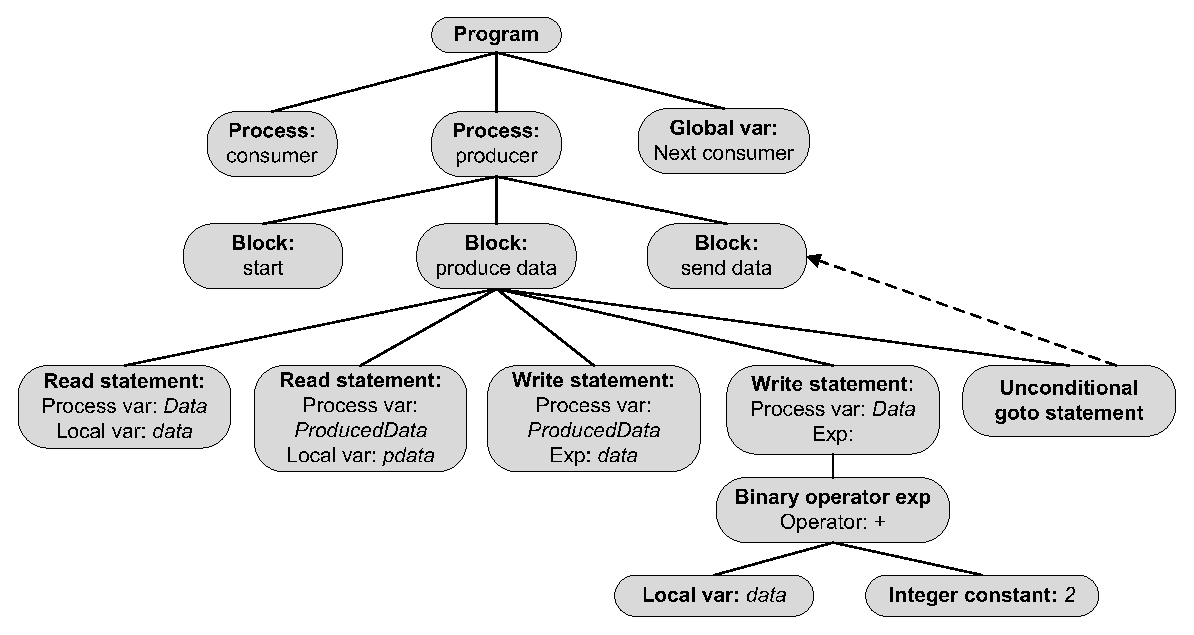
\includegraphics[width=\textwidth]{translation/cfg_to_ast/graphics/producerast.eps}
\caption{The AST for the "produce data" part of the producer}
\label{fig:producerast}
\end{figure}

When building the AST a process is created for each CFG process. As Fig.~\ref{fig:producerast} shows the program contains two processes, namely the \code{producer} and the \code{consumer}. The program node also contains the global variable \code{NextConsumer}. In the CFG each process contains a number of variables. These variables are translated into process variables local to each process. A process variable contains an initial expression for each instance of the process. Each initial expression is parsed and if not recognised an unknown expression is inserted. An AST process also has a number of AST blocks which are created from the basic blocks of the CFG. The \code{producer} process contains three blocks: \code{produce data}, \code{send data}, and \code{start}. Below, we explain how the block \code{produce data} is created.

\paragraph*{Read statements.} The first two child nodes in the \code{produce data} block are \emph{read statements}. These are translated from the two readings in the CFG of the process variables \code{Data} and \code{ProduceData}, respectively. A read statement contains both a \emph{local variable} and a \emph{process variable}. A local variable is a variable that is local to the block, and a process variable is local to the process. The value of a process variable is read into a local variable, e.g., the first read statement reads the value of the process variable \code{Data} into the local variable \code{data}.

\paragraph*{Write statements.} The next two nodes of the block are \emph{write statements} which write values to process variables. These are translated from the two writings in CFG to the process variables \code{ProduceData} and \code{Data}, respectively. Write statements contain an expression which becomes the new value of the process variable. The expression can, e.g., be the value of a local variable or an arithmetic expression.

The first write statement writes the value of the local variable \code{data} to the process variable \code{ProducedData}. The second write statement writes a value the process variable \code{Data}. This value is a binary operator expression which on the left hand side has the value of the local variable \code{data} and on the right hand side the integer constant \code{2}. This expression shows an example of how the structure of expressions are represented in the AST.

\paragraph*{Goto statements.} The rightmost node in the \code{produce data} block is an \emph{unconditional goto statement} which is a jump statement without a condition. It has a pointer to the block it jumps to which in this case is the \code{send data} block. The jump statements are translated from edges between basic blocks in the CFG. An AST has two types of goto statements, namely a unconditional without a condition, and a conditional which has a condition attached to it. The condition is a boolean expression specifying whether the jump should be made or not. Common for both types is that they have a pointer to an AST block which is the target of the goto statement.

\begin{figure}[b!]
\centering
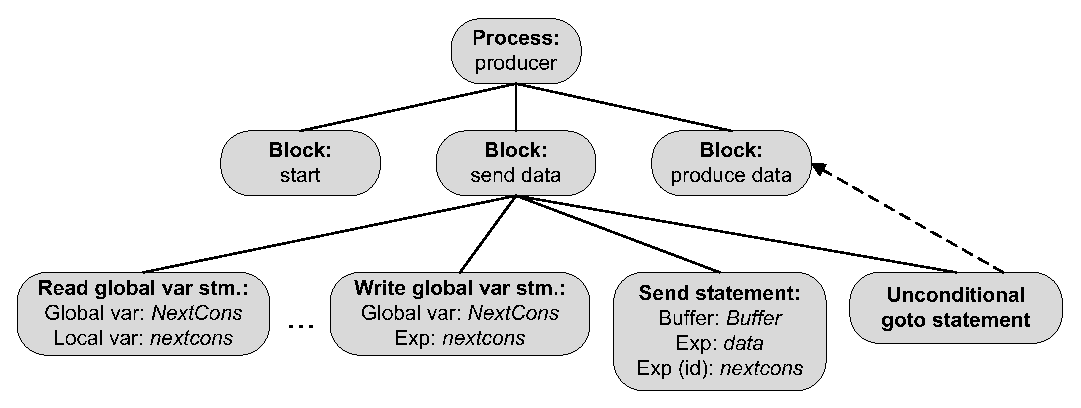
\includegraphics[scale=0.7]{translation/cfg_to_ast/graphics/producersendast.eps}
\caption{The AST for the "send data" part of the producer}
\label{fig:producersendast}
\end{figure}

\paragraph*{Read and write to and from global variables.}
Fig.~\ref{fig:producersendast} shows the "send data" part of the \code{producer} process. The three dots between the two first nodes indicates that we have left out a read and a write statement which reads the value of the process variable \code{ProducedData} into the local variable \code{data} and writes the same value back to \code{ProducedData} leaving it unchanged.

The first node in the \code{send data} block is a \emph{global variable read statement} which reads the value of the global variable \code{NextCons} into the local variable \code{nextcons}. This is very similar to a read statement from a process variable. The read statements of global variables are translated from the readings of global variables in the CFG.

The \emph{global variable write statements} are translated from writings of global variables from the CFG and are also very similar to writings to process variables. The second node in Fig.~\ref{fig:producersendast} writes the value of the local variable \code{data} to the global variable \code{NextCons}.

\paragraph*{Send statements.} The third node in the \code{send data} block is a \emph{send statement}. A send statement contains a pointer to the buffer that is to receive the message, and an expression that specifies the process identifier of the receiving process. With this information, a process is able to send a message to a specific buffer for a specific process. A send statement also contains an expression which specifies the value which is sent.

Send statements are translated from the send statements in the CFG. In Fig.~\ref{fig:producersendast} the send statement is to send the value of the local variable \code{data}, which was read from the process variable \code{ProducedData}. This value should be send to the buffer \code{Buffer} for the process which is identified by the value of \code{nextcons}, that was read from global variable \code{NextCons}.

\paragraph*{Receive statements.} Messages are received using a \emph{receive statement}. A receive statement has a pointer to a buffer where the incoming messages are stored and where the process can read the messages from. It also contains a local variable into which a message from the buffer is read. The receive statements are translated from the receive statements in the CFG. An example of the use of a receive statement is found in the \code{consumer} process when it receives the produced data from a \code{producer} process.

\subsection{The Structure of the AST}
% Forklar EBNF

\begin{figure}[b!]
\footnotesize
\begin{verbatim}
<Program>                    ::= *<Process> *<GlobalVariableDeclaration>
<GlobalVariableDeclaration>  ::= <Name> <InitialExpression>
<Process>                    ::= <Name> *<Block> <EntryBlock> 
                                        *<ProcessVariableDeclaration>
<Name>                       ::= string
<ProcessVariableDeclaration> ::= <Name> <InitialExpression>
<InitialExpression>          ::= <Expression>
<Block>                      ::= <Name> <Statements>
<EntryBlock>                 ::= <Block>
<Statements>                 ::= *<Statement> |
                                 <Statements> <UnconditionalGotoStatement>
<Statement>                  ::= <LocalVariableDeclaration> |
                                 <ReadStatement> | <ReceiveStatement> |
                                 <GlobalVariableReadStatement> |
                                 <WriteStatement> | <SendStatement> |
                                 <GlobalVariableWriteStatement> |
                                 <ConditionalGotoStatement>
...
<Expression>                 ::= <BinaryOperatorExpression> |
                                 <LocalVariableExpression> |
                                 <GlobalVariableExpression> |
                                 <ProcessVariableExpression> |
                                 <UnknownExpression> |
                                 <IntegerConstantExpression> |
                                 <StringExpression> | <Undefined>
...
\end{verbatim}
\normalsize
\caption{The EBNF for the abstract syntax tree}
\label{fig:ASTEBNF}
\end{figure}


In order to explain the structure of the AST more precisely we describe it using the Extended Backus-Naur Form (EBNF) \cite{EBNF}. Part of it is shown in Fig.~\ref{fig:ASTEBNF} and the full version can be found in appendix \ref{app:astebnffull}. The first definition is a \code{Program} which consists of zero or more processes and zero or more global variable declarations. A \code{GlobalVariableDeclaration} is a declaration of a variable that can be accessed by every running process in the program, i.e., a variable which is shared between processes. The \code{GlobalVariableDeclaration} consists of a name, which is a string, and an initial expression which is used to initialise the global variable.

A \code{Process} has a name which is simply a string. It has zero or more \code{Block}s which is a named block of statements. Furthermore, a \code{Process} has one or more \code{ProcessVariableDeclaration}s which is declarations of variables that can be accessed anywhere within the process. Finally, a \code{Process} has a \code{StartBlock} which is the first block of statements to be executed in the process.

Taking a closer look at the \code{Statement} and \code{Statements} constructions we see that they contain both a \code{ConditionalGotoStatement} and an \code{Unconditional}-\code{GotoStatement} which represents goto statements with or without an attached condition, respectively. The construction is made in such a way that if an \code{UnconditionalGotoStatement} appears there cannot appear other types of statements afterward. This is done to avoid unreachable statements.

The last construction in the EBNF is \code{Expression} which consists of all the types of expressions in the AST. We have chosen only to support a small set of expressions. E.g., we have chosen \emph{Binary Operator Expressions} to illustrate how expressions can be parsed from CPN ML into a tree structure fitting the AST. Other expressions are simply wrapped in an \code{UnknownExpression} which contains the expression as the original string. The type \code{Undefined} is used when, e.g., a variable has no initial value.

\section{Phase 4: Translating the AST to an EST}
\label{sec:astest}

This phase generates an Erlang syntax tree (EST) based on an AST. The purpose of this phase is to translate the abstract representation of a program into an Erlang program represented as a tree. The control flow, represented by goto statements in the AST, is translated into the functional language paradigm equivalent \emph{function calls}. Since functional languages are stateless the state is passed along in the function calls. Processes are native in the Erlang language, thus each process in the AST is simply translated into a module. The generated modules are spawned in a special \emph{system} module.

\begin{figure}[b!]
\centering
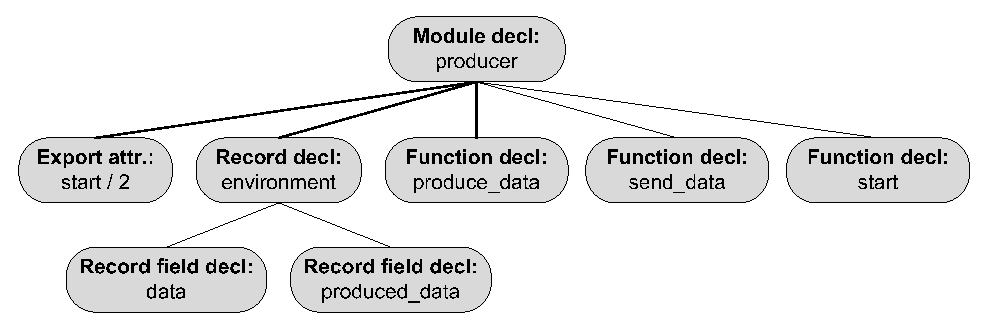
\includegraphics[width=\textwidth]{translation/ast_to_est/graphics/producerest01.eps}
\caption{The producer module of the EST}
\label{fig:prodmoduledecl}
\end{figure}

To give an impression of the translation from an AST to an EST we take a look at the producer-consumer system. Figure \ref{fig:prodmoduledecl} shows how a part of the producer is represented in the generated EST. In the following we explain how this EST and some of its subtrees are created.

\subsection{Performing the Translation}
In this section we first describe how AST processes are translated into EST module declarations. Next, we describe how global variables are translated into modules which can be used to share data among processes. Then we explain how AST blocks are translated into functions, and how a \code{start} function is created in each module. At the end of this section we describe a special system module responsible for spawning process instances.

\subsubsection{Process Nodes in the AST}
For each AST process node we create an EST \emph{module declaration}. Figure \ref{fig:prodmoduledecl} shows the \code{producer} module declaration for the producer-consumer system. AST processes contain process variables which are shared among blocks in that specific process. This kind of variables are not directly supported in Erlang, but by having a dedicated \emph{environment} record which is carried along in the function calls we get the same result as with process variables. For each AST process variable a field with the same name is created in the environment record. In Fig. \ref{fig:prodmoduledecl} we see the record declaration \code{environment}. There are two process variables \code{produced\_data} and \code{data} in the AST, thus the environment contains two \emph{record field declarations} corresponding to \code{produced\_data} and \code{data}.

\subsubsection{Global Variable Declarations}
Global variables in the AST are used to share data between processes. There is no native equivalent to global variables in the Erlang language, but instead we have constructed a module which can be used to spawn processes that acts like global variables. The module we create is identical to the module \code{shared} described in section \ref{subsec:thesharedstore}.

\subsubsection{Block Nodes in the AST}
An AST process contains a number of blocks describing the behaviour of the process. Blocks are translated into \emph{function declarations} in the EST. The \code{producer} module declaration thus contains two function declarations: \code{produce\_} \code{data} and \code{send\_data} as seen in Fig.~\ref{fig:prodmoduledecl}. Fig.~\ref{fig:prodproducefunc} shows the function declaration corresponding to the AST block \code{produce data}. As mentioned earlier the environment is given as argument to each function, thus an EST \emph{variable} \code{Env} is added to the argument list of the function declaration. 

\begin{figure}
\centering
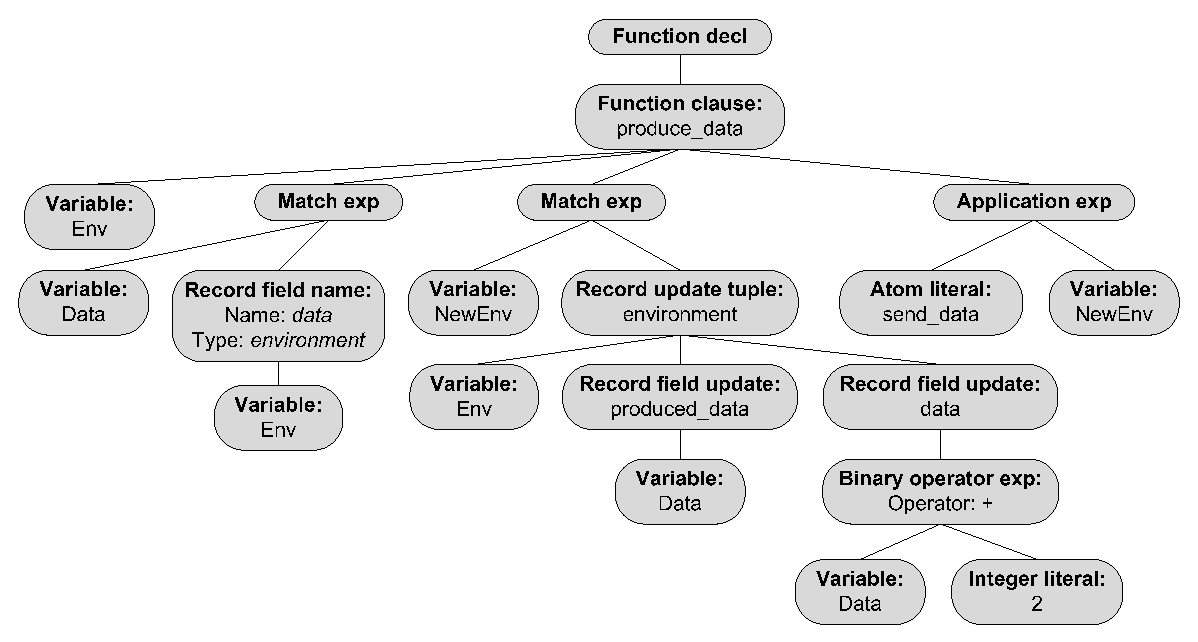
\includegraphics[width=\textwidth]{translation/ast_to_est/graphics/producerest02.eps}
\caption{The function declaration \code{produce\_data}}
\label{fig:prodproducefunc}
\end{figure}

Notice that since the EST is used by phase 5 to print the tree in a depth first traversal, the order of the EST nodes determine the semantic of the resulting Erlang program. Because, e.g., a read variable can be used to update another variable, it is important to do the reading of process variables, reading of global variables and receiving data from buffers, before writing to process variables, writing to global variables or sending data to buffers.

\paragraph*{Read process variable statements.} 
Reading a process variable is done in Erlang by accessing the corresponding field in the environment. In the EST this becomes a lookup in the record for the field with the same name as the process variable. This value is then bound to a variable which has the name given in the local variable expression of the read statement. This can be seen in Fig. \ref{fig:prodproducefunc} where the \emph{record field name expression} with the type \code{environment}, name \code{data}, and the variable \code{Env} is bound to the variable \code{Data}.

\paragraph*{Write process variable statements.}
In Erlang write statements for process variables corresponds to updating the field in the environment for that particular process variable. Fig. \ref{fig:prodproducefunc} shows how this update is represented in the EST. A \emph{record update tuple expression} containing the variable \code{Env} is bound to a variable \code{NewEnv}. The two \emph{record field update}s ensures that the fields \code{data} and \code{produced\_data} are updated corresponding to the write statements to the process variables.

\paragraph*{Receive statements.}
Receiving messages is a native construct in the Erlang language. The received messages are stored in a built-in Erlang buffer. To handle the translation of more advanced control flow constructs (presented in section~\ref{sec:advancedissues}) a buffer with extra functionality is needed. For this reason an explicit \code{buffer} process is used to receive messages. The Erlang code for the \code{buffer} module is found in appendix~\ref{appsec:buffer}. A dedicated buffer process is spawned for each receiving point of each process instance to make it equivalent to using the built-in Erlang buffers. The way to retrieve a message from the buffer is to send the atom \code{get} to the buffer process and the buffer process will send the first message in the buffer back to the requesting process.

Because of the \code{buffer} process, receiving messages it translated into sending a \code{get} request followed by a \emph{receive expression}. In the consumer module we find such an EST (see Fig.~\ref{fig:receiveexp}) in the function clause \code{receive\_data}. It consist of a send expression containing the name of the buffer and the atom literal \code{get}. This is followed by a receive expression with one \emph{receive clause} with the pattern consisting of a variable \code{Data}. The clause body contains one expression, namely the variable \code{Data}. This makes the variable (containing the received data) the return value of the receive expression and thus available in the remaining part of the function.

\begin{figure}[h!]
\centering
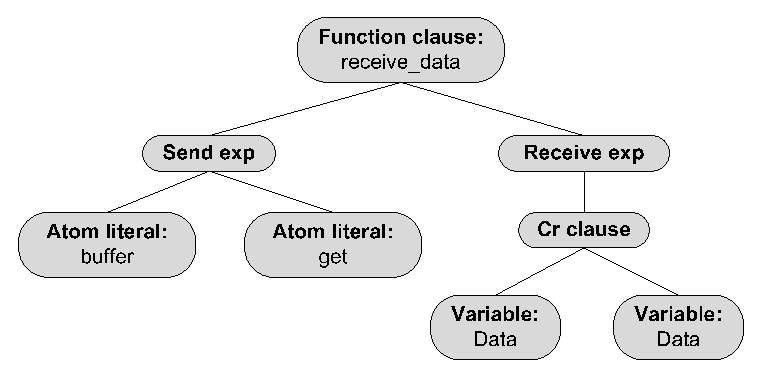
\includegraphics[scale=0.7]{translation/ast_to_est/graphics/producerest03.eps}
\caption{The receive expression subtree of the EST}
\label{fig:receiveexp}
\end{figure}

\paragraph*{Send statements.}
Since message passing is native in the Erlang language this is simply translated into a send expression in the EST. The recipient of the message is given by a buffer and an expression identifying the receiving process. In a send expression the identifier expression evaluates to an integer and together with the buffer it is possible to address the receiver of the message. The send expression furthermore contains an atom literal \code{send} indicating that the message should be added to the buffer. 

\paragraph*{Read global variable statements.}
As explained in section \ref{sec:producerconsumererlang} we have translated global variables into a shared process used to exchange data. Thus reading a global variable is translated to first sending a \code{\{get, id\}} request to the shared process corresponding to the global variable and then receiving some data from the shared process. In Fig. \ref{fig:readglobalvarexp} we see how this works in the \code{send\_data} function of the \code{producer} module. In the EST there is a \emph{send expression} containing the receiver \code{next\_consumer} and a \emph{tuple} containing the atom literal \code{get} and the application expression \code{self()}. An \emph{application expression} is a function call and the Erlang built-in function \code{self()} returns the process ID of the calling process. The send expression is then followed by a receive expression ready to receive the data from the shared process.

\begin{figure}[h!]
\centering
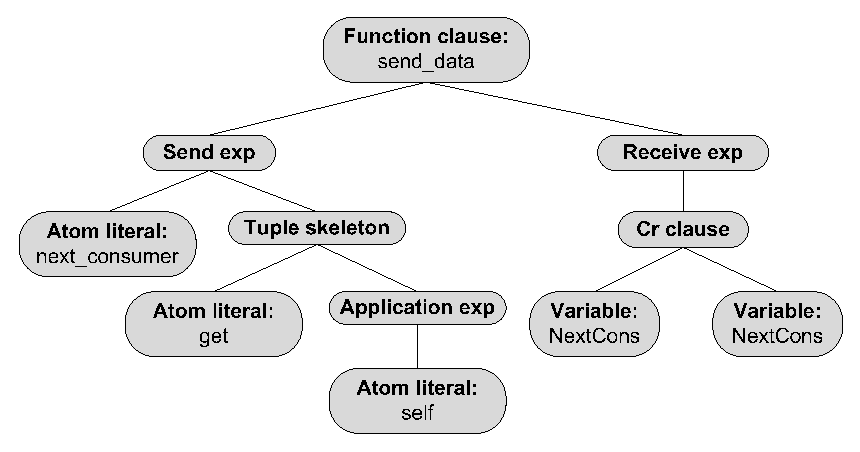
\includegraphics[scale=0.7]{translation/ast_to_est/graphics/producerest04.eps}
\caption{The subtree of the EST reading a global variable}
\label{fig:readglobalvarexp}
\end{figure}

\paragraph*{Write global variable statements.}
In the EST, write statements to global variables are translated into \emph{send expressions} which sends the value to be written to the shared process. The function \code{send\_data} contains a send expression which is a translation of the write statement to the global variable \code{NextConsumer}. This is done by sending a \emph{tuple} containing the atom literal \code{set} and the expression \code{nextcons}.

\paragraph*{Goto statements.}
\emph{Goto} statements in the AST are divided into \emph{unconditional} and \emph{conditional}. Unconditional goto statements are simply translated into application expressions in the EST. In the EST for the function \code{produce\_data} (see Fig.~\ref{fig:prodproducefunc}) we see the application expression containing the atom literal \code{send\_data} and the argument \code{NewEnv}. Conditional goto statements are explained in section \ref{sec:advancedissues}. 


\subsubsection{The Start Function}
The purpose of the \code{start} function is to initialise the environment in the process and call the first function to be executed. The start function takes a number of arguments used to initialise the environment. For each AST process variable an EST variable with the same name as the process variable is added to the function clause argument list. This can be seen in Fig.~\ref{fig:startfunction} showing the \code{start} function in the module \code{producer}. The function clause contains a variable \code{Produced\_data} and a variable \code{Data} as arguments corresponding to the process variable of the same names.  

\begin{figure}[h]
\centering
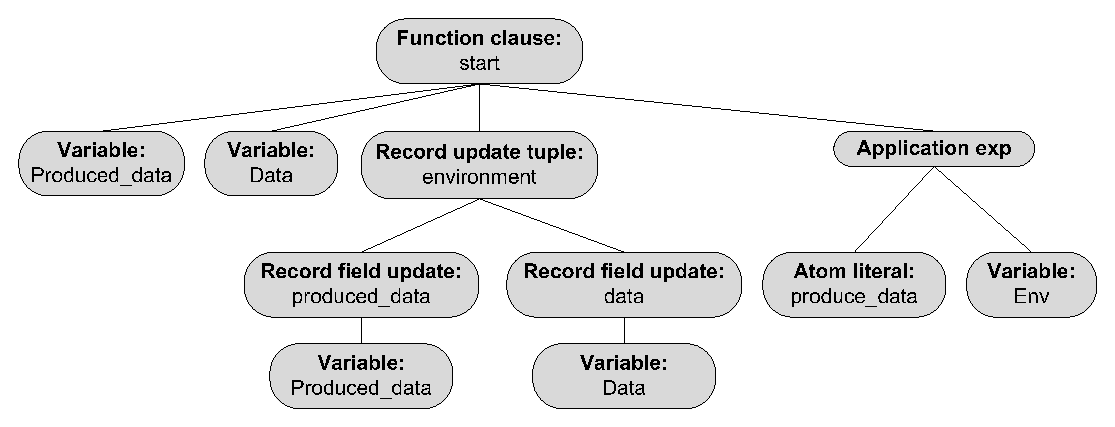
\includegraphics[width=\textwidth]{translation/ast_to_est/graphics/producerest05.eps}
\caption{The subtree of the EST showing the \code{start} function clause}
\label{fig:startfunction}
\end{figure}

The environment is then initialised by creating an environment record where the arguments are used to update to corresponding field. This record is then bound to the variable \code{Env}. In Fig.~\ref{fig:startfunction} this is seen in the match expression where a record update tuple expression is matched to the variable \code{Env}. The record update tuple expression contains two record field update expression: one assigning the variable \code{Produced\_data} to the field \code{produced\_data}, and one assigning the variable \code{Data} to the field \code{data}.

In an AST process there is a entry block which contains a goto statement to the first block to be called. In the EST, an application expression is created calling the function corresponding to the first block. In the \code{producer} module the start function shown in Fig.~\ref{fig:startfunction} calls the function \code{produced\_data}.

The \code{start} function is exported in the module such that it can be called from outside. This can be seen in Fig. \ref{fig:prodmoduledecl} where an \emph{export attribute} exports the \code{start} function taking two arguments.

\subsubsection{Spawning the Process Instances}
We have chosen to have a dedicated module which spawns a process for each process instance. It also spawns the \code{buffer} processes and a \code{shared} process for each global variable. In Fig.~\ref{fig:systemmoduledecl}, the \code{start} function clause of the \code{system} module for the producer-consumer system is shown. It is responsible for spawning process instances, thus in the producer-consumer system this becomes: two producers, two consumers and two buffers belonging to those consumers, and a shared instance. In the \code{start} function clause we find an application expression calling the Erlang built-in function \emph{register} given a name and an application expression calling the Erlang built-in function \emph{spawn}.

\begin{figure}[h]
\centering
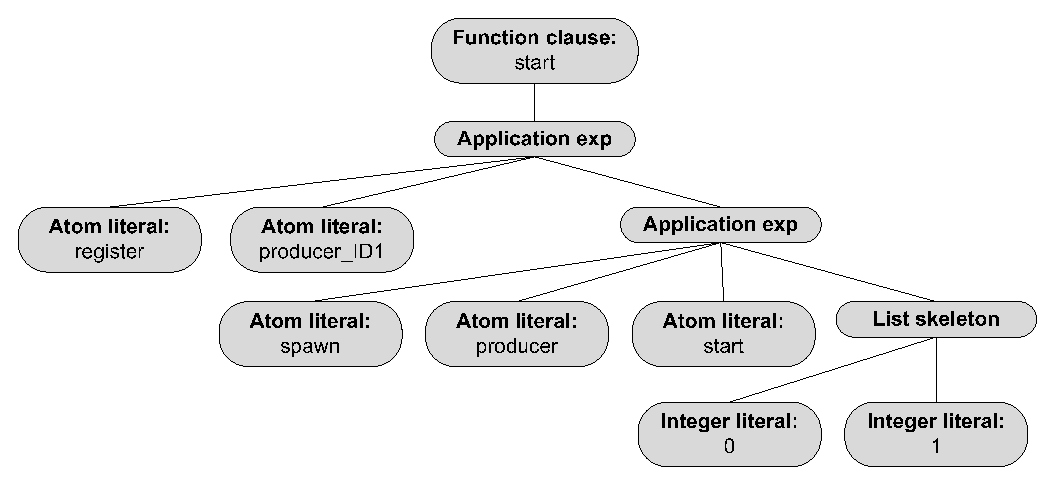
\includegraphics[width=\textwidth]{translation/ast_to_est/graphics/producerest06.eps}
\caption{The function clause \code{start} of the \code{system} module}
\label{fig:systemmoduledecl}
\end{figure}

\subsection{The Structure of the EST}
We describe the EST using EBNF and part of it is shown in Fig.~\ref{fig:ESTEBNF} (the full version can be found in appendix \ref{app:estebnffull}). The EST EBNF is based on the Erlang language specification grammar \cite{RefWorks:91}. The first definition is a \code{Program} which consists of zero or more \code{ModuleDecl}s. A \code{ModuleDecl} has a name, zero or more \code{HeaderForm}s and a \code{ProgramForm}. A \code{HeaderForm} is used to export functions and declare records. A \code{FunctionDecl} consist of a number of \code{FunctionClause}s which contains a function symbol, zero or one \code{pattern} (the arguments to the function clause) and zero or more \code{expression}s (the body of the function clause). A \code{Pattern} is, e.g., an atom literal, or a variable. An \code{Expression} is can be a \code{ApplicationExp}, \code{AtomicLiteral}, \code{BinaryOperatorExp}, \code{MatchExp}, \code{ReceiveExp}, \code{RecordExp}, \code{SendExp}, or a \code{Variable}. An \code{ApplicationExp} contains an expression (which could be an \code{AtomLiteral}) specifying which function to call, and a list of expressions which is the arguments to the function call.
\begin{figure}
\footnotesize
\begin{verbatim}
<Program>              ::= *<ModuleDecl>
<ModuleDecl>           ::= <ModuleName> *<HeaderForm> <ProgramForm> 
<ModuleName>           ::= string
<HeaderForm>           ::= <ExportAttribute> | <RecordDecl>
<ProgramForm>          ::= <FunctionDecl> | 
                           *<ProgramForm> <FunctionDecl> |
                           *<ProgramForm> <RecordDecl> 
<ExportAttribute>      ::= *<FunctionName>
<FunctionDecl>         ::= *<FunctionClause>  
<FunctionName>         ::= <FunctionSymbol> <arity>
<FunctionClause>       ::= <FunctionSymbol> ?<Pattern> *<Expression>
<Pattern>              ::= <AtomicLiteral> | <Variable>
... 
<AtomicLiteral>        ::= string
<Variable>             ::= string
<Expression>           ::= <ApplicationExp> | <AtomicLiteral> |
                           <BinaryOperatorExp> | <MatchExp> | <ReceiveExp> |
                           <RecordExp> | <SendExp> | <Variable> 
...
<ApplicationExp>       ::= <Expression> *<Expression>
<BinaryOperatorExp>    ::= <Expression> <Operator> <Expression>
<MatchExp>             ::= <Pattern> <Expression>
<ReceiveExp>           ::= *<CrClause>
<CrClause>             ::= <Pattern> *<Expression>
<RecordExp>            ::= ?<Expression> <RecordType> <RecordFieldNameExp> |
                           ?<Expression> <RecordType> <RecordUpdateTupleExp>
<RecordFieldNameExp>   ::= <RecordFieldName> 
<RecordUpdateTupleExp> ::= *<RecordFieldUpdate>
<RecordFieldUpdate>    ::= <RecordFieldName> <Expression>
<SendExp>              ::= <Expression> <Expression>
\end{verbatim}
\normalsize
\caption{The EBNF for the Erlang syntax tree}
\label{fig:ESTEBNF}
\end{figure}

\section{Phase 5: Translating the EST to Erlang Code}
\label{sec:esttocode}

The last phase is translating the Erlang syntax tree (EST) into a textual representation. The EST is a concrete representation of Erlang so the task is to traverse the tree, and print a textual representation of each node to a file. The nodes are printed according to a subset of the Erlang grammar \cite{RefWorks:91} which can be found in appendix \ref{app:fullerlanggrammar}. The traversal of the tree is a depth-first traversal. A traversal is made for each module declaration because they represent one text file each. A depth-first traversal starts at the root of the tree which in this case is the module declaration. It then explores as far as possible along each branch before backtracking and exploring the next branch.

The producer-consumer system is used to illustrate how the traversal is performed and Listing~\ref{fig:generatedproducercode} shows a part of the generated Erlang code for the producer module. Fig.~\ref{fig:prodmoduledecl} presented in section~\ref{sec:astest} shows the module declaration of the \code{producer} module along with its children. The traversal starts at the module declaration, which is printed as line 1 in the generated code. Next, the export of the function \code{start} (the first child) is visited, and line 2 is printed. Then the record declaration for the \code{environment} record is visited along with its children, i.e., the two record field declarations for \code{data} and \code{produced\_data}, which prints line 3-5.

\begin{figure}
\begin{verbatim}
- module(producer).
- export([start/2]).
- record(environment, {
 	produced_data,
 	data}).

produce_data(Env) -> 
 	Data = Env#environment.data,
 	NewEnv = Env#environment {produced_data = Data,
 	data = Data + 2},
 	send_data(NewEnv).
\end{verbatim}
\end{figure}

Moving on to the first function declaration (see Fig.~\ref{fig:prodproducefunc} showing the function \code{produce\_data} in the \code{producer} module) we find that it has one clause, namely the function clause named \code{produce\_data}. The function clause has one argument which is the variable child node for the \code{Env} variable. This clause is printed as line 7 in the generated code. The clause node has three other children and the first to be explored is a match expression node. The first child is the left hand side of the expression which is a variable called \code{Data}, and second child is the right hand side which is a record field name that gets the value of the field \code{data} form the variable \code{Env}. This subtree is printed as line 8.

Next, we find another match expression which is similar to the first one, except that here is a record update tuple on the right hand side. This node has two children which are both record field update nodes. One updates the \code{produced\_data} field with the value of the variable \code{Data} and the other updates the \code{data} field with a binary operator expression. The nodes in this subtree are printed as line 9 and 10.

The last child of the function clause node is an application expression node. It has two children, an atom literal \code{send\_data} and a variable node \code{NewEnv}. This application expression node is printed as line 11, i.e., the function call the \code{send\_data} function with the argument \code{NewEnv}.

\section{Advanced Control Flow Issues}
\label{sec:advancedissues}
%In chapter \ref{chap:translation} we described the techniques necessary to generate code from the producer-consumer ProPCPN model. We described in detail how the model was decorated, and then translated into a control flow graph (CFG). The CFG was then translated into an abstract syntax tree (AST) representing a simple language we designed for the purpose. Then we choose the functional language Erlang as the target language, i.e., created an Erlang syntax tree (EST) which could be pretty printed into a textual representation of the program. 

While covering most of the construct found in ProPCP-nets, the producer-consumer model does not contain a branch of the control flow. In this section we describe how branches of control flow are handled in the translation. In the producer-consumer model process tokens residing on a process place are only available to a single transition. The definition allows process tokens to be available to multiple transitions, i.e., a control flow branch. Having control flow branches introduce an additional challenge when the target transitions have input arcs from buffer places. These buffer places have to be taken into consideration when choosing the flow of control. Making a function call without looking at the buffer may introduce a deadlock in the program that did not exist in the model.

\subsection{Control Flow Branches}

\begin{figure}[b!]
\centering
\includegraphics[scale=0.5]{translation/advancedissues/graphics/cffcpn.eps}
\caption{A process partition with a control flow branch}
\label{fig:cffcpn}
\end{figure}

In Fig.~\ref{fig:cffcpn} we see part of a ProPCPN model with one process place \figitem{Process Place}, two transitions \figitem{T1} and \figitem{T2}, and two buffer places \figitem{Buffer1} and \figitem{Buffer2}. The process token can either be removed by \figitem{T1} or \figitem{T2}, and are in both cases, put back on \figitem{Process Place}. \figitem{T1} is enabled if \figitem{guard1} evaluates to \code{true} and there is a token on \figitem{Buffer1}, and analogously for \figitem{T2}. This means that the generated process can proceed to either \figitem{T1} or \figitem{T2} depending on them being enabled.

\subsubsection{Translating to a CFG} 

Given the ProPCPN model shown in in Fig.~\ref{fig:cffcpn} we generate the CFG shown in Fig.~\ref{fig:cffcfg}. It contains an entry basic block \code{start} which has an edge with the condition \code{guard1} to the basic block \code{T1}, and an edge with the condition \code{guard2} to the basic block \code{T2}.
%The label represents (as explained in section \ref{sec:cpntranslation}) the condition for the flow in that direction.
The flow of control from \code{T1} is either to itself, or to \code{T2} depending on the value of \code{guard1} and \code{guard2}, and analogously for \code{T2}. \code{T1} contains a receive statement from \code{Buffer1} and \code{T2} contains a receive statement from \code{Buffer2}. 

\begin{figure}
\centering
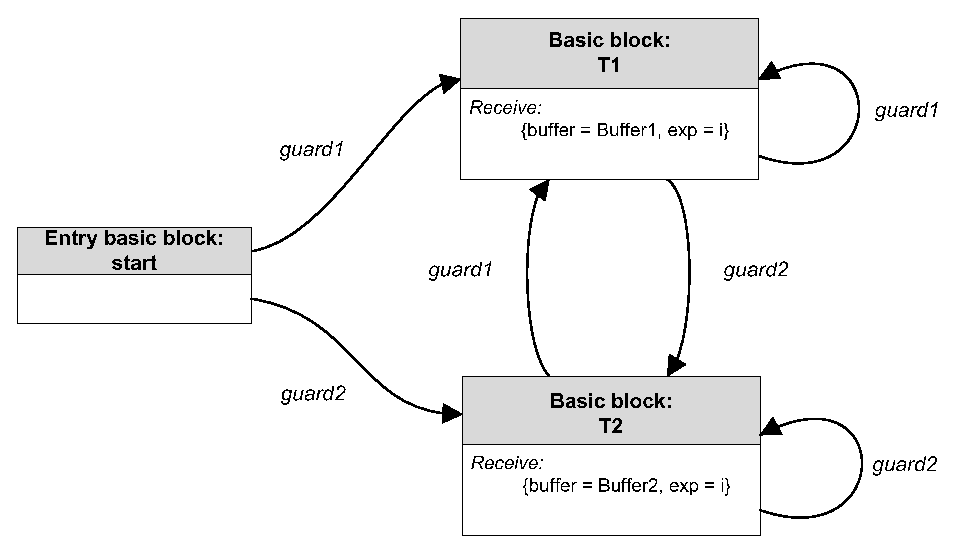
\includegraphics[scale=0.5]{translation/advancedissues/graphics/cffcfg.eps}
\caption{The CFG showing the control flow branch}
\label{fig:cffcfg}
\end{figure}

\subsubsection{Translating to an AST}

The CFG is then translated to the AST shown in Fig.~\ref{fig:cffast}. The \code{Process} node contains two blocks \code{T1} and \code{T2}. Taking a look at \code{T1} it contains a receive statement which has a pointer to \code{Buffer1} where the incoming messages are stored. The receive statement also contains a local variable \code{i} into which a message from the buffer is read. \code{T1} also contains two conditional statements; one holding the condition expression \code{guard1} and pointing to \code{T1}, and one holding the condition expression \code{guard2} and pointing to \code{T2}. The block \code{T2} is similar to \code{T1}.

\begin{figure}[b!]
\centering
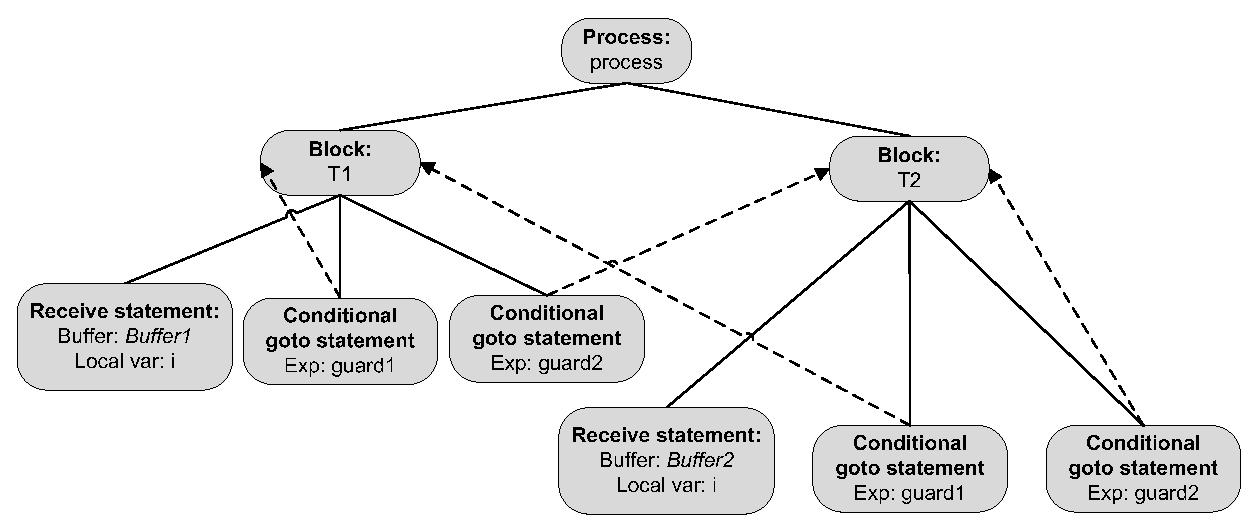
\includegraphics[scale=0.65]{translation/advancedissues/graphics/cffast.eps}
\caption{The AST showing the control flow branch}
\label{fig:cffast}
\end{figure}

\subsubsection{Translating to Erlang Source Code}
%In the phase from AST to EST things become a bit more complicated when buffers are involved as in this small example.
Next, we explain how control flow branches are handled when there are no buffers involved. In this section we omit the EST and only show the printed Erlang code. In Listing~\ref{list:cffnobuf} we see the code for \code{t1} generated from the AST (ignoring the receive statements) in Fig.~\ref{fig:cffast}.

\begin{figure}[h!]
\begin{verbatim}[style=erlangcode, caption=Generated Erlang code without receive statements, label=list:cffnobuf]
t1() -> 
    ...
    if
        Guard1 ->
            t1();
        Guard2 ->
            t2()
    end.
\end{verbatim}
\end{figure}


In the bottom of the function the guard expressions are evaluated, and jumps are made accordingly. Notice that if none of the guard expressions evaluate to \code{true} the program terminates. This is equivalent to the behaviour of the CPN model, in which this corresponds to none of the transitions, the process can proceed to, being enabled. Since we do not allow tokens on shared places or buffer places to be referred to in the guard expressions, the transitions cannot become enabled in the future.

This is code is generated for control flow branches when the goto statements points to blocks without receive statements. Generating Erlang code when there is a receive statement in one of the target blocks is a bit more complicated.

\paragraph{Goto a block with a receive statement.}
Jumping to the first block were the guard evaluates to \code{true} could introduce a deadlock in the program if that block contains a receive statement from a buffer that will never have an element added. For instance, in the ProPCPN model shown in fig.~\ref{fig:cffcpn}, it could be the case that both \figitem{guard1} and \figitem{guard2} evaluates to \code{true}. Assume that \figitem{Buffer1} is empty, and that there will never be added a token to it. Assume also that \figitem{Buffer2} already contains a token. If the program where to jump to the function corresponding to the transition \figitem{T1} the program would stop on the blocking receive expression. This is not desirable since \figitem{T2} is enabled in the CPN model, thus calling the function corresponding to \figitem{T2}, would not make the program stop.

The solution we have found is to only jump to a function with a receive expression if there is an element in the buffer. Since buffers are local to a process instance, the element will remain in the buffer until removed by that process instance. Thus it is guaranteed that the buffer element is still available when the function will be executed. We have introduced an explicit Erlang buffer module (found in appendix \ref{appsec:buffer}) with two additional operations:

\begin{itemize}
 \item The function \code{has\_element} can be used to determine if there is an element in the buffer. It does not change the state of the buffer. 
 \item The function \code{interrupt\_me} is used like a blocking receive call if the buffer is empty. The buffer will send a message with the atom literal \code{interrupt} when an element is added to the buffer.
\end{itemize}

\begin{figure}[h!]
\begin{verbatim}
    t1(Env) -> 
    ...
    t1_loop(Env).

t1_loop(Env) -> 
    Env#environment.buffer_1 ! has_element,
    receive 
        Buffer_1_has_elements -> 
            Buffer_1_has_elements
    end,
    Env#environment.buffer_2 ! has_element,
    receive 
        Buffer_2_has_elements -> 
            Buffer_2_has_elements
    end,
    if
        Guard1, Buffer_1_has_elements ->
            t1(Env); 
        Guard2, Buffer_2_has_elements ->
            t2(Env);
        true ->
            if
                not Buffer_1_has_elements ->
                    Env#environment.buffer_1 ! interrupt_me;
            end,       
            if       
                not Buffer_2_has_elements ->
                    Env#environment.buffer_2 ! interrupt_me
            end
    end,
    receive 
        interrupt -> 
            t1_loop(Env)
    end.
\end{verbatim}
\end{figure}


Listing~\ref{list:cffwithbuf} shows how \code{has\_element} and \code{interrupt\_me} are used in the generated code. The function \code{t1\_loop} line 5-34 is used to decide which function to call next. In line 6-15 the \code{has\_element} operation is used on \code{Buffer1} and \code{Buffer2} and bound to variables. In line 17-18 we see how the function \code{t1} is called if \code{Guard1} evaluates to \code{true} and the buffer has an element. The \code{true} branch in line 21-29 is used if no function is available, i.e., none of the above guards evaluates to \code{true} or the buffers had no elements. This means, that until one of the buffers receives an element, none of the functions can be called. For this reason, it is requested that all the buffers without elements make an interrupt when an element becomes available. Finally, in line 31-34 \code{t1} is blocked until an interrupt is received from one of the buffers, in which case \code{t1\_loop} is called again.

\chapter{Implementing the Translation}
\label{chap:tool}
In this chapter we first present some of the technologies used in this project. We then present the implementation of the translation from a ProPCPN model to Erlang code. Finally, we present a validation of the generated code from the producer-consumer ProPCPN model.

\section{The Eclipse Platform}
The open source project Eclipse \cite{RefWorks:86} is probably best known for the integrated development environment (IDE), which is used by many programmers to write programs in. Eclipse is based on Java and offers a lot of tools and frameworks for developing applications. The Eclipse platform has a plug-in based structure. The platform provides a core framework and services upon which plug-ins can be created. A plug-in is a piece of code that adds new functionality to the platform. Plug-ins can be used, e.g., to add support for new programming languages to the Eclipse IDE, or integrate a new way of searching for resources in the workspace.

Commonly used services and frameworks are built into the Eclipse platform. These include a standard workbench user interface, and a project model for managing resources. The Rich Client Platform \cite{RefWorks:83} allows the developer to use the Eclipse platform to create stand-alone applications that can be exported to multiple platforms. An example of a Rich Client Platform application is the ASAP tool \cite{RefWorks:92} which we mentioned earlier.

\subsection{The Eclipse Modeling Framework}
The Eclipse Modeling Framework (EMF) \cite{RefWorks:85} is a framework for creating object or domain models based on a structured data model. The framework allows the programmer to build a model, e.g., specified as a collection of Java interface. The framework can then produce a set of Java classes for the model, but also a viewer and a basic editor which can be plugged in the Eclipse IDE.

In this project we have built three models in the EMF framework, one for the structure of the control flow graph, one for the abstract syntax tree, and one for the Erlang syntax tree. We use EMF to produce Java classes and editors for the structures which enable us to visualise the result of the phases in the translation.

The EMF framework offers a way of extending an existing model by using \emph{adapters}. Adapters can be attached to an existing interface and allow it to support additional interfaces without subclassing it. The ASAP tool contains an EMF model of a CPN model which we have used in the translation. We extended the behaviour of the model using adapters in order to be able to attach the decorations made in the decoration phase of the translation. 


\section{CPN Tools}
CPN Tools \cite{RefWorks:87} is a tool for editing, simulating, and doing state space and performance analysis of CPN models. The ProPCPN models presented in this thesis are constructed using CPN Tools. In Fig.~\ref{fig:cpntools} we show a screenshot of the producer-consumer model in CPN Tools. The user works directly with the graphical representation of the model, e.g., a transition can be drawn using the rectangle in the tool box shown in the upper right corner of Fig.~\ref{fig:cpntools}. The model is being checked for errors continuously to assist the user in the construction of CPN models. ProPCPNs, being a subclass of CPNs, can be created and analysed in CPN Tools just like any other CPN model. 

\ignore{In the current version it is the modellers responsibility that the model is in fact a ProPCPN model.}   

\begin{figure}[b!]
\centering
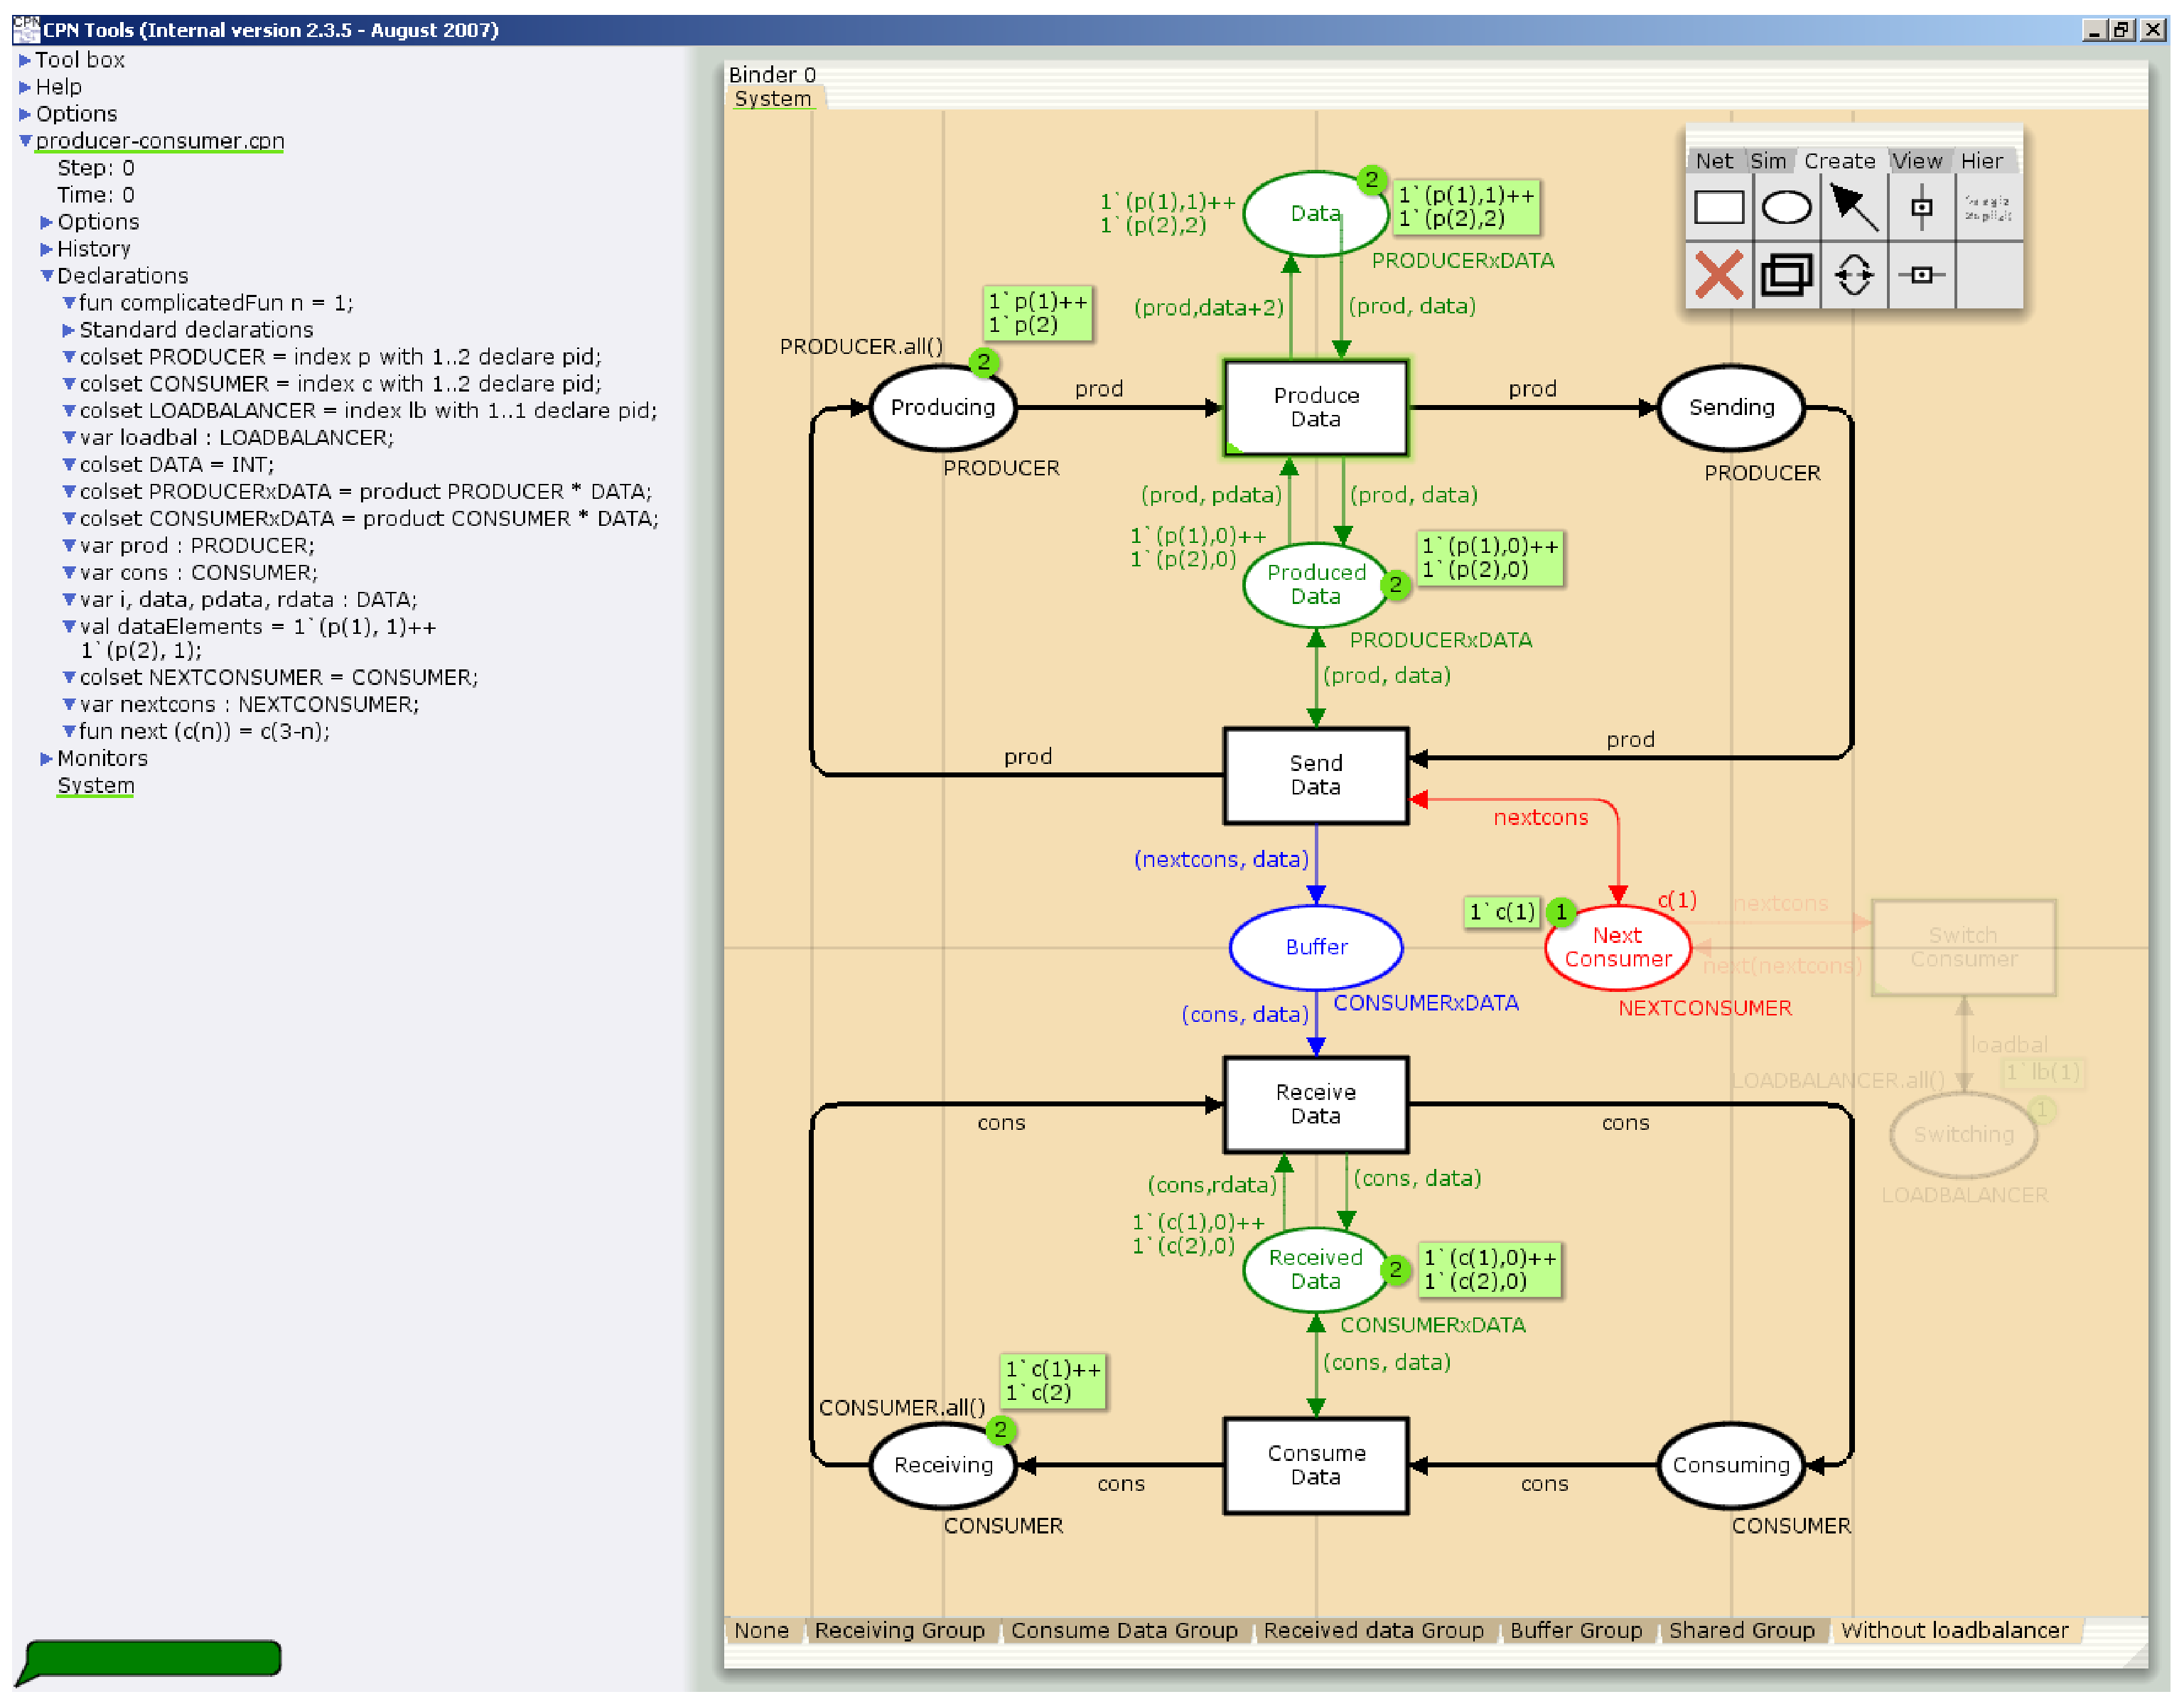
\includegraphics[width=\textwidth]{techniques_and_tool/graphics/CPNTools.eps}
\caption{The producer-consumer model in CPN Tools}
\label{fig:cpntools}
\end{figure}

\section{The Implemention of the Translation}
\label{sec:owntool}
Our implementation of the translation is written as a plug-in to the ASAP tool. By making a plug-in to ASAP we can make use of the EMF CPN model and the CPN importer which makes it possible to import CPN models created in CPN Tools into the workspace. In the following we walk through the most important parts of the tool. Eclipse user would find the graphical user interface (see Fig.~\ref{fig:newproject}) familiar, since it looks very similar to the standard Eclipse IDE.

\begin{figure}[h!]
\centering
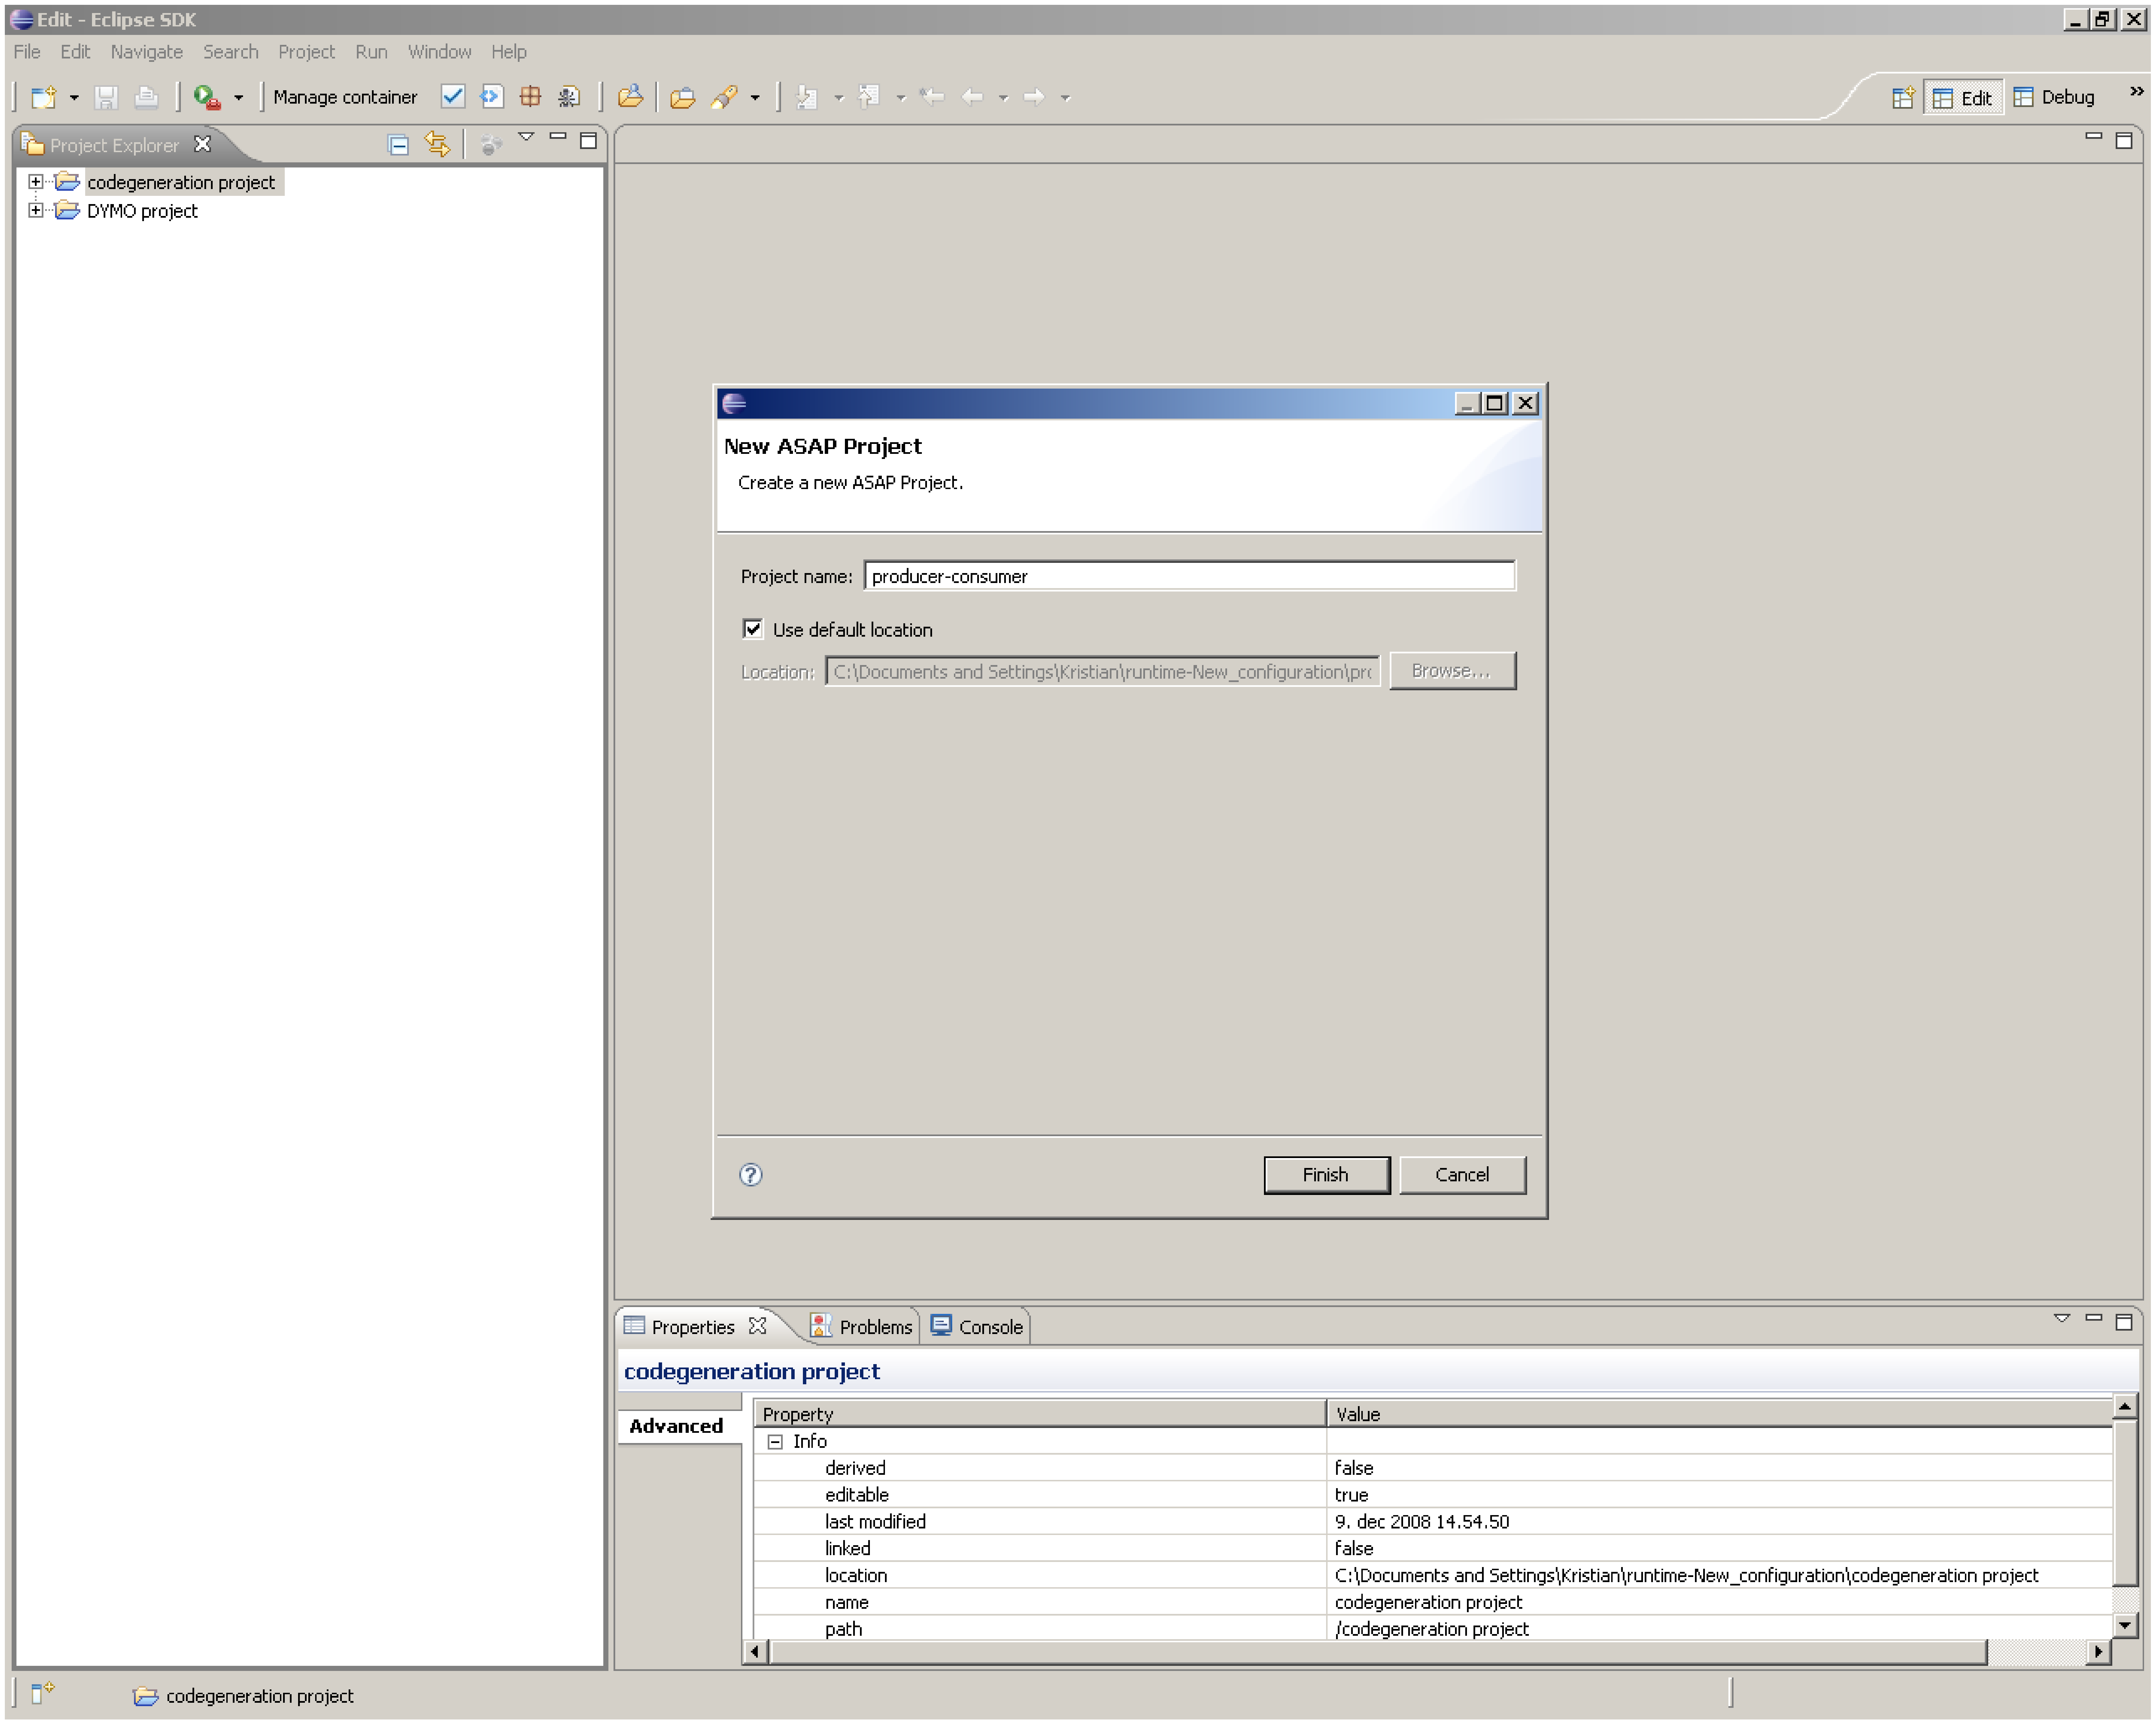
\includegraphics[width=\textwidth]{techniques_and_tool/graphics/newproject.eps}
\caption{The new ASAP project wizard}
\label{fig:newproject}
\end{figure}

To the left we see the \emph{project explorer}. To create a new project in the project explorer go to the \textbf{File} menu and choose \textbf{New} $\rightarrow$ \textbf{ASAP project}. The new ASAP project wizard will appear which is shown in Fig.~\ref{fig:newproject}. When the \textbf{Finish} button is pressed the wizard creates an ASAP project with the four folders \code{jobs}, \code{models}, \code{queries}, and \code{reports}. By right-clicking on the \textbf{models} folder it is possible to import models created in CPN Tools. The models are imported using the wizard shown in Fig.~\ref{fig:importcpn}. When the \textbf{Finish} button is pressed the CPN model is imported into the project and the folder \textbf{models} now contain the CPN model in a \code{.model} file which is an EMF model representation of the CPN model.

\begin{figure}[h!]
\centering
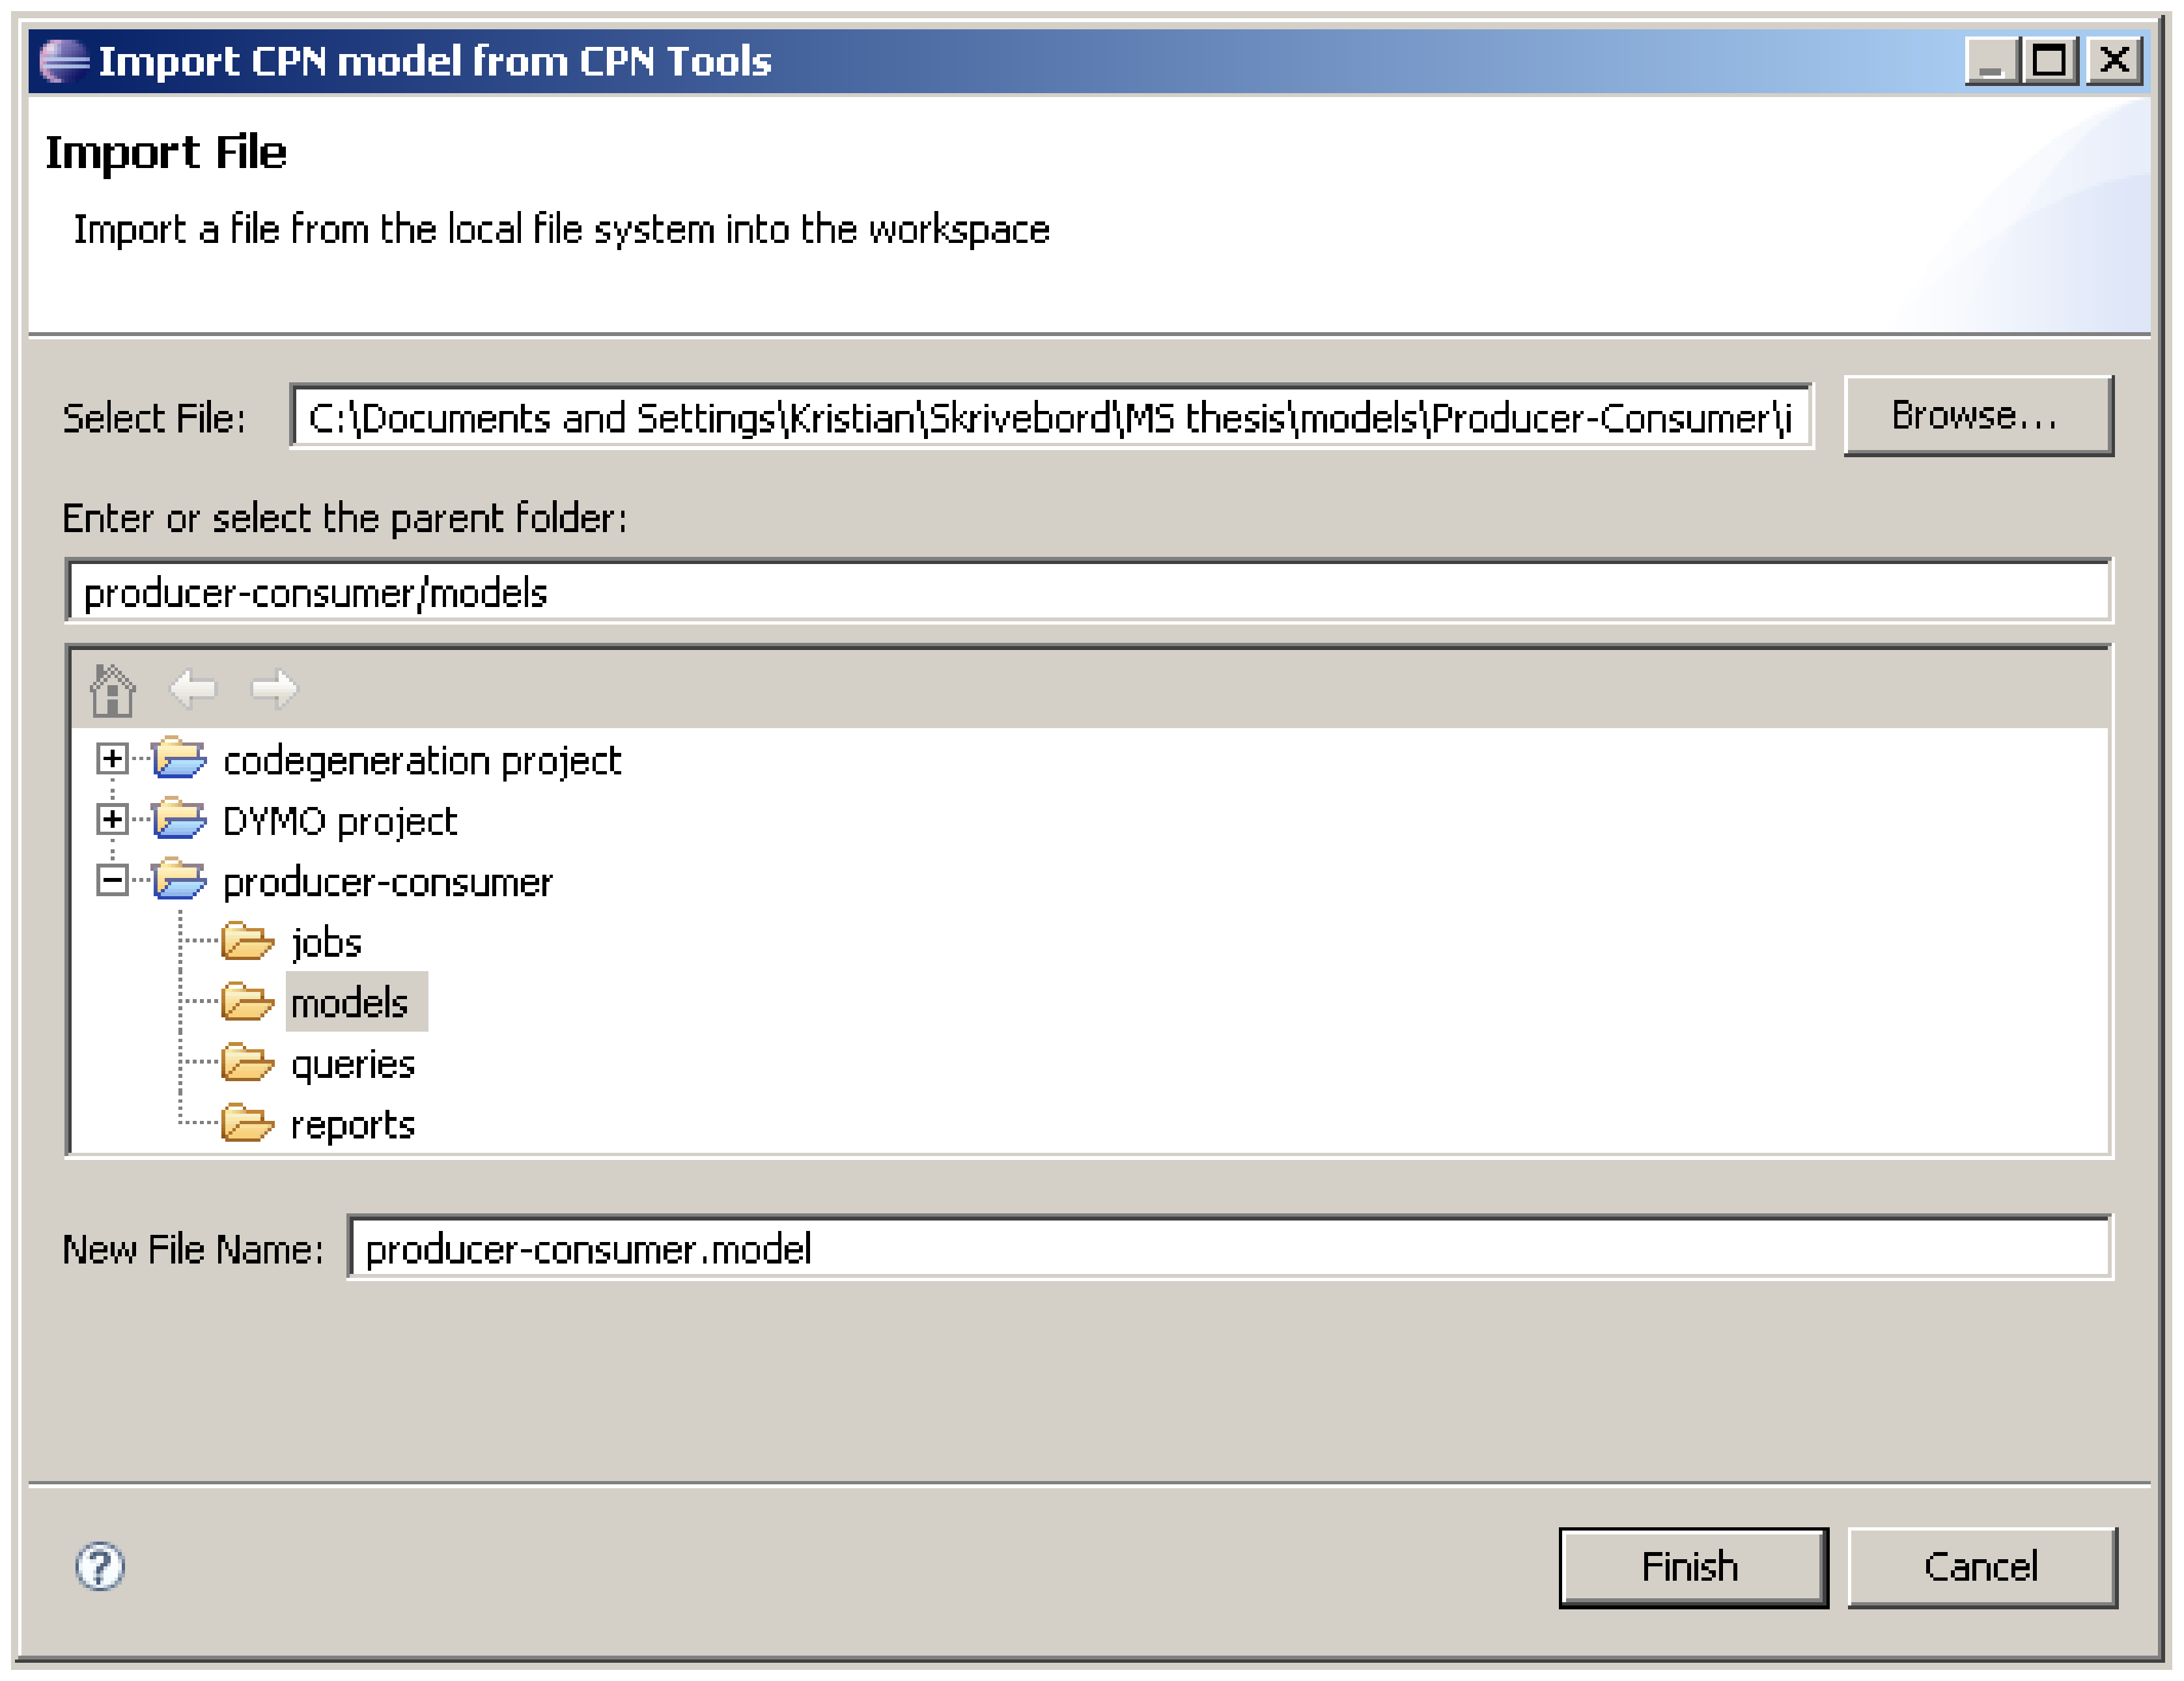
\includegraphics[scale=0.2]{techniques_and_tool/graphics/importcpn.eps}
\caption{The CPN model importer}
\label{fig:importcpn}
\end{figure}

We have added the possibility of right-clicking on a \code{.model} file, and choose \emph{Erlang code generation} which starts the wizard shown in Fig.~\ref{fig:cg1}. In this wizard the folder which will contain the generated code is given a name.

\begin{figure}[b!]
\centering
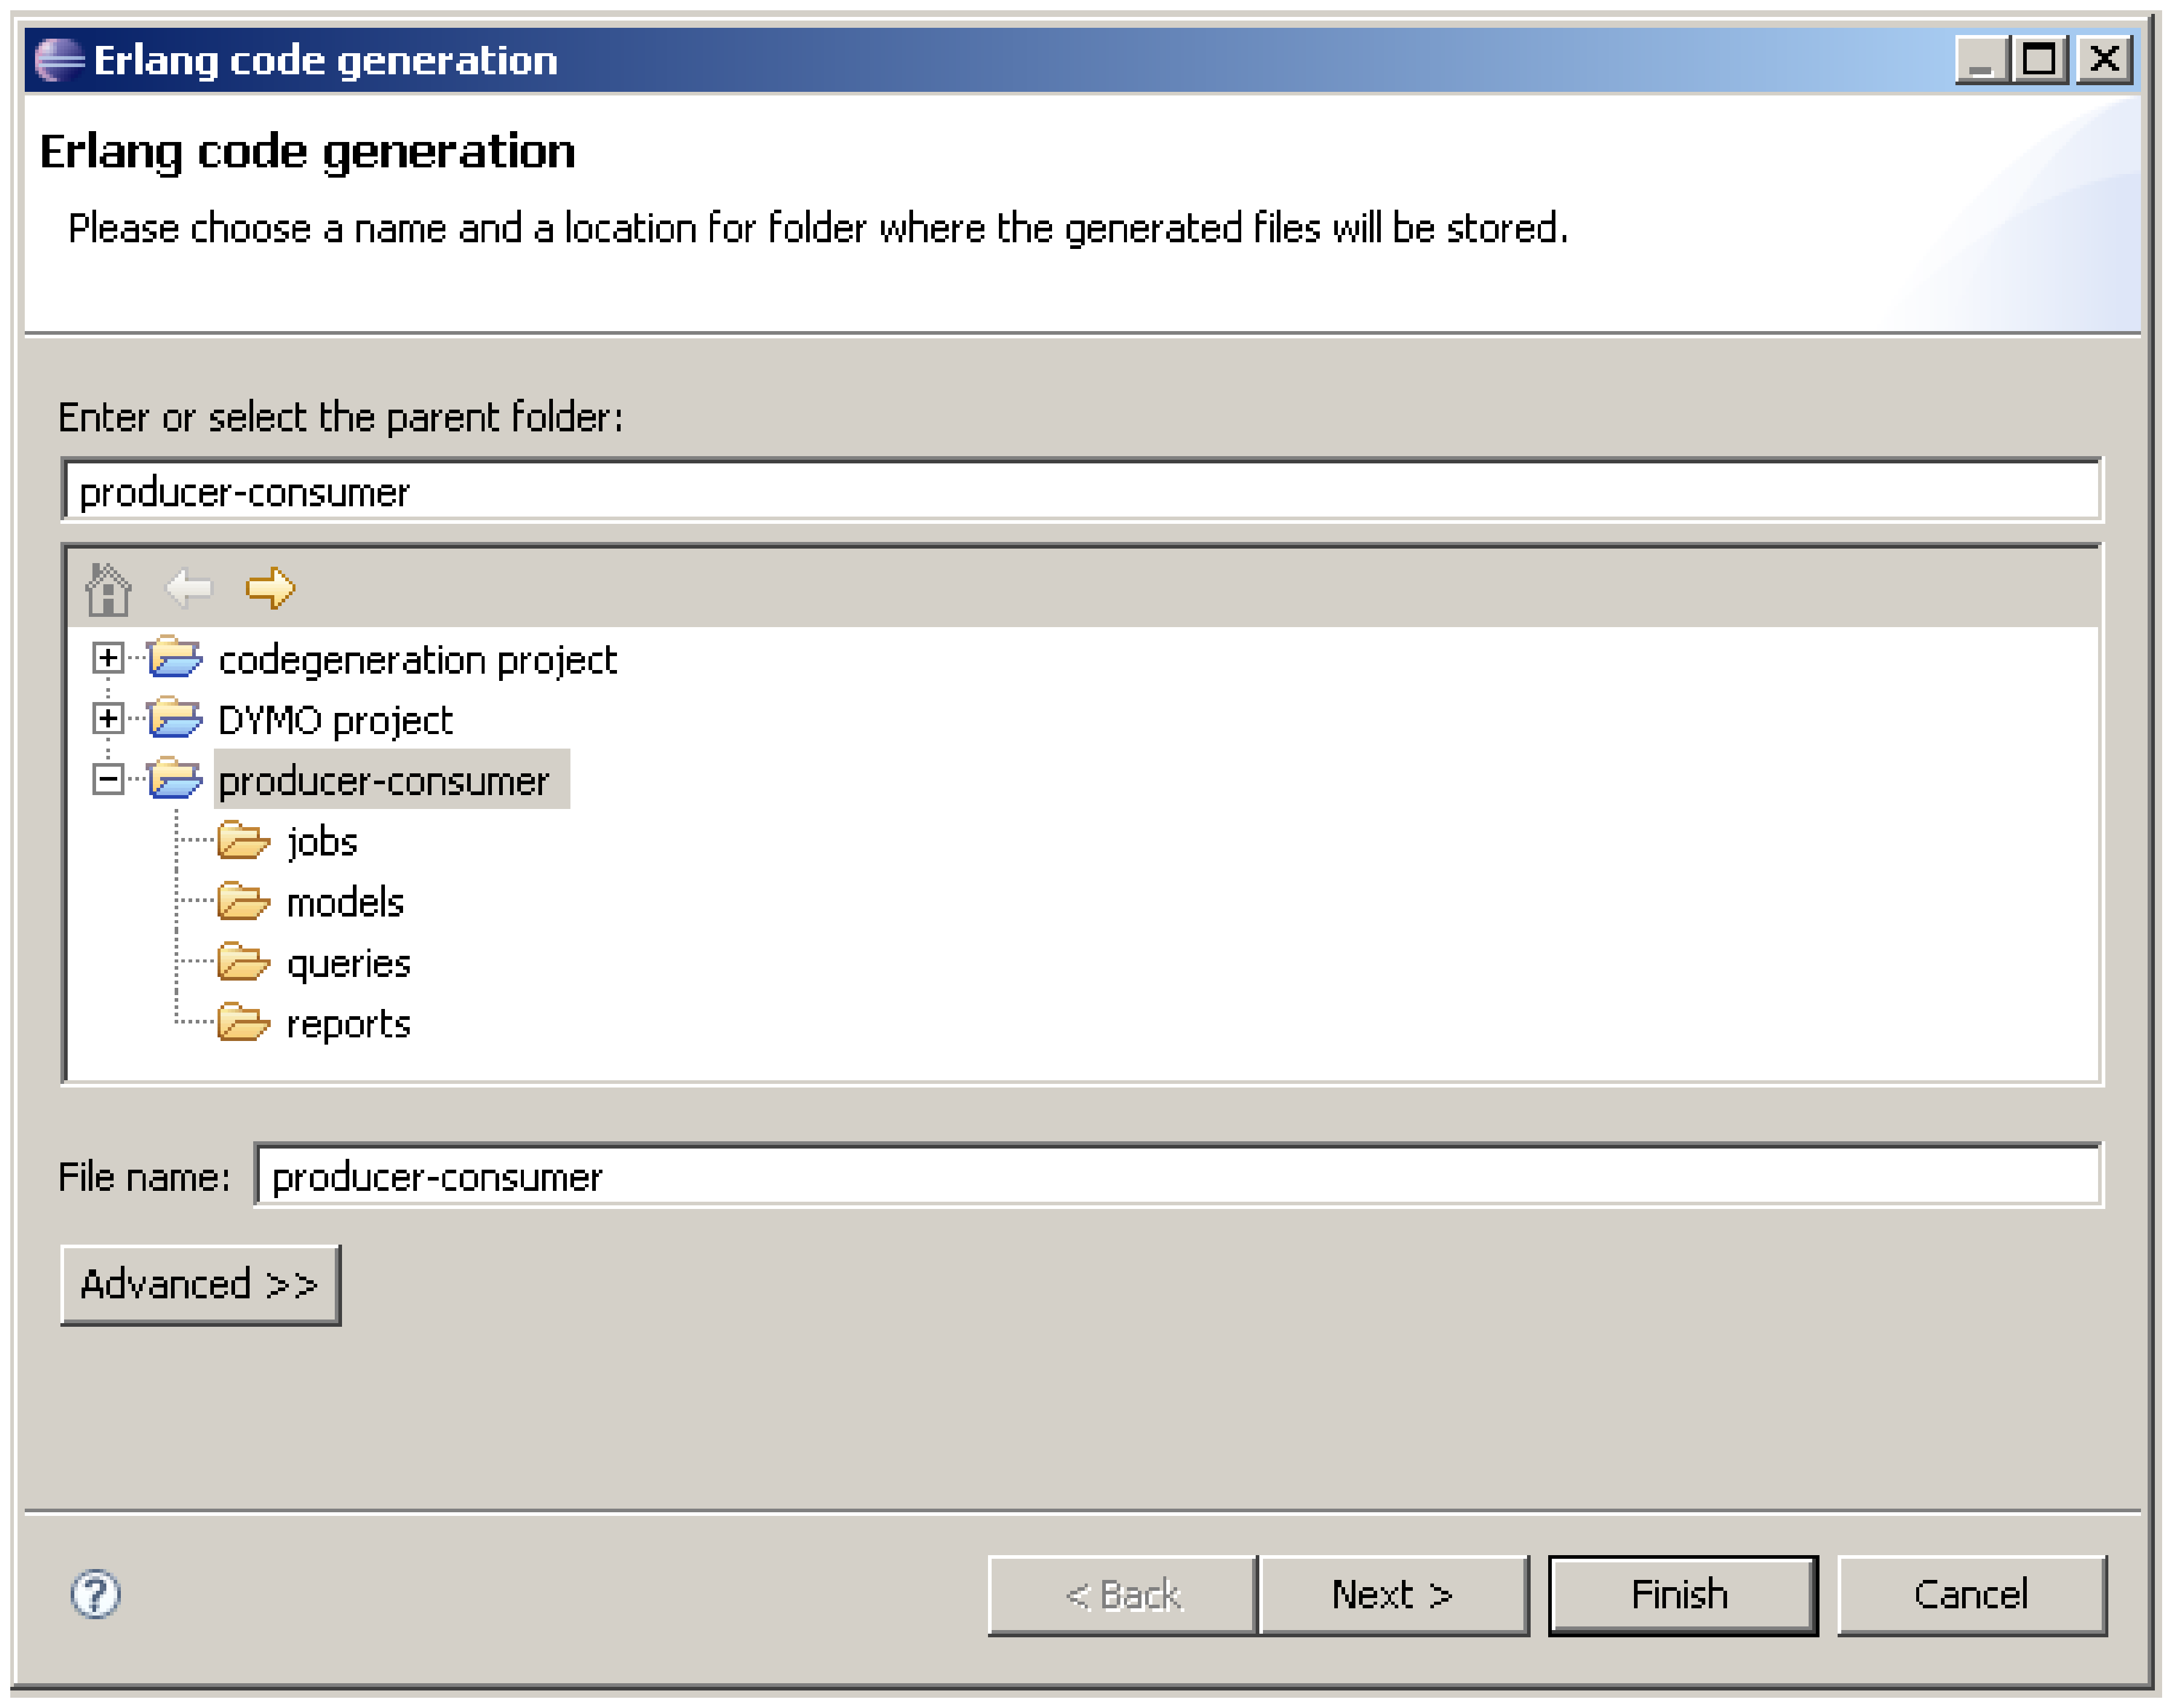
\includegraphics[scale=0.2]{techniques_and_tool/graphics/cg1.eps}
\caption{The code generator wizard step 1}
\label{fig:cg1}
\end{figure}

When pressing the \textbf{Next} button the screen in Fig.~\ref{fig:cg2} is shown. Here the user is able to choose which files should be generated by using the four check boxes in the top of the wizard. Below the CPN model to generate code from is chosen. When the \textbf{Finish} button is pressed the chosen files are generated and put into a folder as shown in Fig.~\ref{fig:cgprojectexplorer}.

\begin{figure}[h!]
\centering
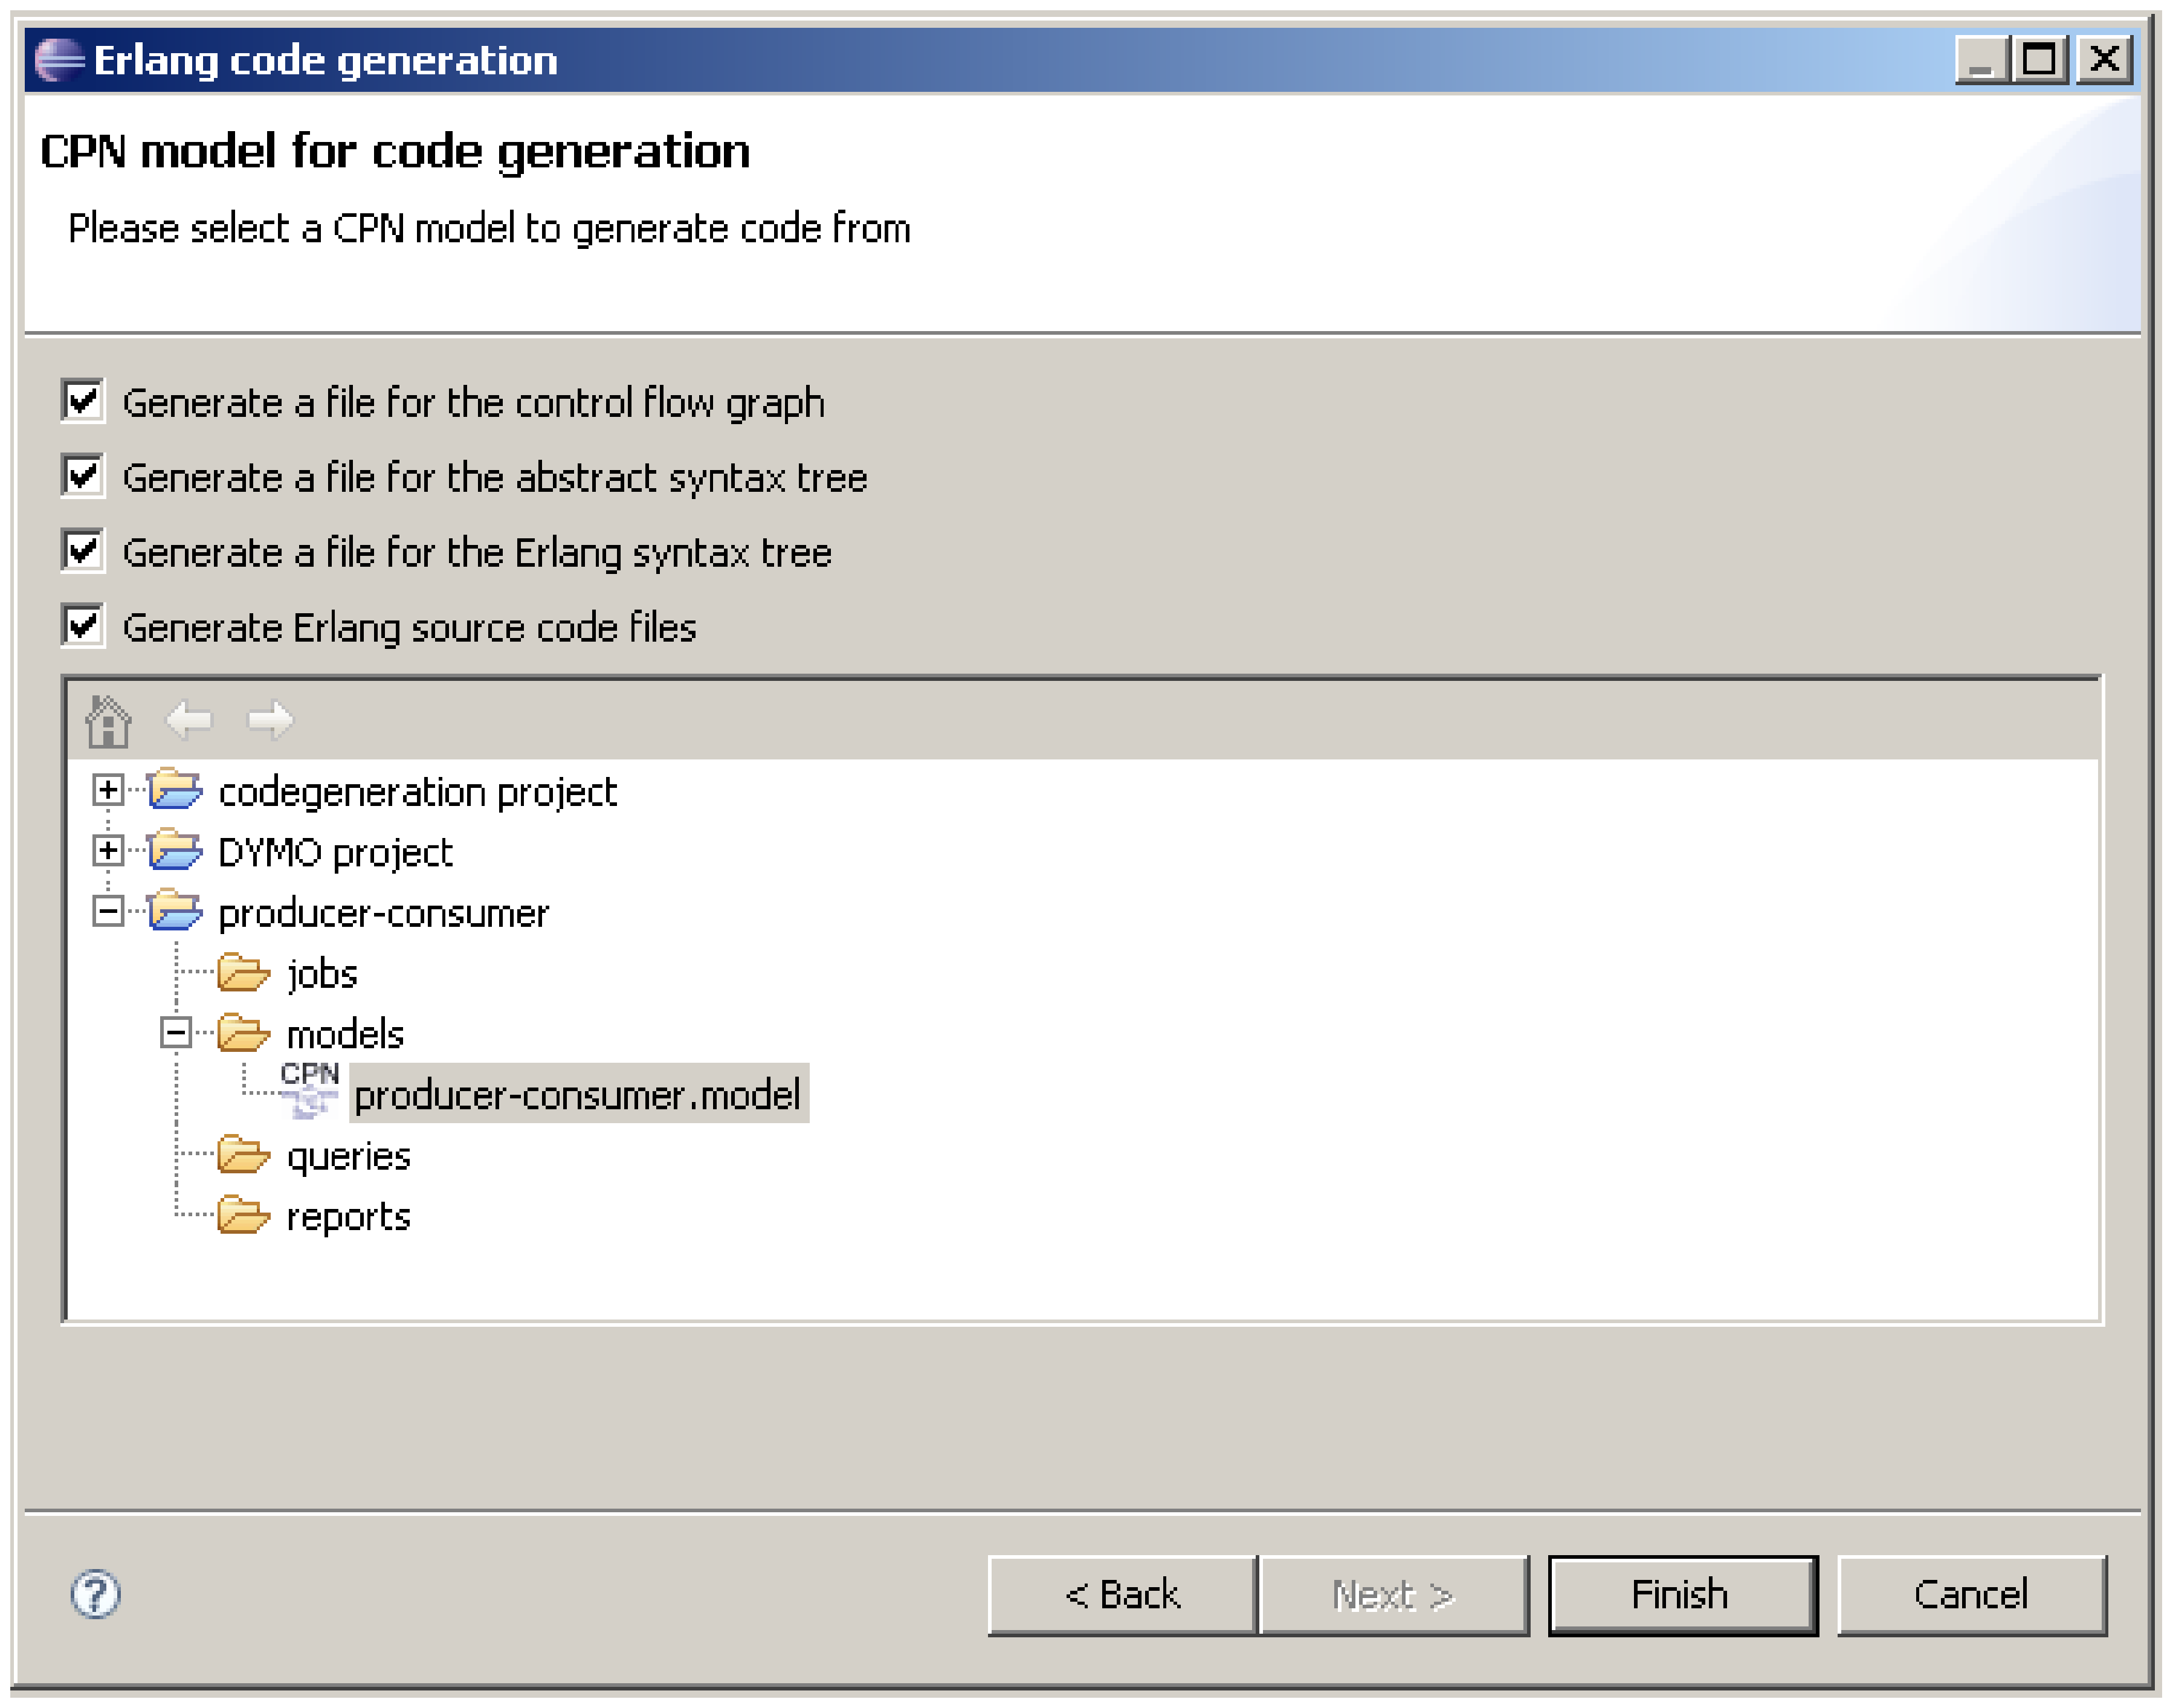
\includegraphics[scale=0.2]{techniques_and_tool/graphics/cg2.eps}
\caption{The code generator wizard step 2}
\label{fig:cg2}
\end{figure}

\begin{figure}[b!]
\centering
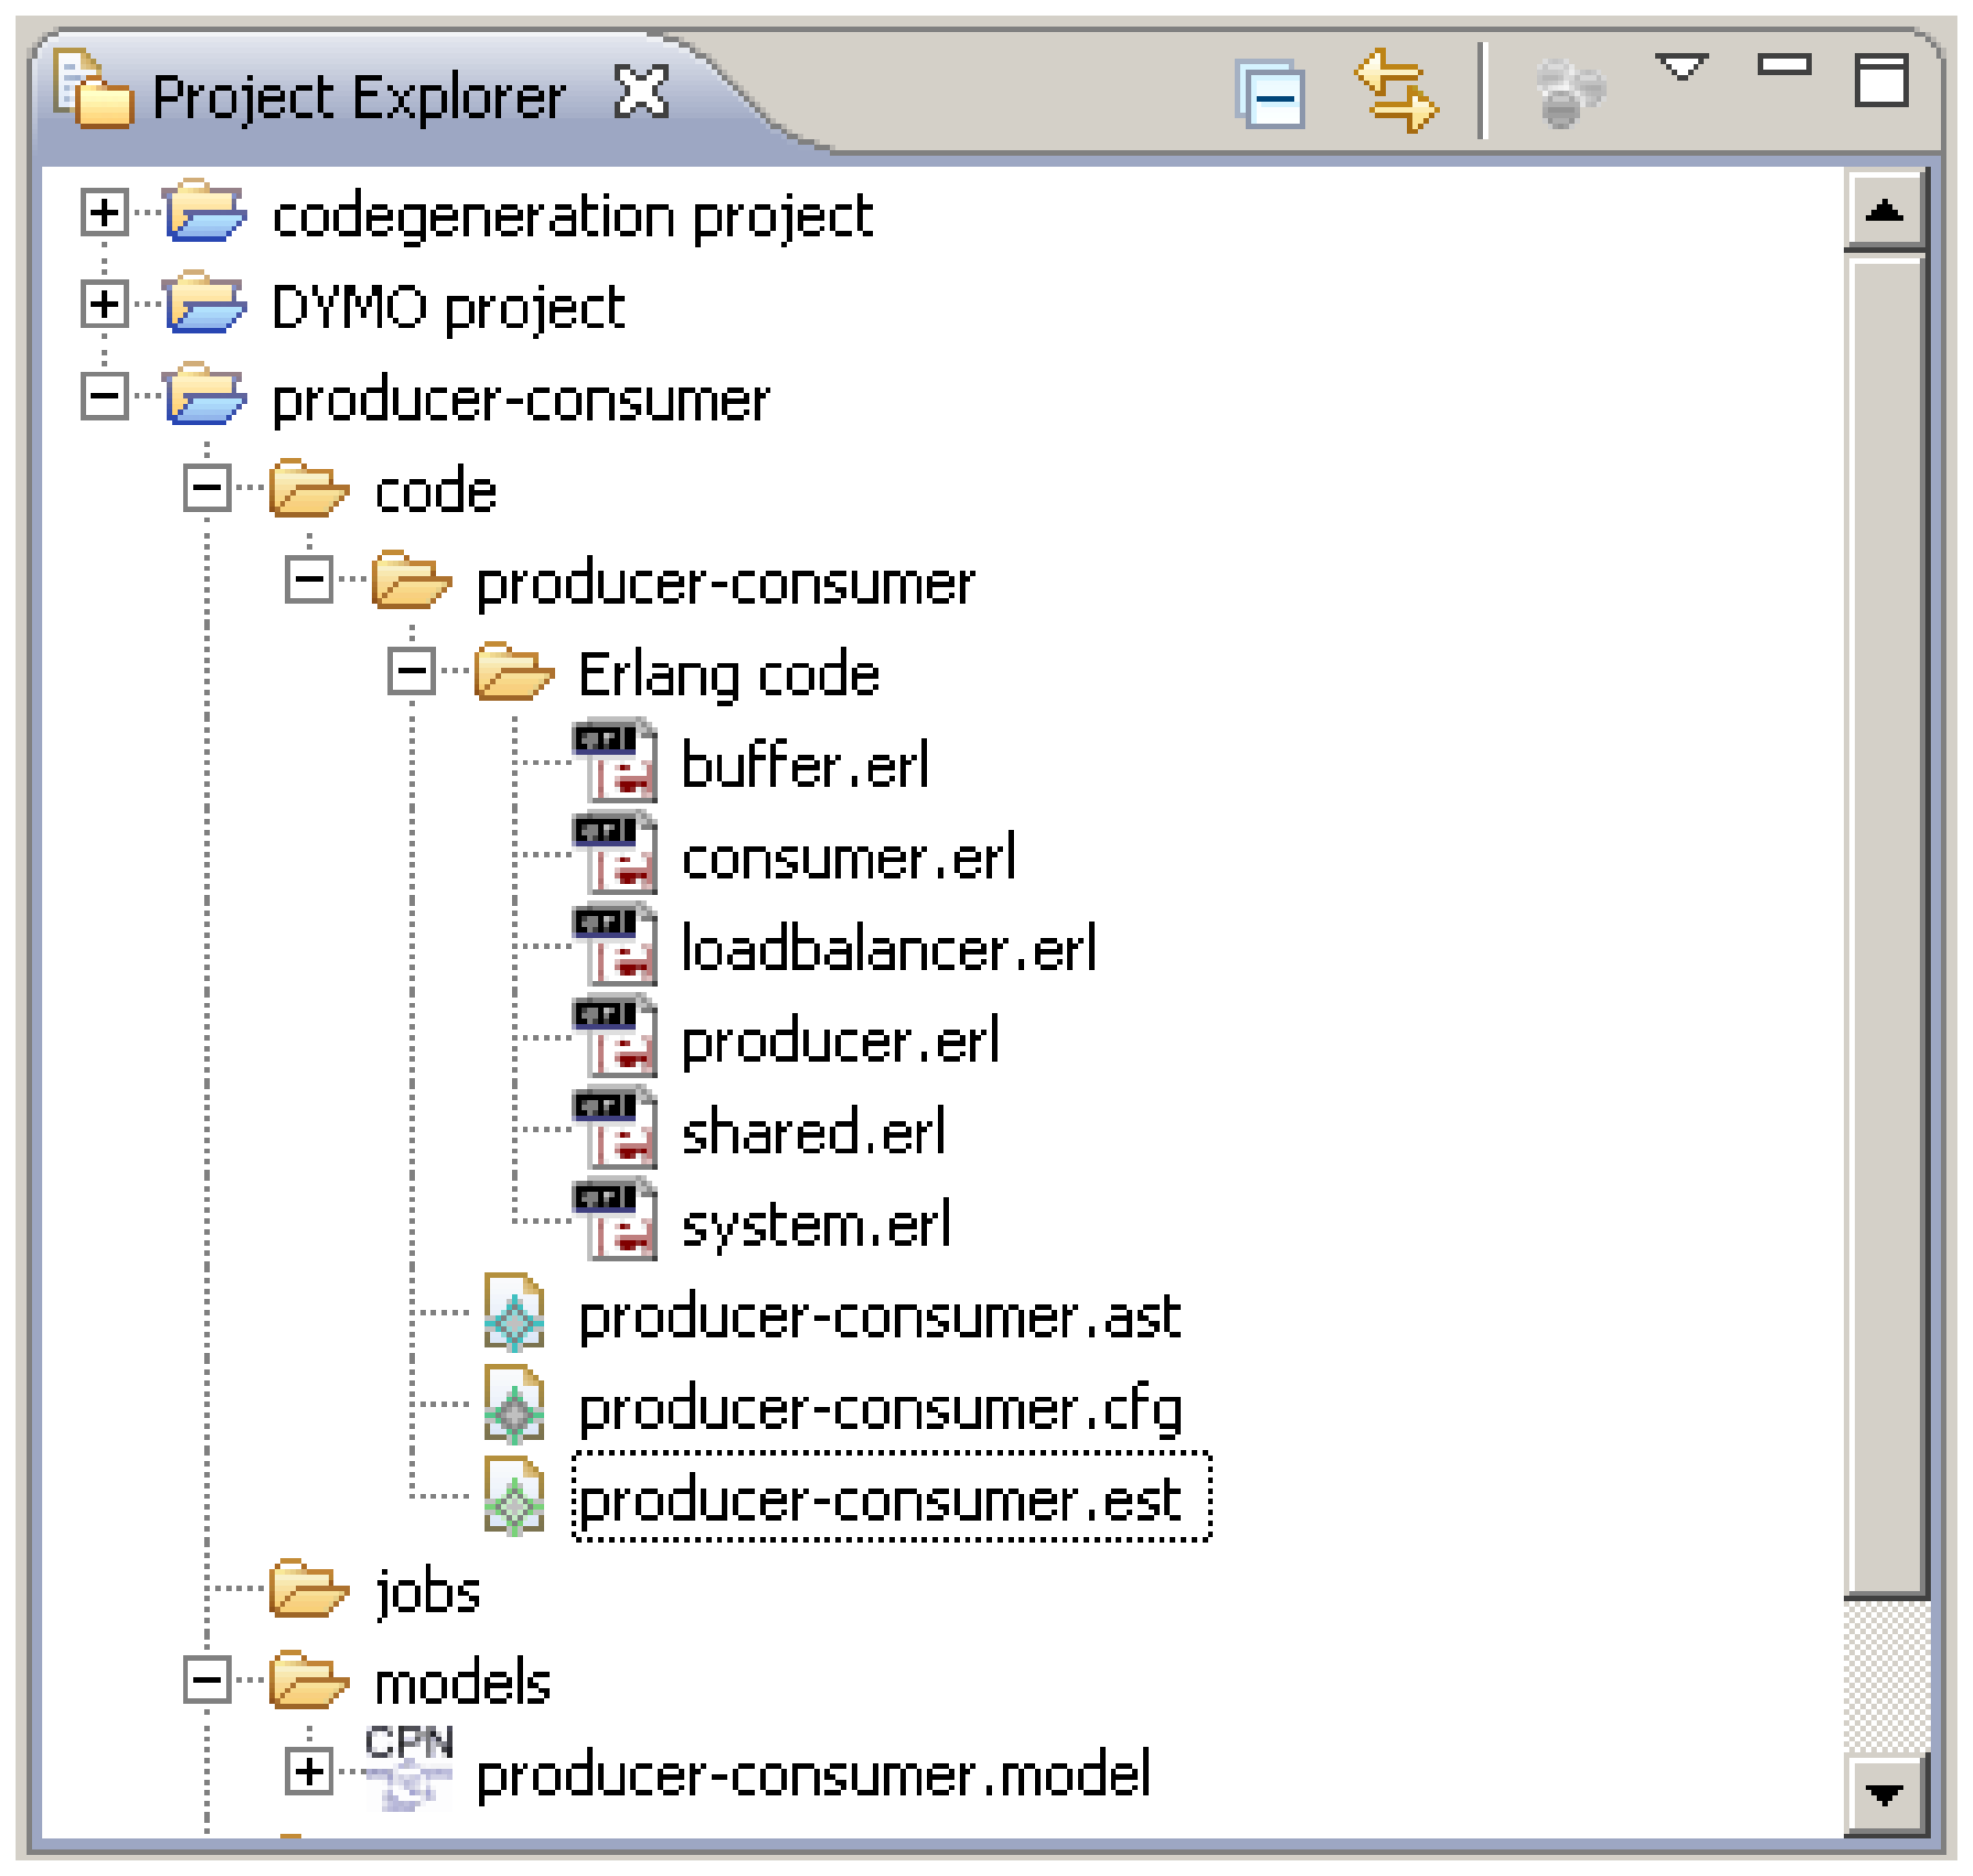
\includegraphics[scale=0.2]{techniques_and_tool/graphics/cgprojectexplorer.eps}
\caption{The project explorer after running the code generator wizard}
\label{fig:cgprojectexplorer}
\end{figure}

In the following we describe the generated abstract syntax tree (AST) from the producer-consumer system, which is represented as an EMF model. The control flow graph and the Erlang syntax tree are visualised in a similar way as the AST. The tree representation is shown in the tool, which can be used to inspect the different phases of the translation. In section \ref{sec:validateprodcons} we take a closer look at the generated code.

%\subsection{The EMF Control Flow Graph}
%In Fig.~\ref{fig:cgcfg} we find part of the generated CFG. We see that three process nodes are created; one for the producer, one for the consumer, and one for the load-balancer. We also see the global variable \code{Next Consumer}. We have unfolded the producer process, and we see that it contains three basic blocks: \code{Send Data}, \code{Produce Data} and \code{start}. Taking a closer look at the basic block \code{Produce Data} we see that it contains a read from, and a write to, the process variables \code{Data} and \code{PData}. The edge in the control flow graph from the basic block \code{Produce Data} and \code{Send Data} is represented in the basic block condition pair.
%
%\begin{figure}
%\centering
%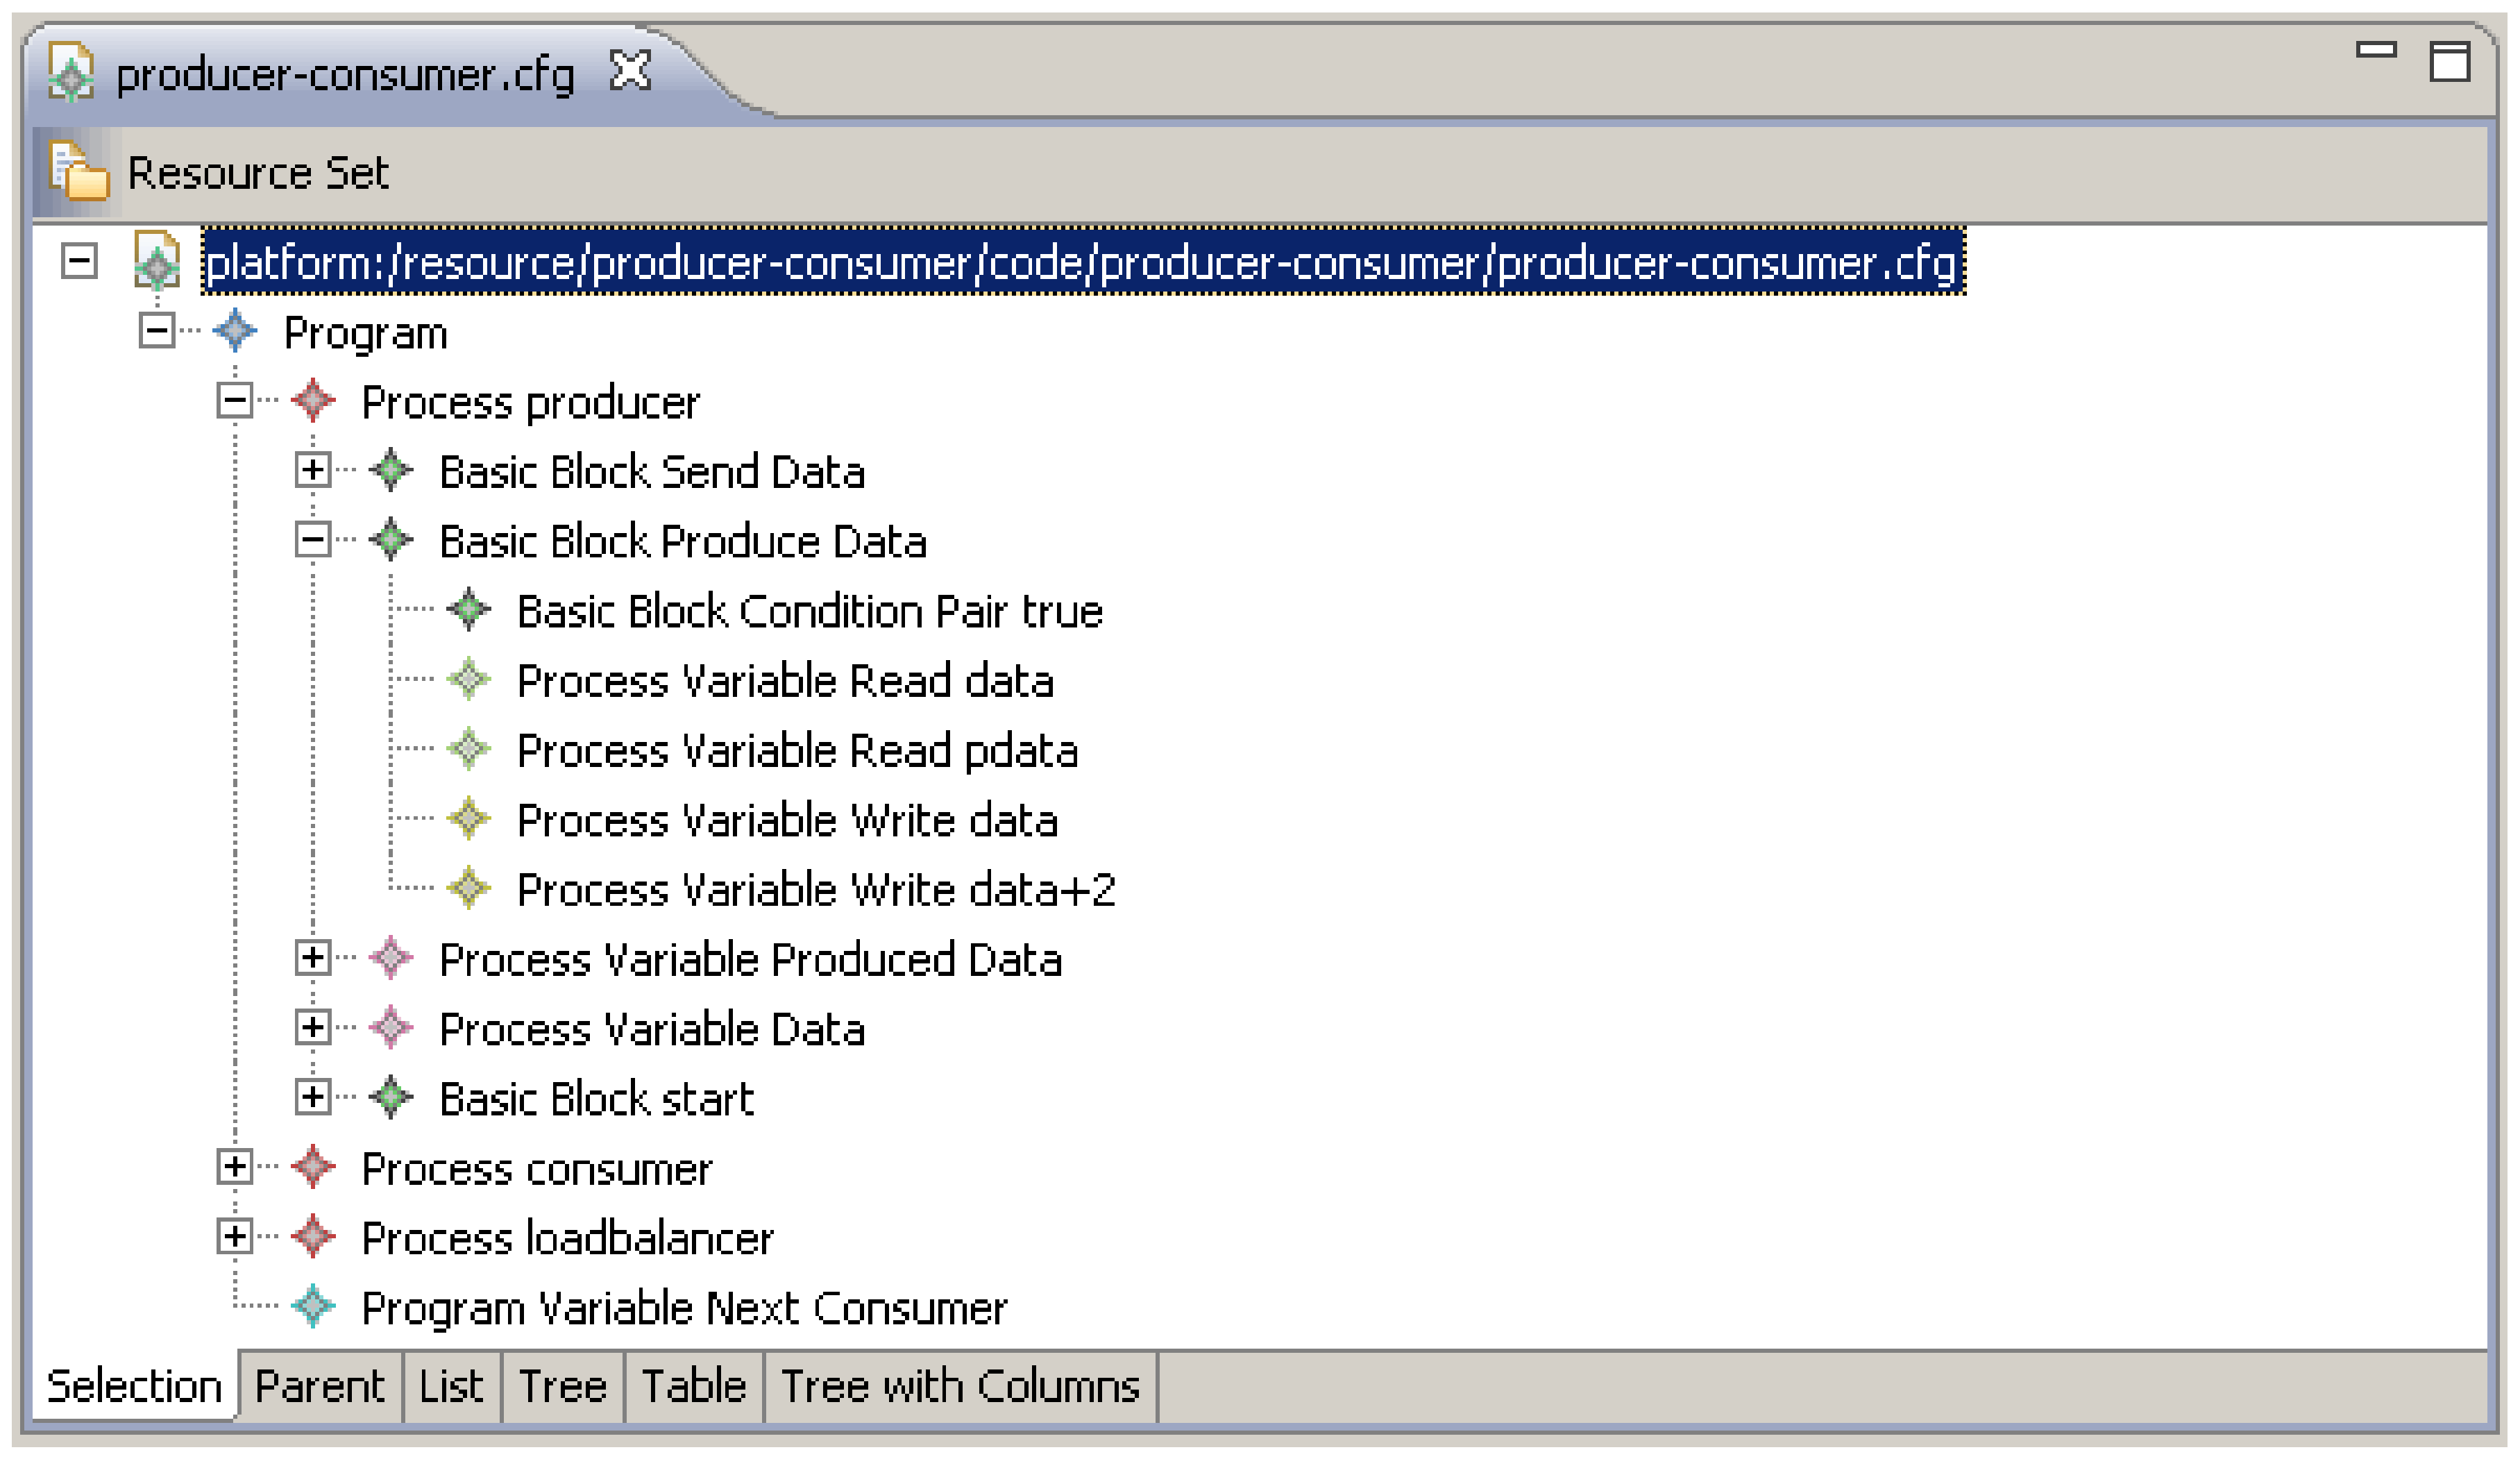
\includegraphics[scale=0.2]{techniques_and_tool/graphics/cfg.eps}
%\caption{The generated Control Flow Graph (CFG)}
%\label{fig:cgcfg}
%\end{figure}

\subsection{The EMF Abstract Syntax Tree}
In Fig.~\ref{fig:cgast} we show part of the generated AST. It contains the three processes: \code{producer}, \code{consumer} and \code{loadbalancer}. We see, that the initial expression of the global variable \code{Next Consumer} has been extracted. The initial expression is the integer constant \code{1} for \code{producer} instance one, and the integer constant \code{2} for producer instance two. Taking a closer look at the block \code{Produce Data} we see that two local variable declarations have been created. These are used in the read and write statements, e.g., we see the read statement where the value of the process variable \code{Data} is bound to the local variable declaration \code{data}. In the end of the block we see an unconditional goto statement.

\begin{figure}[b!]
\centering
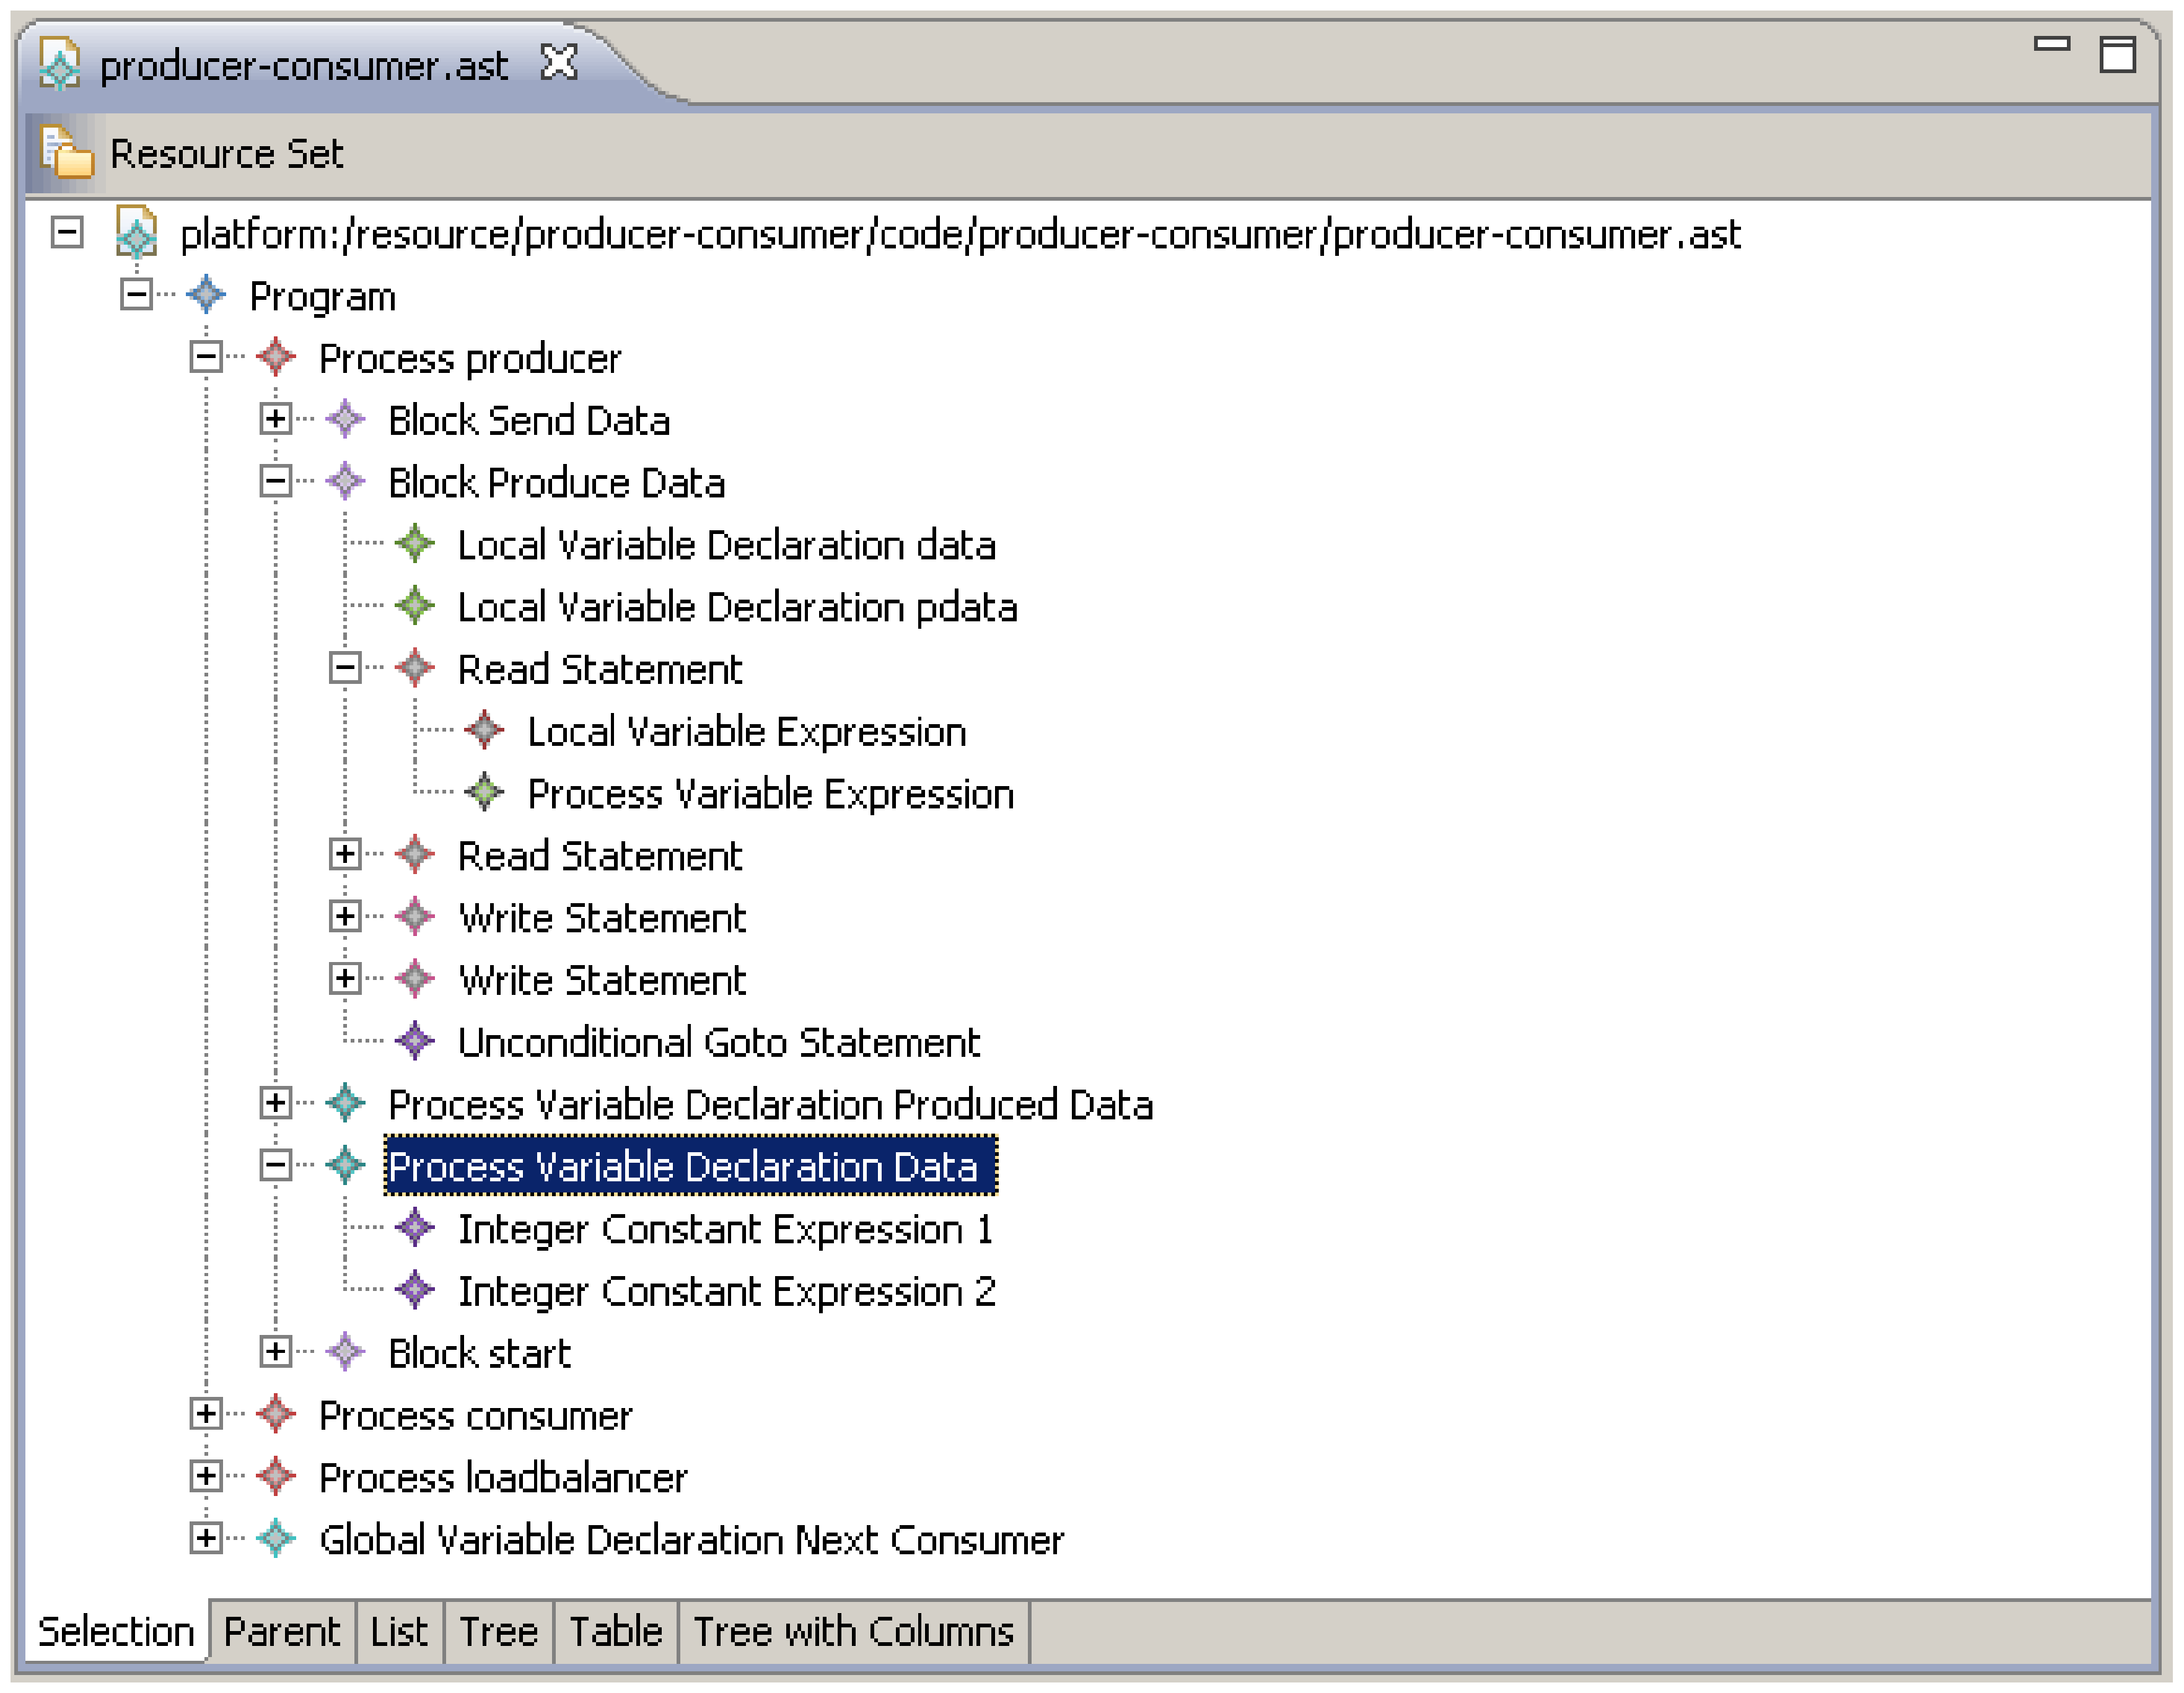
\includegraphics[scale=0.2]{techniques_and_tool/graphics/ast.eps}
\caption{The generated Abstract Syntax Tree (AST)}
\label{fig:cgast}
\end{figure}

%\subsection{The EMF Erlang Syntax Tree}
%In Fig.~\ref{fig:cgast} part of the EST is shown. In addition to the three module declarations for the producer, consumer and load-balancer, we see a system module and a shared module. The system module is responsible for spawning the process instances, and the shared module is used to share data as explained in \ref{TODO}. The module declaration for the producer is shown in some detail. We see the export attribute responsible for exporting the start function, and we also see the record declaration for the environment. It further more contains the three functions: \code{start}, \code{send\_data}, and \code{produce\_data}. Taking a closer look at the function declaration for \code{produce\_data}, we see the \code{Env} variable which is the argument to the function. We also see the match expression where the value of data is read from the environment. In the end of the function we see an application expression where the function \code{send\_data} is called.
%
%\begin{figure}
%\centering
%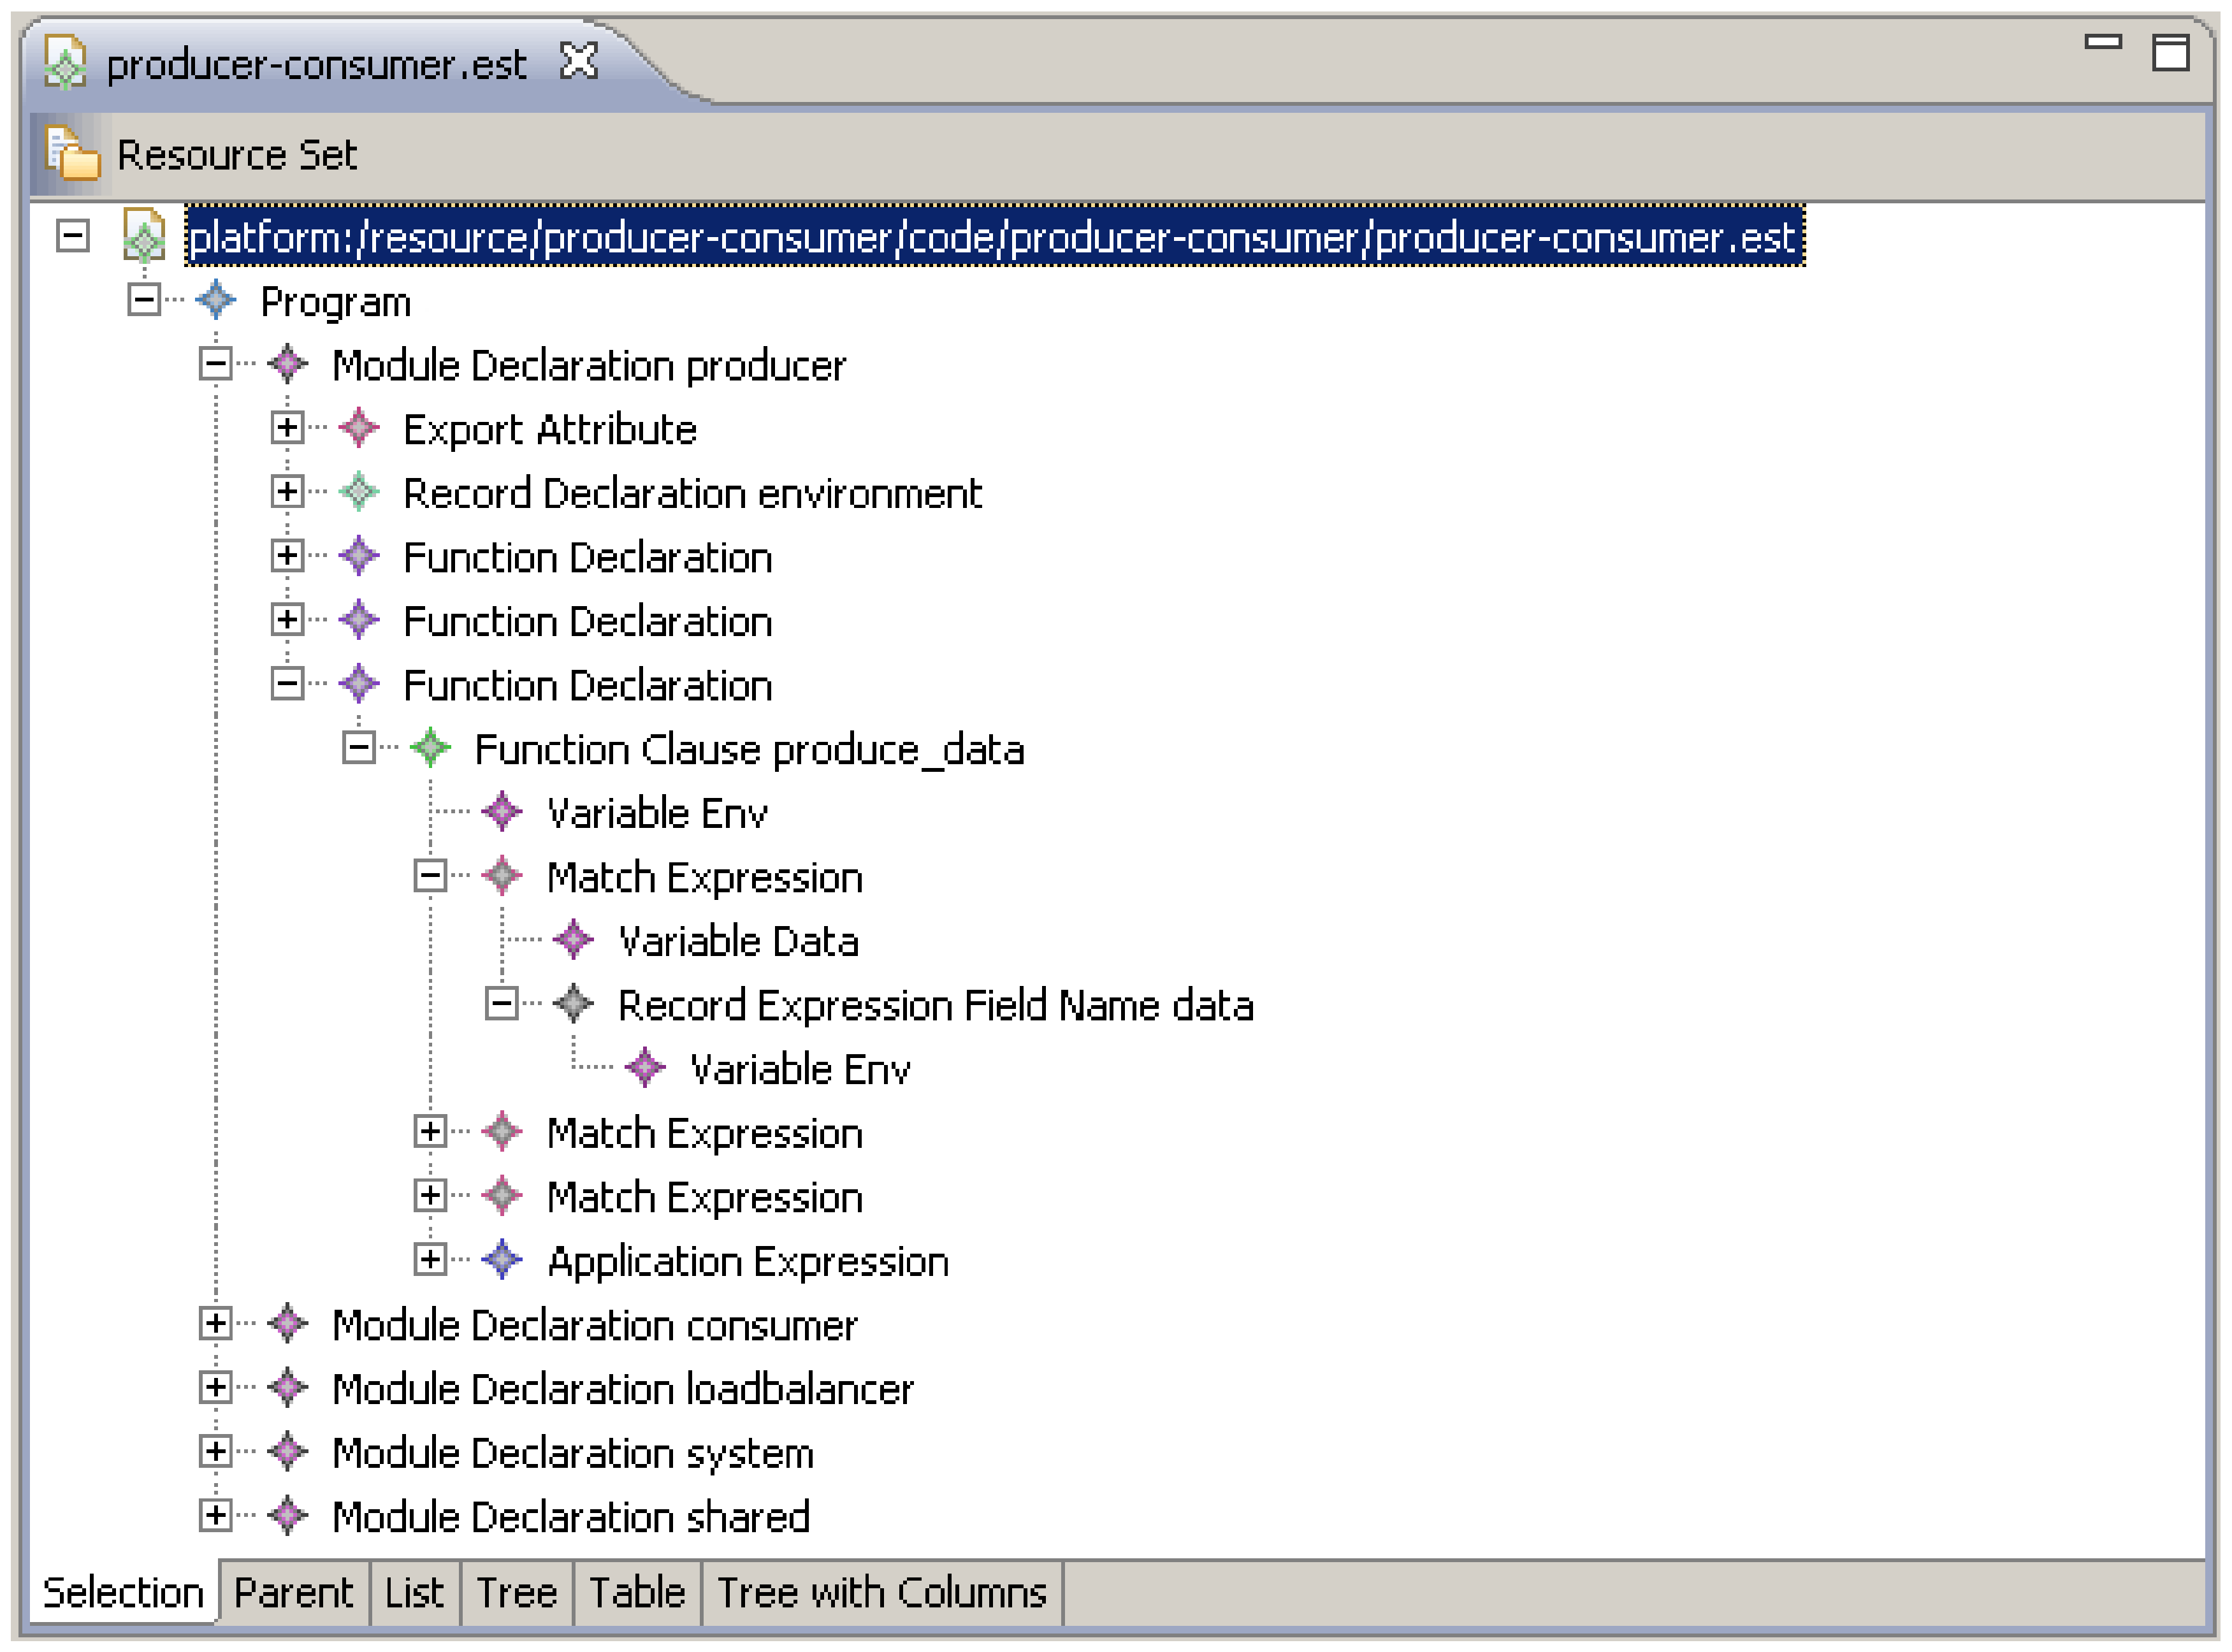
\includegraphics[scale=0.2]{techniques_and_tool/graphics/est.eps}
%\caption{The generated Erlang Syntax Tree (EST)}
%\label{fig:cgest}
%\end{figure}

\subsection{Implementation Details}
We have implemented the tool using the phases described in chapter~\ref{chap:translation}, i.e., CPN $\rightarrow$ decorated CPN $\rightarrow$ CFG $\rightarrow$ AST $\rightarrow$ EST $\rightarrow$ Erlang source code. All phases are completely independent in the implementation in the sense that a given phases takes an EMF model and returns a new EMF model. This showed to be very convenient in the development of the tool. Using the EMF framework it is easy to build, e.g., an example AST and use this model when implementing the AST $\rightarrow$ EST phase. Making the phases independent of each other also has the advantage that is it possible to substitute the Erlang dependent phases with, e.g., Java phases.
\section{Validating the Generated DYMO Code}
\label{sec:dymoexperiments}
In this section we give an impression of the generated code from the DYMO model, and explain the manual work that needs to be done in order to be able to execute the code. We also validate the generated Erlang code by using a simple network simulator to simulate the transmission of messages in a MANET. The implementation is executed, and the routing tables are inspected to verify that the connections were correctly established.

\subsection{Generating the Code and Implementing the Functions}

Generating the code from the DYMO model yields the modules shown in Table~\ref{table:gencodestat}. All these modules can be found in appendix \ref{appsec:dymocode_unmod}. We have listed lines of code (L.O.C.) for each module -- in total we generated 563 lines of code. Since we do not support automatic translation from CPN ML to Erlang, we had to manually implement various Erlang expressions and functions on the basis of the corresponding CPN ML code. These CPN ML expressions are carried along as comments in the generated code. The comments are placed where the expression should be used, thus the structure of the program is preserved. Implementing the functions (12 in total) in Erlang is an easy task, because of the similarity between Erlang and CPN ML. In appendix \ref{appsec:dymocode_mod} we show the modified modules. We spent approximately 12 person-hours modifying the generated code, but the time spent would be eliminated if we had an automatic translation from CPN ML to Erlang. 

\begin{table}
\vspace*{1em}
\begin{center}
\begin{tabular}{llllll}
    Module name  	& & L.O.C.	& & Functions to implement \\  \noalign{\smallskip}\hline\noalign{\smallskip}
	system.erl 		& & 20	& & 0 \\	
	buffer.erl 		& & 36  & & 0 \\
	shared.erl 		& & 16 	& & 0 \\
	initiator.erl 	& & 116	& & 1 [createRREQ] \\
	receiver.erl  	& & 116 & & 7 [isOwnMessage, isNewRoute, \dots] \\
	                                % isStale, isLoopPossible,isInferior, isSuperiorm, updateRouteEntry] \\
	processer.erl 	& & 111 & & 4 [isRREP, isRREQ, isTarget, \dots] \\
									%isRREP, isRREQ, isTarget, createRREP
	establishchecker.erl & & 126  & & 0 \\
	network.erl 	& & 22	& & 0 \\	
	   
	\noalign{\smallskip}\hline\noalign{\smallskip}
	Total & & 563 & & 12
	\\ \noalign{\smallskip}\hline\noalign{\smallskip}
\end{tabular}
\vspace*{1em}
\end{center}   
\caption{The Generated Modules from the DYMO Protocol}
\label{table:gencodestat}
\end{table} 

\begin{figure}[b!]
\begin{verbatim}
  rreq_target(Env) -> 
  Msg = Env#environment.message_for_processing,
  Ip = Env#environment.own_process_ip_address,
  routing_table ! {get, self()},
  receive 
    Rota -> 
      Rota
  end,
  seqnum ! {get, self()},
  receive 
    Seqnum -> 
      Seqnum
  end,
  NewEnv = Env#environment {},
  routing_table ! {set, Rota},
  seqnum ! {set, Seqnum},
  Id1 = 1,
  Receiver1 = list_to_atom("network_ID" ++
  integer_to_list(Id1) ++ "_dymo_to_network"),
  Receiver1 ! {send, %% createRREP(ip, msg, rota, seqNum)
  undefined},
  receive_incoming_message(NewEnv).
\end{verbatim}
\end{figure}

To give an impression of the task of manually implementing the CPN ML functions we take a look at some of the generated code. In Listing~\ref{fig:rreqtargetcode} we show the unmodified generated code for the \code{rreq\_target} function in the \code{processer} module. The \code{rreq\_target} function is called when a node discovers that it is the target of a route request message. A RREP message needs to be created in order to make a reply. In the CPN model the reply message is created by a CPN ML function. In line 20 of Listing~\ref{fig:rreqtargetcode} we see the CPN ML function \code{createRREP} as a commment. What needs to be done is to translate the CPN ML function \code{createRREP} to an equivalent Erlang function.

We have done this by replacing line 20 and 21 with the single line shown in Listing~\ref{fig:createRREPcall}.

\begin{figure}[h!]
\begin{verbatim}
Receiver1 ! {send, createRREP(Ip, Msg, Rota, SeqNum)},
\end{verbatim}
\end{figure}

The difference is that the comment character (\%) has been removed and the casing of the arguments to the function has been changed. Notice, that the function \code{createRREP} is given some arguments. These arguments has either been extracted from the environment or read from global variables. What is left to be done is implementing the function \code{createRREP}.

\begin{figure}[h!]
\begin{verbatim}
createRREP(Msg, Own_ip, Rota, SeqNum) ->
  Entry = util:get_entry(Msg#message.orig_addr, Rota),
  Next_hop_address =
             Entry#routing_table_entry.next_hop_address,
  #message {src = Own_ip, dest = Next_hop_address,
            target_addr = Msg#message.orig_addr, 
            orig_addr = Own_ip, orig_seqnum = SeqNum, 
            hop_limit = 5, dist = 1, msg_type = 'RREP'}.
\end{verbatim}
\end{figure}

The created Erlang function \code{createRREP} (shown in Listing~\ref{fig:createRREPfunction}) first extracts the entry of the originator of the request from the routing table. Then the next hop address is found in the entry. This information, along with information from the message and the sequence number, is used to create the reply message according to the DYMO specification.

\subsection{Setting-up a Network Simulation}
In order to execute more than one node running the generated DYMO implementation, we use the \emph{distributed Erlang system} which is a mechanism in Erlang allowing a number of Erlang systems to communicate over a network. It consists of a number of independent Erlang runtime systems. Each runtime system is called an \code{Erlang node}, and each node executes the same generated DYMO code. An advantage of using the distributed Erlang system is that each node has its own \emph{name space}, thus all the generated names of process instances does not have to be modified. For instance, in the \code{system} module all the registered names can remain unchanged.

The processes running the DYMO implementation on different Erlang nodes do not communicate directly with each other. Instead they communicate through a \emph{network simulator} process running on a separate Erlang node. The stub code for the network simulator was generated directly from the \code{network} process partition of the DYMO ProPCPN model (see bottom of Fig.~\ref{fig:systemmodule}). This means that the generated \code{initiator} and \code{processer} processes sends messages to the network by sending them to the buffer of the \code{network} process. Also, the \code{receiver} process is ready to receive messages from the network through its buffer. The network simulator process implements a simple MANET with a static topology where both unicast and multicast is supported. The topology is implemented by using an adjacency list representation. For each node there is a list specifying which nodes are in direct transmission range. When the destination address in a message is a unicast address it is passed directly to the node with the given address, and when a message contains a multicast address the message is passed to each node in the adjacency list of the sending node.

\subsection{Results of the Execution}
The generated DYMO code was then executed in the distributed environment. To monitor the behaviour of the program, each node prints its own routing table, which can then be inspected to verify that the expected routes were established. The first tests were done with topologies containing two and three nodes, and we found that routes were established as expected.

The generated DYMO code was then executed in the topology shown in Fig.~\ref{fig:mscrreq} with five nodes where node 1 is requesting a route to node 5. After the execution we inspected the routing tables of the nodes in the network. Node 1 had the following routing table:

\begin{center}
\begin{tabular}{|c|c|c|c|}
\hline
\multicolumn{4}{|c|}{\textbf{Routing table of node 1}} \\
\hline
\textit{Address} & \textit{SeqNum} & \textit{NextHopAddress} & \textit{Dist} \\
\hline
node 5 & 1 & node 2 & 2 \\
\hline
\end{tabular}
\end{center}

\noindent As we can see, node 1 has an entry for a route to node 5 through node 2 with a distance of 2. The routing table for node 2 was as follows:

\begin{center}
\begin{tabular}{|c|c|c|c|}
\hline
\multicolumn{4}{|c|}{\textbf{Routing table of node 2}} \\
\hline
\textit{Address} & \textit{SeqNum} & \textit{NextHopAddress} & \textit{Dist} \\
\hline
node 1 & 1 & node 1 & 1 \\
\hline
node 5 & 1 & node 5 & 1 \\
\hline
\end{tabular}
\end{center}

\noindent Node 2 has two entries for routes in its routing table, namely for node 1 and node 5. These entries show, that node 2 can send messages directly to both node 1 and node 5. This means that other nodes can send messages to node 1 and node 5 through node 2. Finally, the routing table on node 5:

\begin{center}
\begin{tabular}{|c|c|c|c|}
\hline
\multicolumn{4}{|c|}{\textbf{Routing table of node 5}} \\
\hline
\textit{Address} & \textit{SeqNum} & \textit{NextHopAddress} & \textit{Dist} \\
\hline
node 1 & 1 & node 2 & 2 \\
\hline
\end{tabular}
\end{center}

\noindent This routing table has a single entry for a route to node 1 through node 2 with a distance of 2. It can be seen that the route between node 1 and node 5 was correctly established in both directions. 

\begin{figure}
\centering
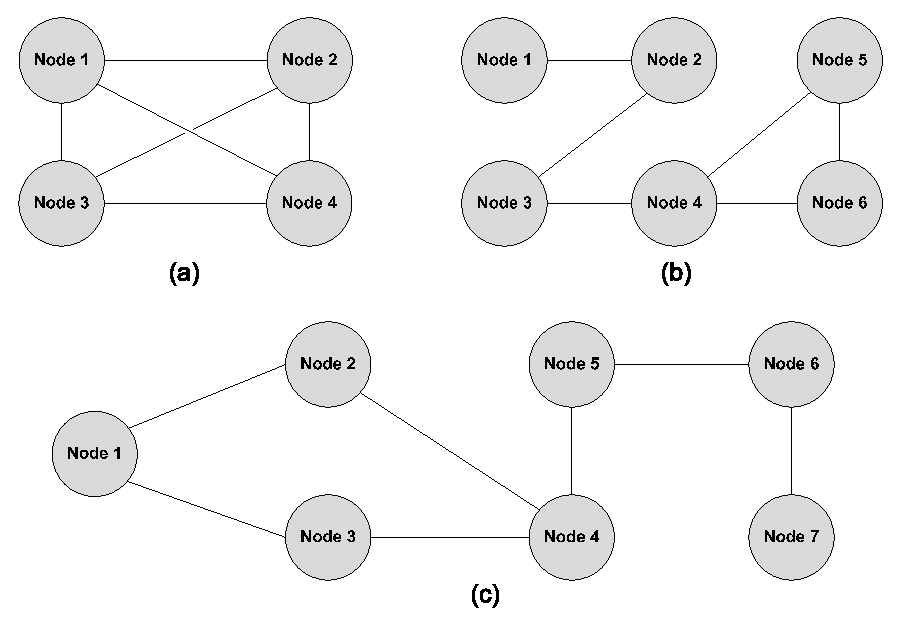
\includegraphics[scale=0.8]{dymo/graphics/topologies.eps}
\caption{Topologies to test the generated DYMO code}
\label{fig:topologies}
\end{figure}

To make sure that every part of the generated code at some point has been executed we have executed the generated DYMO code in the topologies shown in Fig.~\ref{fig:topologies}. In topology (a), node 1 makes a route request for node 4. This has the effect that all functions used to determine the usefulness of routing information is executed at least once. In topology (b), node 1 is requesting a route to node 6. This shows that the nodes are capable of establishing a route which consists of four hops. To further investigate the length of the routes we constructed topology (c), where node 1 is requesting a route to node 7. This test the part of the code that deals with the hop limit of a message. The shortest route between node 1 and node 7 has four intermediate nodes. When executing the protocol, where the messages contain a hop limit of four, the route could not be established. By increasing the hop limit to five the route was established through the four intermediate hops. Having all parts of the generated code executed with the expected outcome builds confidence in the correctness of the generated code.


\chapter{Code Generation from the ProPCPN DYMO Model}
\label{chap:dymo}
The producer-consumer system, we have focused on until now, is a small ProPCPN model created to illustrate the basic concepts. In this chapter we describe how code is generated from a ProPCPN model of the Dynamic MANET On-demand (DYMO) routing protocol, which is an advanced industrial-sized communication protocol. The DYMO protocol is introduced in section~\ref{sec:dymooverview}. In section~\ref{sec:dymomodel} we present a ProPCPN model of the DYMO protocol which contains more advanced modelling constructs than the producer-consumer ProPCPN model. In section~\ref{sec:dymoexperiments} we describe and validate the code generated from the DYMO model. 

\section{The DYMO Protocol}
\label{sec:dymooverview}
The Dynamic MANET On-demand routing protocol is a routing protocol for \emph{mobile ad-hoc networks} (MANETs). It is currently under development by the IETF MANET working group \cite{RefWorks:89}. The specification is an Internet-draft \cite{RefWorks:88}, and is expected to become a Request for Comments (RFC) document in the near future.

\subsection{Mobile Ad-hoc Networks}
A MANET \cite{RefWorks:90} is a network consisting of mobile nodes, e.g., laptops, or mobile phones. The network has no pre-existing communication infrastructure in contrast to, e.g., WLANs where the nodes communicate with each other through a base station. The nodes in a MANET must therefore communicate directly with one another, i.e., send messages to those nodes that are within physical transmission range. This means, that it is the power of the radio, and the physical position of the nodes, that determine the topology of the network. The topology of the network may change rapidly because of node mobility, and links between nodes might disappear and reappear frequently. A typical use of MANETs is during emergency search-and-rescue operations in remote areas where no pre-existing communication infrastructure exists. 

\newpage

In order to communicate with nodes outside a given nodes physical range a routing protocol is needed to perform multi-hop communication, i.e., nodes forward data packets on behalf of other nodes in the network. The topology of a small MANET with five nodes is shown in Fig.~\ref{fig:topology}. An edge between two nodes indicates that the nodes are within direct transmission range of each other, e.g., node 1 is able to send messages directly to node 2 and node 3. 

\begin{figure}
\centering
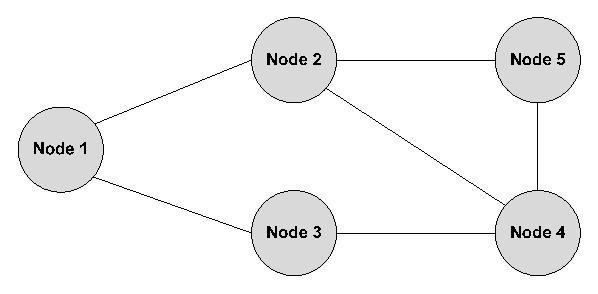
\includegraphics[scale=0.8]{dymo/graphics/topology_ex.eps}
\caption{Five node example topology}
\label{fig:topology}
\end{figure}

Routing protocols for MANETs are often categorised as being either \emph{proactive} or \emph{reactive}. The proactive routing protocols are constantly trying to keep an updated view of the network topology by maintaining a route to the other nodes in the network. The reactive routing protocols establish routes on demand, i.e., when routes are needed, and often do little maintenance on existing routes.

\subsection{The Operations of DYMO}
The DYMO routing protocol is a reactive protocol which establishes routes only when they are needed. The protocol has two main parts which are \emph{route discovery} and \emph{route maintenance}. Route maintenance is done by using active link monitoring and timeouts. If a node becomes aware that a route is broken it sends a \emph{Route Error} (RERR) message to the surrounding nodes, and thereby informs them that the route can no longer be used.

Route discovery is used to establish routes to other nodes in the network. An \emph{originator} node multicasts a \emph{Route Request} (RREQ) message which is sent hop-by-hop throughout the network to find a route to the \emph{target} node of the request. Each intermediate node records a route back to the originator node. When the target node receives the RREQ message it replies with a \emph{Route Reply} (RREP) message. This is unicasted back hop-by-hop towards the originator node using the routes recorded when the RREQ was sent. When the originator node receives the RREP message, the route has been established between the originator node and the target node in both directions.


\begin{figure}
\centering
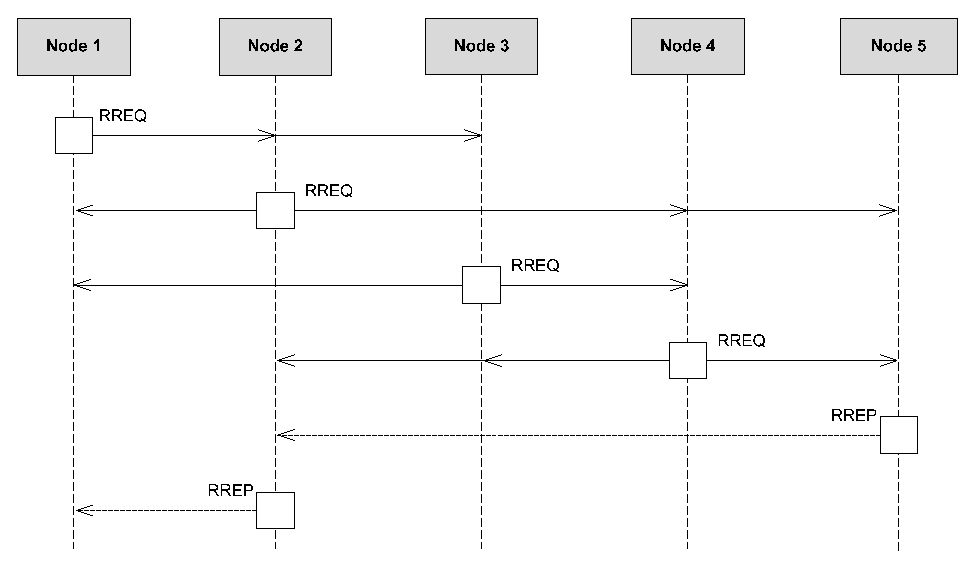
\includegraphics[width=\textwidth]{dymo/graphics/mscdymoex.eps}
\caption{Message sequence chart of a route request}
\label{fig:mscrreq}
\end{figure}

To get a better understanding of the protocol we present an example of how route discovery is performed in the small MANET shown in Fig.~\ref{fig:topology}. Fig.~\ref{fig:mscrreq} shows a message sequence chart (MSC) of one possible exchange of messages in the DYMO protocol when the originator node 1 is requesting a route to the target node 5. A solid arc represents multicast, and a dashed arc represents unicast. In the MSC, node 1 initiates the route request by multicasting a RREQ which is received by nodes 2 and 3. Node 2 and node 3 both records the route back to node 1 in their \emph{routing tables}, and then forwards the RREQ. Node 2 multicasts the RREQ message which is received by the nodes within transmission range, i.e., node 1, node 4, and node 5. Node 3 also multicasts the RREQ message which is received by node 1, and node 4. Node 1 discards the RREQs from node 2 and node 3 because it is the originator of the message. Node 4 first receives the RREQ from node 2 and records the route back to node 1. When node 4 receives the RREQ from node 3, it has already recorded a route to node 1 with the same length (number of hops) and the message is discarded.

Node 4 then multicasts the RREQ which is received by node 2, node 3, and node 5. The message is discarded by node 2 and node 3 since they already know of a shorter route to the originator node 1. Node 5 has received a RREQ from both node 2 and node 4, but since the RREQ from node 2 has a shorter route to node 1 this route is recorded in the routing table. Furthermore, node 5 is the target of the RREQ, and therefore replies with a RREP message with node 1 as the target. The RREP is unicasted back along the same route as the RREQ was sent which means that node 5 sends the RREP to node 2. When node 2 receives the RREP it already knows a route to node 1 (because of the RREQ) and unicasts the RREP to node 1. When node 1 receives the RREP a route is established between node 1 and node 5 in both directions.
\section{Modelling the DYMO Protocol}
\label{sec:dymomodel}

In this section we present the ProPCPN model of the DYMO protocol. The model is constructed on the basis of the DYMO CPN model presented in \cite{RefWorks:6}. The main difference between the model presented in this section, and the model in \cite{RefWorks:6}, is that the control flow of the protocol and access of variables is represented in the structure of the ProPCPN model which is characteristic for the ProPCPN models. The model presented in this section only captures the behaviour of the route discovery part of the protocol. To make the model more readable we present a hierarchical version of the model. Using a hierarchical ProPCPN model do not add expressive power since a hierarchical CPN model (and thus a PropCPN model) can always be transformed to an equivalent non-hierarchical CPN model with the same behaviour (p. 130, \cite{RefWorks:87}). A hierarchical CPN model is organised as a set of hierarchically related \emph{modules}. A module contains places and transitions, and can be seen as a component of the full CPN model.

\subsubsection{The System Module}

\begin{figure}[b!]
\centering
\includegraphics[width=\textwidth]{dymo/graphics/systemmodule.eps}
\caption{The \figitem{System} module of the ProPCPN DYMO model}
\label{fig:dymosystemmodule}
\end{figure}

Fig.~\ref{fig:dymosystemmodule} shows the prime (the root) module \figitem{System} of the ProPCPN DYMO model. The \figitem{System} module contains five \emph{substitution transitions} which are drawn as rectangular boxes with double lines. The substitution transitions are named \figitem{Establishchecker}, \figitem{Initiator}, \figitem{Network}, \figitem{Receiver}, and \figitem{Processer}. Each substitution transition is associated with a module which models the behaviour of the substitution transition. Tokens are exchanged between module using \emph{ports}. The ports constitutes the \emph{interface} of the module, i.e., a module can receive input via \emph{input ports}, and produce output via \emph{output ports}. In Fig.~\ref{fig:dymosystemmodule} all places are \emph{sockets}, i.e., places that are associated with an input or output port. The \figitem{System} module ties together the different parts of the protocol. The \figitem{Initiator} substitution transition creates new route requests. The \figitem{Establishchecker} substitution transition is responsible for notifying when a route has been established. The \figitem{Receiver} substitution transition judges the usefulness of the routing information found in received messages. The routing table is updated with the routing information if it is found useful. The messages that have not been discarded by the \figitem{Receiver} are send to the \figitem{Processer} that processes the messages depending on the message being a request or a reply. When the \figitem{Processer} has processed the message it can forward messages. The \figitem{Network} module is a simple reliable network. It forwards messages which is added to \figitem{DYMOToNetwork} and delivers it to the receiver by adding it to the place \figitem{NetworkToDYMO}.

\subsubsection{The Initiator Module}

\begin{figure}[b!]
\centering
\includegraphics[width=\textwidth]{dymo/graphics/initiatormodule.eps}
\caption{The \figitem{Initiator} module of the ProPCPN DYMO model}
\label{fig:initiatormodule}
\end{figure}

Next, we take a closer look at the \figitem{Initiator} module shown in Fig.~\ref{fig:initiatormodule}. As mentioned this module is responsible for creating route request which is performed by the transition \figitem{CreateRREQ}. To create a route request the transition needs information about its own IP address, the target IP address, and the sequence number to put into the message. The IP address of a node is stored locally at the local place \figitem{OwnIPAddress}. The sequence number and the target IP address, is also used by the \figitem{Processer}, and is therefore modelled as shared places. To avoid too many arcs, which would make the model less readable, we have created shared places using \emph{fusion sets}. Places in different modules belonging to the same fusion set can be seen as one compound place, i.e., they always share the same marking, and they have the same colour set and initial marking.

The transition \figitem{CreateRREQ} do not produce route requests if a route already has been esbablished (determined by the shared place \figitem{RouteEstablished}), the retries limit has been reached (determined by the local place \figitem{RREQ\_TRIES}), or the request has been cancelled (determined by the local place \figitem{Cancel}). When a request has been made it is added to the buffer place \figitem{DYMOToNetwork}. This place has the \emph{output port tag} attached to show that it is an output port. As we saw in the \figitem{System} module in Fig.~\ref{fig:dymosystemmodule}, this place is assigned to a socket place with the same name connected to the \figitem{Network} substitution transition.

The other two transitions in the module handle the cancelation of requests. \figitem{RREQ\_TRIESReached} is enabled when the maximum number of retries has been reached, and it sets the value of the local place \figitem{Cancel} to true. When \figitem{Cancel} is true \figitem{CancelRequest} is enabled which means that no further action should be taken with this request.

\subsubsection{The Processer Module}
\begin{figure}
\centering
\includegraphics[width=\textwidth]{dymo/graphics/processermodule.eps}
\caption{The \figitem{Processer} module of the ProPCPN DYMO model}
\label{fig:processermodule}
\end{figure}

Moving on to Fig.~\ref{fig:processermodule} we find the \figitem{Processer} module. The \figitem{Processer} receives messages from the \figitem{Receiver} on the buffer place \figitem{IncomingMessages}. When a message arrives, the transition \figitem{ReceiveIncomingMessage} becomes enabled, and when it occurs the message is added to the local place \figitem{MessageForProcessing} for further processing. The process token is then added to the process place \figitem{ProcessingMessage}, and the control flow either continues to the substitution transition \figitem{RREPprocesser} or to the substitution transition \figitem{RREQprocesser} (depending on the type of the message).

\subsubsection{The RREPprocesser Module}
\begin{figure}
\centering
\includegraphics[width=\textwidth]{dymo/graphics/rrepprocessermodule.eps}
\caption{The \figitem{RREP processer} module of the ProPCPN DYMO model}
\label{fig:rrepprocessermodule}
\end{figure}

The \figitem{RREPprocesser} module (shown in Fig.~\ref{fig:rrepprocessermodule}) processes incoming messages which has the type RREP, i.e., a route reply. The messages are added to the local place \figitem{MessageForProcessing}, and if the current node is the target, the transition \figitem{RREPTarget} is enabled. An occurrence of \figitem{RREPTarget} means that the route has been established, and by adding the IP address of the originator of the RREP to the buffer place \figitem{NewConnectionEstablished} the \figitem{Establishchecker} is notified. If the current node is not the target of the RREP the transition \figitem{RREPForward} can occur. The transition \figitem{RREPForward} creates a new RREP message with the use of the shared place \figitem{SeqNum}, the shared place \figitem{RoutingTable}, and the local place \figitem{OwnProcessIPAddress}. The newly created message is added to the buffer place \figitem{DYMOToNetwork} and can then be transmitted over the network.

\section{Validating the Generated DYMO Code}
\label{sec:dymoexperiments}
In this section we give an impression of the generated code from the DYMO model, and explain the manual work that needs to be done in order to be able to execute the code. We also validate the generated Erlang code by using a simple network simulator to simulate the transmission of messages in a MANET. The implementation is executed, and the routing tables are inspected to verify that the connections were correctly established.

\subsection{Generating the Code and Implementing the Functions}

Generating the code from the DYMO model yields the modules shown in Table~\ref{table:gencodestat}. All these modules can be found in appendix \ref{appsec:dymocode_unmod}. We have listed lines of code (L.O.C.) for each module -- in total we generated 563 lines of code. Since we do not support automatic translation from CPN ML to Erlang, we had to manually implement various Erlang expressions and functions on the basis of the corresponding CPN ML code. These CPN ML expressions are carried along as comments in the generated code. The comments are placed where the expression should be used, thus the structure of the program is preserved. Implementing the functions (12 in total) in Erlang is an easy task, because of the similarity between Erlang and CPN ML. In appendix \ref{appsec:dymocode_mod} we show the modified modules. We spent approximately 12 person-hours modifying the generated code, but the time spent would be eliminated if we had an automatic translation from CPN ML to Erlang. 

\begin{table}
\vspace*{1em}
\begin{center}
\begin{tabular}{llllll}
    Module name  	& & L.O.C.	& & Functions to implement \\  \noalign{\smallskip}\hline\noalign{\smallskip}
	system.erl 		& & 20	& & 0 \\	
	buffer.erl 		& & 36  & & 0 \\
	shared.erl 		& & 16 	& & 0 \\
	initiator.erl 	& & 116	& & 1 [createRREQ] \\
	receiver.erl  	& & 116 & & 7 [isOwnMessage, isNewRoute, \dots] \\
	                                % isStale, isLoopPossible,isInferior, isSuperiorm, updateRouteEntry] \\
	processer.erl 	& & 111 & & 4 [isRREP, isRREQ, isTarget, \dots] \\
									%isRREP, isRREQ, isTarget, createRREP
	establishchecker.erl & & 126  & & 0 \\
	network.erl 	& & 22	& & 0 \\	
	   
	\noalign{\smallskip}\hline\noalign{\smallskip}
	Total & & 563 & & 12
	\\ \noalign{\smallskip}\hline\noalign{\smallskip}
\end{tabular}
\vspace*{1em}
\end{center}   
\caption{The Generated Modules from the DYMO Protocol}
\label{table:gencodestat}
\end{table} 

\begin{figure}[b!]
\begin{verbatim}
  rreq_target(Env) -> 
  Msg = Env#environment.message_for_processing,
  Ip = Env#environment.own_process_ip_address,
  routing_table ! {get, self()},
  receive 
    Rota -> 
      Rota
  end,
  seqnum ! {get, self()},
  receive 
    Seqnum -> 
      Seqnum
  end,
  NewEnv = Env#environment {},
  routing_table ! {set, Rota},
  seqnum ! {set, Seqnum},
  Id1 = 1,
  Receiver1 = list_to_atom("network_ID" ++
  integer_to_list(Id1) ++ "_dymo_to_network"),
  Receiver1 ! {send, %% createRREP(ip, msg, rota, seqNum)
  undefined},
  receive_incoming_message(NewEnv).
\end{verbatim}
\end{figure}

To give an impression of the task of manually implementing the CPN ML functions we take a look at some of the generated code. In Listing~\ref{fig:rreqtargetcode} we show the unmodified generated code for the \code{rreq\_target} function in the \code{processer} module. The \code{rreq\_target} function is called when a node discovers that it is the target of a route request message. A RREP message needs to be created in order to make a reply. In the CPN model the reply message is created by a CPN ML function. In line 20 of Listing~\ref{fig:rreqtargetcode} we see the CPN ML function \code{createRREP} as a commment. What needs to be done is to translate the CPN ML function \code{createRREP} to an equivalent Erlang function.

We have done this by replacing line 20 and 21 with the single line shown in Listing~\ref{fig:createRREPcall}.

\begin{figure}[h!]
\begin{verbatim}
Receiver1 ! {send, createRREP(Ip, Msg, Rota, SeqNum)},
\end{verbatim}
\end{figure}

The difference is that the comment character (\%) has been removed and the casing of the arguments to the function has been changed. Notice, that the function \code{createRREP} is given some arguments. These arguments has either been extracted from the environment or read from global variables. What is left to be done is implementing the function \code{createRREP}.

\begin{figure}[h!]
\begin{verbatim}
createRREP(Msg, Own_ip, Rota, SeqNum) ->
  Entry = util:get_entry(Msg#message.orig_addr, Rota),
  Next_hop_address =
             Entry#routing_table_entry.next_hop_address,
  #message {src = Own_ip, dest = Next_hop_address,
            target_addr = Msg#message.orig_addr, 
            orig_addr = Own_ip, orig_seqnum = SeqNum, 
            hop_limit = 5, dist = 1, msg_type = 'RREP'}.
\end{verbatim}
\end{figure}

The created Erlang function \code{createRREP} (shown in Listing~\ref{fig:createRREPfunction}) first extracts the entry of the originator of the request from the routing table. Then the next hop address is found in the entry. This information, along with information from the message and the sequence number, is used to create the reply message according to the DYMO specification.

\subsection{Setting-up a Network Simulation}
In order to execute more than one node running the generated DYMO implementation, we use the \emph{distributed Erlang system} which is a mechanism in Erlang allowing a number of Erlang systems to communicate over a network. It consists of a number of independent Erlang runtime systems. Each runtime system is called an \code{Erlang node}, and each node executes the same generated DYMO code. An advantage of using the distributed Erlang system is that each node has its own \emph{name space}, thus all the generated names of process instances does not have to be modified. For instance, in the \code{system} module all the registered names can remain unchanged.

The processes running the DYMO implementation on different Erlang nodes do not communicate directly with each other. Instead they communicate through a \emph{network simulator} process running on a separate Erlang node. The stub code for the network simulator was generated directly from the \code{network} process partition of the DYMO ProPCPN model (see bottom of Fig.~\ref{fig:systemmodule}). This means that the generated \code{initiator} and \code{processer} processes sends messages to the network by sending them to the buffer of the \code{network} process. Also, the \code{receiver} process is ready to receive messages from the network through its buffer. The network simulator process implements a simple MANET with a static topology where both unicast and multicast is supported. The topology is implemented by using an adjacency list representation. For each node there is a list specifying which nodes are in direct transmission range. When the destination address in a message is a unicast address it is passed directly to the node with the given address, and when a message contains a multicast address the message is passed to each node in the adjacency list of the sending node.

\subsection{Results of the Execution}
The generated DYMO code was then executed in the distributed environment. To monitor the behaviour of the program, each node prints its own routing table, which can then be inspected to verify that the expected routes were established. The first tests were done with topologies containing two and three nodes, and we found that routes were established as expected.

The generated DYMO code was then executed in the topology shown in Fig.~\ref{fig:mscrreq} with five nodes where node 1 is requesting a route to node 5. After the execution we inspected the routing tables of the nodes in the network. Node 1 had the following routing table:

\begin{center}
\begin{tabular}{|c|c|c|c|}
\hline
\multicolumn{4}{|c|}{\textbf{Routing table of node 1}} \\
\hline
\textit{Address} & \textit{SeqNum} & \textit{NextHopAddress} & \textit{Dist} \\
\hline
node 5 & 1 & node 2 & 2 \\
\hline
\end{tabular}
\end{center}

\noindent As we can see, node 1 has an entry for a route to node 5 through node 2 with a distance of 2. The routing table for node 2 was as follows:

\begin{center}
\begin{tabular}{|c|c|c|c|}
\hline
\multicolumn{4}{|c|}{\textbf{Routing table of node 2}} \\
\hline
\textit{Address} & \textit{SeqNum} & \textit{NextHopAddress} & \textit{Dist} \\
\hline
node 1 & 1 & node 1 & 1 \\
\hline
node 5 & 1 & node 5 & 1 \\
\hline
\end{tabular}
\end{center}

\noindent Node 2 has two entries for routes in its routing table, namely for node 1 and node 5. These entries show, that node 2 can send messages directly to both node 1 and node 5. This means that other nodes can send messages to node 1 and node 5 through node 2. Finally, the routing table on node 5:

\begin{center}
\begin{tabular}{|c|c|c|c|}
\hline
\multicolumn{4}{|c|}{\textbf{Routing table of node 5}} \\
\hline
\textit{Address} & \textit{SeqNum} & \textit{NextHopAddress} & \textit{Dist} \\
\hline
node 1 & 1 & node 2 & 2 \\
\hline
\end{tabular}
\end{center}

\noindent This routing table has a single entry for a route to node 1 through node 2 with a distance of 2. It can be seen that the route between node 1 and node 5 was correctly established in both directions. 

\begin{figure}
\centering
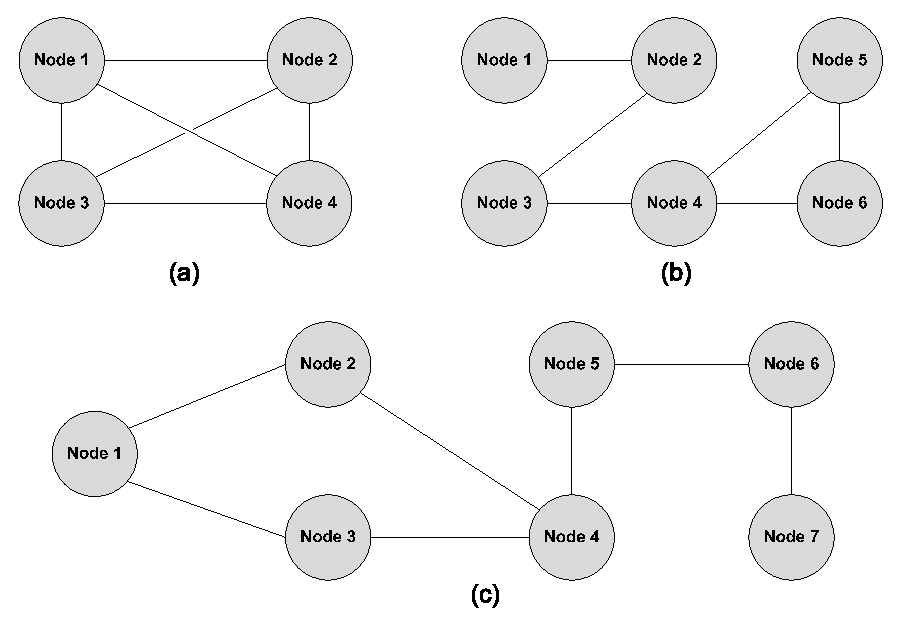
\includegraphics[scale=0.8]{dymo/graphics/topologies.eps}
\caption{Topologies to test the generated DYMO code}
\label{fig:topologies}
\end{figure}

To make sure that every part of the generated code at some point has been executed we have executed the generated DYMO code in the topologies shown in Fig.~\ref{fig:topologies}. In topology (a), node 1 makes a route request for node 4. This has the effect that all functions used to determine the usefulness of routing information is executed at least once. In topology (b), node 1 is requesting a route to node 6. This shows that the nodes are capable of establishing a route which consists of four hops. To further investigate the length of the routes we constructed topology (c), where node 1 is requesting a route to node 7. This test the part of the code that deals with the hop limit of a message. The shortest route between node 1 and node 7 has four intermediate nodes. When executing the protocol, where the messages contain a hop limit of four, the route could not be established. By increasing the hop limit to five the route was established through the four intermediate hops. Having all parts of the generated code executed with the expected outcome builds confidence in the correctness of the generated code.



\chapter{Conclusion and Future Work}
\label{chap:confutwo}

In this thesis we showed how to automatically generate code from a CPN model to a target programming language using a structural code generation approach. We described the translation from ProPCPN to the Erlang programming language, and as a proof of concept we implemented a tool that, given a ProPCPN model, generates Erlang code. The generated code from a simple producer-consumer ProPCPN model was validated, and we found that the behaviour of the executions were equivalent to the behaviour of the CPN model. We investigated the expressive power of the constructed net class by modelling the industrial-sized routing protocol DYMO in ProPCPN, and validations indicated that the generated code was correct. In the following we summaries and conclude on the presented topics in this thesis.

\section{Approaches to Code Generation}
%discussion
% summary
Research done in related work shows that the chosen approach to automatic code generation from Petri nets has a large impact on the properties of the final code. Based on related work, we categorised automatic code generation from Petri nets into the four categories: decentralised, state space-, simulation- and structural-based. The state space based approach only works on small models because of the state explosion problem, and the decentralised approach would result in an enormous number of process instances for large models. We therefore decided to focus on the simulation-based and structural-based approach.

% simulation-based pro-cons
The main idea behind the simulation-based approach is to have a scheduler which, on the basis of the state of the environment, determines the control flow of the program. The process of determining which state to proceed to corresponds to finding enabled transitions in the CPN model. This resemblance to a CPN simulator makes it easier to capture the behaviour of the model in the program. Another advantage is that this approach does not restrict the net class that can be generated code from. The disadvantage of this approach is that the generated code tends to be in an unnatural programming style. This makes the code hard to modify or extend which may be required to adopt it into the environment in which it will be embedded. This approach also has the disadvantage that it can lead to inefficient code because the scheduler is called in between each state change which is time-consuming, and consequently can put a lot of overhead on the system.

% structural-based pro-cons
The code generated in the structural-based approach contains no central scheduler to control the flow of the program. The main idea is to recognise structures and regular patterns in the model, and have the control flow distributed across the program as jumps. Because of this, the structural-based approach produces more readable code than the simulation-based approach, since it looks more like it was written by a human programmer. The generated code would also often be more efficient, because the control flow is not controlled by a central component. The disadvantage of this approach is the restriction on the class of nets that code can be generated from. This is because general Petri nets provide much more opportunities of constructing different control flow structures than common programming languages.

% conclusion
We found that the structural-based approach was the most advantageous based on the discussion of the simulation-based and structural-based approaches. Generating readable code is very important to minimise the risk of introducing errors while extending and modifying the code. Furthermore, the simulation-based approach would be very similar to a CPN simulator, and they already exist, e.g., the simulator found in CPN Tools.

\section{Defining the ProPCPN Class}
In order to generate code in a structural-based manner we made a formal definition of a subclass of CPNs called Process-Partitioned Coloured Petri Nets (ProPCPNs). A ProPCPN is restricted in such a way that it is possible to recognise structures that can be translated into common programming language constructs. The main property of the class is that the CPN model can be partitioned into separate processes which run independently of each other. The control flow of a process is made explicit through the use of process places in the model. The control of a process can either flow unconditionally to another point, or conditionally to many points. It is possible to store data locally within a process instance using local places, and globally between process instances using shared places. A process instance can also send data to another process instance using buffer places. ProPCPN allow general CPN ML expressions, thus the expressive power of arc expressions and guard expressions are as strong as in CPN. 
   
\section{Generating Code from ProPCPN Models}
We created a technique for translating from ProPCPN models to a target language. The translation is divided into a number of phases, where the first three phases are independent of the target language. 

\subsection{Phase 1-3: Generating an AST}
The first phase is to decorate the ProPCPN model with process partitions, and assign types to places, transitions, and arcs. This is done in order to ease phase two, in which the decorated ProPCPN model is translated into a control flow graph (CFG). A CFG is constructed for each process partition of the ProPCPN model, and together they constitute the program. The translation in this phase consists of extracting the control flow from the model and making it explicit in the CFG, where it is represented as edges between blocks of statements. The phase also identifies program constructs, e.g., variables and synchronisation points, and translates them into statements. 

In phase three, the CFG is translated into an abstract syntax tree (AST) for a simple language that contains common program constructs. We have designed the language such that it can be translated into any common type of programming language. This phase translates the control flow given in the structure of the CFG into a tree consisting of nodes representing programming constructs. The statements in the blocks of the CFG are parsed and translated into subtrees in order to make the structure of statements explicit in the AST.

\subsection{Phase 3-5: Generating Erlang Source Code}
Until now, the phases of the translation have been independent of the target language. Phase four consists of translating the AST into a syntax tree for a specific programming language. We have chosen Erlang as the target programming language, thus we translate the AST into an Erlang program represented as an Erlang syntax tree (EST). The control flow, represented by goto statements in the AST, is translated into function calls, and the reading/writing of variables are translated into accessing/updating an environment record which is passed around with the function calls. Message passing between processes is native in Erlang which means that sending and receiving messages can be translated into native program constructs. 

The last phase prints the EST by traversing the tree and printing each node according the Erlang grammar. This produces the final Erlang source code which is the product of the translation. 

\section{Implementing the Translation}

% Technologies/TOOL: summary
As a proof of concept we have implemented the translation from ProPCPN models to Erlang code as an Eclipse plug-in for the ASAP tool. Through the use of wizards the user can import a CPN model into the workspace, and then generate Erlang code from that model. The user is also able to inspect the phases in the translation. Through the wizard the user can choose to have the CFG, AST, or EST written in files which can then be presented visually as tree structures. The implementation shows that the translation is indeed feasible in practise, and we found that extending the implementation with new features seemed fairly easy.  

% Evaluation: summary
To validate the generated Erlang code of the producer-consumer system, we compared it to manually translated code from the model. The generated code is very similar to code handwritten in the manually translated code. The code was also validated by executing it, and the behaviour of the program was documented in a message sequence chart. The results of the executions of the generated code showed that the messages being passed between the processes were as expected. The execution of the program was also compared with a simulation of the same scenario in the ProPCPN model, and we found the behaviour to be equivalent. This builds confidence in the behaviour of the ProPCPN model being preserved in the generated Erlang program.

\section{DYMO -- A Large ProPCPN Model}
%DYMO
% summary
To show the expressive power of the net class, and that the translation works for larger and more advanced models, we built a ProPCPN model of the DYMO routing protocol. The DYMO protocol is an advanced industrial-size communication protocol that allows multi-hop communication in MANETs. The DYMO model captures the behaviour of the route discovery part of the DYMO protocol. It consists of eight modules containing a total of 49 places and 18 transitions.

Erlang code was generated from the ProPCPN DYMO model and the Erlang functions and expressions where implemented which took approximately 12 person-hours of work. To validate the generated code we built a test environment in which the code could be executed. A network simulator made it possible to run the generated code for the protocol on a number of nodes. A scenario could then be executed and afterwards the state of the protocol could be inspected to verify that routes had been established as expected. The DYMO model showed that it is possible to construct a model of an advanced industrial-size communication protocol using the ProPCPN net class. It also showed that the translation is able to cope with more advanced control flow issues, e.g., control flow branches.

\section{Perspectives in Code Generation}
The work in this thesis shows that it is possible, in an automatic way, to generate program code from a ProPCPN model. The user can create a model, then verify importing properties of the model, and finally generate code with the same behaviour and properties as the model.

With the automatic code generation, the task of manually implementing the system is eliminated. This task is often error-prone and time-consuming, and therefore very costly. We created a net class and showed that the translation from this class is feasible. Finally, we showed that it is in fact possible to implement the translation technique, and that the generated code has the same properties and behaviour as the model. We believe that this is a great assistance in the development of programs without errors.

\section{Future Work}
\label{futurework}

Having more time to our disposal, there are a number of aspects about automatic code generation from CP-nets that would be interesting to investigate further.

\subsection{Extending the Class of ProPCP-nets}
The class of ProPCP-nets described has enough expressive power to model industrial-sized communication protocols, as we have shown with the DYMO ProPCPN model. However, we do have a restriction that tends to increase the size of the models. According to (7) in definition~\ref{def:propcpn} in section~\ref{sec:netclassformal}, it is not allowed to have variables in a transition guard that appear on an input arc from a buffer place or a shared place. Removing this restriction from the class of ProPCP-nets would reduce the size of the DYMO model. It would also complicate the translation from AST to EST though, because a guard in the current definition cannot change value once evaluated. Allowing, e.g., variables on input arcs from shared places in the guard expressions have the consequence that a guard can change value after being evaluated. This is because another process instance may change the value of the shared place after the guard has been evaluated. Therefore, a locking mechanism would have to be implemented in the generated code in order to ensure that the value of the corresponding global variable do not change before the jump has been made and the function has been executed. Without the locking mechanism, a conditional jump could be made based on one value and when the target function of the jump was evaluated the value had changed. This would mean that the generated program could have executions that were not possible in the CPN model it was generated from. 

\subsection{Formally Verifying the Translation}
In this thesis we have described and implemented a translation from ProPCPN models to Erlang code. We have validated the result of the translation by executing the generated code and monitoring the behaviour. The behaviour was compared to simulations in the CPN model. As a subject for future work it would be interesting to make a more formal verification of the steps in the translation. This should be done in order to have a proof that each step preserves the behaviour of the CPN model. A proof that the translation is correct does not necessarily mean that an implementation of the translation generates correct code since the implementation might be incorrect. Therefore, it would also be interesting to develop a method to more formally verify that the concrete generated code has the same behaviour as the CPN model it was generated from.

\subsection{Enhancing the Code Generation Tool}
In this thesis we have used the implemented tool as a proof of concept, but there is still some work to be done in order to enhance the usefulness of the tool. A hierarchical CPN model is often more readable than the equivalent flat model. Hierarchical models do not have more expressive power, since a hierarchical CPN model can always be flattened as mentioned in section \ref{sec:dymomodel}. Even though hierarchical models do not have more expressive power, it would be convenient if the tool supported hierarchical ProPCPN models, and automatically flattened them according to the steps in (p. 130, \cite{RefWorks:87}).

Expressions on arcs and in guards in a ProPCPN model are written in CPN ML. Our tool does not support automatic translation of these expressions, but having such an automatic translation would eliminate the need for manually modifying the generated code. It would also weed out some errors that might be introduced in the manual translation. Having the CPN ML and Erlang expressions in a parsed representation in the AST and EST would also allow for some optimisations. 

\subsection{Create a ProPCPN Editor Tool}
In this project we have used CPN Tools to create ProPCPN models. CPN Tools ensures that only valid CPN models can be created, e.g., that the initial marking of a place evaluates to a multi-set belonging to the colour set of that place. Having a ProPCPN editor has the following advantages: 

\begin{itemize}
\item The user is immediately prompted if trying to create something that is not allowed according to the ProPCPN definition, e.g., having an illegal colour set on a process place.
\item The ProPCPN models we have presented in this thesis are painted to better visually distinguish between the different place types. In a ProPCPN editor one could, e.g., have a toolbox containing the possibility of creating a local place which would automatically be painted green.  
\item The ProPCPN model created in the editor can then be given to the code generation tool. The tool does not need to check if the model is a ProPCPN model because the editor only outputs valid ProPCPN models
\item Most of the decoration in the first phase of the translation described in section \ref{sec:cpntodcpn} would be eliminated by having the user explicitly specifying the type of places.
\end{itemize}

The editor could be made, e.g., as an extension of CPN Tools, or using the Eclipse framework as we did with our implementation of the translation from ProPCPN to the Erlang programming language.


%\clearpage

\bibliographystyle{plain}
%\renewcommand{\bibname}{References}
\bibliography{literature}
\addcontentsline{toc}{chapter}{Bibliography}


\appendix
%\addappheadtotoc
\chapter{The Content of the Enclosed CD-ROM}
\label{appsec:cd}

On the enclosed CD-ROM we have included the implementation of the translation described in section \ref{sec:owntool}. The program can be executed by running \code{Code\_generation\_ASAP.exe} in the \code{TOOL} directory. We do not support hierarchical models in the current version, thus the model to generate code from has to be a flat ProPCPN model. The model can be created in CPN Tools but it is the creator of the model responsibility to check that it is in fact a ProPCPN model. Example ProPCPN models can be found on the cd (see below).

Otherwise, the following can be found on the cd:

\begin{enumerate}
  \item A directory named \textbf{Models} containing: the producer-consumer ProPCPN model, the hierarchical DYMO ProPCPN model, the flat DYMO ProPCPN model, and the DYMO CPN model we created in an earlier project. 
  \item A directory named \textbf{Report} containing PDF version of this report.
  \item A directory named \textbf{Generated code} containing the code generated from the producer-consumer ProPCPN mode and the DYMO ProPCPN model.   

\end{enumerate}

\noindent The same content can be found by visiting: \newline \url{http://www.daimi.au.dk/~keblov/thesis/}.

\chapter{The Full AST EBNF}
\label{app:astebnffull}

\footnotesize
\begin{verbatim}
                   <Program> ::= *<Process> *<GlobalVariableDeclaration>
 <GlobalVariableDeclaration> ::= <Name> <InitialExpression>
                   <Process> ::= <Name> *<Block> 
                                 *<ProcessVariableDeclaration>
                                 <EntryBlock>
                      <Name> ::= string
<ProcessVariableDeclaration> ::= <Name> <InitialExpression>
         <InitialExpression> ::= <Expression>
                     <Block> ::= <Name> <Statements>
                <EntryBlock> ::= <Block>
                
                <Statements> ::= *<Statement> |
                                 <Statements> <UnconditionalGotoStatement>
                 <Statement> ::= <LocalVariableDeclaration> |
                                 <ReadStatement> |
                                 <GlobalVariableReadStatement> |
                                 <ReceiveStatement>  |
                                 <WriteStatement> | <SendStatement> |
                                 <GlobalVariableWriteStatement> |
                                 <ConditionalGotoStatement>
             <ReadStatement> ::= <LocalVariableExpression>
                                 <ProcessVariableExpression>
            <WriteStatement> ::= <ProcessVariableExpression> <Expression>
             <SendStatement> ::= <Expression> <ProcessIDString>
          <ReceiveStatement> ::= <LocalVariableExpression>
  <LocalVariableDeclaration> ::= <Name>
  <ConditionalGotoStatement> ::= <Block> <Expression>
<UnconditionalGotoStatement> ::= <Block>
           <ProcessIDString> ::= string
           
                <Expression> ::= <BinaryOperatorExpression> |
                                 <LocalVariableExpression> |
                                 <GlobalVariableExpression> |
                                 <ProcessVariableExpression> |
                                 <UnknownExpression> |
                                 <IntegerConstantExpression> |
                                 <StringExpression> |
                                 <Undefined>
   <LocalVariableExpression> ::= <LocalVariableDeclString>
 <ProcessVariableExpression> ::= <ProcessVariableDeclString>
  <BinaryOperatorExpression> ::= <Expression> <Operator> <Expression>
 <IntegerConstantExpression> ::= integer
         <UnknownExpression> ::= string
                 <Undefined> ::= ""
                  <Operator> ::= + | - | * | /
   <LocalVariableDeclString> ::= string
 <ProcessVariableDeclString> ::= string
\end{verbatim}
\normalsize


\chapter{The Full EST EBNF}
\label{app:estebnffull}

\footnotesize
\begin{verbatim}
<Program>              ::= *<ModuleDecl>
<ModuleDecl>           ::= <ModuleName> *<HeaderForm> <ProgramForm> 
<ModuleName>           ::= string
<HeaderForm>           ::= <ExportAttribute> | 
                           <RecordDecl>
<ProgramForm>          ::= <FunctionDecl> |
                           *<ProgramForm> <FunctionDecl> |
                           *<ProgramForm> <RecordDecl> 
<ExportAttribute>      ::= *<FunctionName>
<RecordDecl>           ::= <RecordType> *<RecordFieldDecl>
<FunctionDecl>         ::= *<FunctionClause>  
<FunctionName>         ::= <FunctionSymbol> <arity>
<FunctionSymbol>       ::= string
<RecordType>           ::= string
<RecordFieldDecl>      ::= <RecordFieldName> ?<Expression>
<arity>                ::= int
<FunctionClause>       ::= <FunctionSymbol> ?<Pattern> *<Expression>
<RecordFieldName>      ::= string

<Pattern>              ::= <AtomicLiteral> |
                           <Variable> |
                           <TuplePattern> |
                           <RecordPattern> |
                           <ListPattern>
<AtomicLiteral>        ::= string
<Variable>             ::= string
<TuplePattern>         ::= *<Pattern>
<RecordPattern>        ::= <RecordType> <RecordFieldPattern>
<RecordType>           ::= string
<RecordFieldPattern>   ::= <RecordFieldName> <Pattern>
<RecordFieldName>      :: string
<ListPattern>          ::= *<Pattern>

<Expression>           ::= <ApplicationExp> |
                           <AtomicLiteral> |
                           <BinaryOperatorExp> |
                           <IfExp> |
                           <ListSkeleton> |
                           <MatchExp> |
                           <ParenthesizedExp> |
                           <ReceiveExp> |
                           <RecordExp> |
                           <SendExp> |
                           <TupleSkeleton> |
                           <Variable> 

<ApplicationExp>       ::= <Expression> *<Expression>
<BinaryOperatorExp>    ::= <Expression> <Operator> <Expression>
<Operator>             ::= string
<IfExp>                ::= *<IfClause>
<IfClause>             ::= *<Expression> *<Expression>
<ListSkeleton>         ::= *<Expression>
<MatchExp>             ::= <Pattern> <Expression>
<ParenthesizedExp>     ::= <Expression>
<ReceiveExp>           ::= *<CrClause>
<CrClause>             ::= <Pattern> *<Expression>
<RecordExp>            ::= ?<Expression> <RecordType> <RecordFieldNameExp> |
                           ?<Expression> <RecordType> <RecordUpdateTupleExp>
<RecordFieldNameExp>   ::= <RecordFieldName> 
<RecordUpdateTupleExp> ::= *<RecordFieldUpdate>
<RecordFieldUpdate>    ::= <RecordFieldName> <Expression>
<SendExp>              ::= <Expression> <Expression>
<TupleSkeleton>        ::= *<Expression>
\end{verbatim}
\normalsize

\chapter{Erlang Grammar}
\label{app:fullerlanggrammar}

This is the subset of Erlang we need to generate Erlang source code.


\footnotesize
\begin{verbatim}
ModuleDeclaration :
   ModuleAttribute HeaderForm* ProgramForms*

ModuleAttribute: 
   - module ( ModuleName ) FullStop 

ModuleName: 
   AtomLiteral

HeaderForm: 
   ExportAttribute |
   RecordDeclaration 

ExportAttribute: 
 - export ( FunctionNameList ) FullStop 

FunctionNameList : 
   [ FunctionNames? ]

FunctionNames : 
   FunctionName |
   FunctionNames , FunctionName 

FunctionName: 
   FunctionSymbol / Arity 

FunctionSymbol : 
   AtomLiteral 

Arity : 
   IntegerLiteral 

ProgramForms : 
   FunctionDeclaration |
   ProgramForms FunctionDeclaration |
   ProgramForms RecordDeclaration 

FunctionDeclaration: 
   FunctionClauses FullStop 

FunctionClauses : 
   FunctionClause |
   FunctionClauses ; FunctionClause 

FunctionClause : 
   FunctionSymbol FunClause 

RecordDeclaration : 
�   - record ( RecordType , RecordDeclTuple ) FullStop 

RecordDeclTuple: 
   { RecordFieldDecls? }
   
RecordFieldDecls : 
   RecordFieldDecl |
   RecordFieldDecls , RecordFieldDecl 

RecordFieldDecl : 
   RecordFieldName RecordFieldValue?

Pattern: 
   AtomicLiteral |
   Variable |
   TuplePattern |
   RecordPattern 

TuplePattern : 
   { Patterns? }
   
ListPattern :
   [] |
   [ Patterns ListPatternTail? ]
   
ListPatternTail : 
   | Pattern
   
Patterns : 
   Pattern |
   Patterns , Pattern 

RecordPattern : 
   # RecordType RecordPatternTuple 

RecordType : 
   AtomLiteral 

RecordPatternTuple: 
   { RecordFieldPatterns? }
   
RecordFieldPatterns : 
   RecordFieldPattern |
   RecordFieldPatterns , RecordFieldPattern 

RecordFieldPattern : 
   RecordFieldName = Pattern 

RecordFieldName: 
   AtomLiteral 

Exprs :
   Expr |
   Exprs , Expr

Expr :
   MatchExpr

MatchExpr : 
   Pattern = MatchExpr |
   SendExpr 

SendExpr : 
   CompareExpr ! SendExpr 
   CompareExpr 

CompareExpr : 
   AdditionShiftExpr RelationalOp AdditionShiftExpr |
   AdditionShiftExpr EqualityOp AdditionShiftExpr |
   AdditionShiftExpr 

RelationalOp :
   < | =< | > | >= 

EqualityOp :
   =:= | =/= | == | /= 

AdditionShiftExpr : 
   AdditionShiftExpr AdditionOp MultiplicationExpr |
   MultiplicationExpr 

AdditionOp:
   + �| -

MultiplicationExpr : 
   MultiplicationExpr MultiplicationOp PrefixOpExpr |
   MultiplicationExpr and PrefixOpExpr |
   PrefixOpExpr
    

MultiplicationOp:
   * | /

PrefixOpExpr :
   PrefixOp RecordExpr
   RecordExpr

PrefixOp :
 + | - | bnot | not

RecordExpr : 
   RecordExpr? # RecordType . RecordFieldName |
   RecordExpr? # RecordType RecordUpdateTuple |
   ApplicationExpr 

RecordUpdateTuple: 
   { RecordFieldUpdates? }

RecordFieldUpdates : 
   RecordFieldUpdate |
   RecordFieldUpdates , RecordFieldUpdate 
   
RecordFieldUpdate: 
   RecordFieldName RecordFieldValue 
   
RecordFieldValue : 
   = Expr 
   
ApplicationExpr : 
   PrimaryExpr ( Exprs? ) |
   PrimaryExpr 

PrimaryExpr : 
   Variable |
   AtomicLiteral |
   TupleSkeleton |
   ListSkeleton |
   IfExpr |
   ReceiveExpr |
   ParenthesizedExpr |

AtomicLiteral : 
   IntegerLiteral |
   FloatLiteral |
   CharLiteral |
   StringLiteral+ |
   AtomLiteral
   
TupleSkeleton: 
   { Exprs? }

ListSkeleton : 
   [ ] |
   [ Exprs ListSkeletonTail? ]

ListSkeletonTail: 
   | Expr

IfExpr : 
   if IfClauses end
   
IfClauses : 
   IfClause |
   IfClauses ; IfClause 

IfClause : 
   Guard ClauseBody 

ClauseBody : 
   -> Exprs 

CrClauses : 
   CrClause |
   CrClauses ; CrClause

CrClause: 
   Pattern ClauseBody 

Guard : 
   Exprs 

ReceiveExpr : 
   receive CrClauses end

FunClause :
   ( Patterns? ) ClauseBody

ParenthesizedExpr : 
   ( Expr )    
\end{verbatim}
\normalsize


\chapter{The Erlang Buffer Module}
\label{appsec:buffer}
This is the explicit buffer module created to enabled additional buffer operations.

\footnotesize
\begin{verbatim}
- module(buffer).
- export([start/1]).

start(Id) ->
   handle_request([], Id, false, false).

handle_request(List, Id, Interrupt, Waiting) ->
   receive
     {send, Exp} ->
       if
          Interrupt ->
               Id ! interrupt,
               handle_request([Exp|List], Id, false, Waiting);
            Waiting ->
               Id ! Exp,
               handle_request(List, Id, Interrupt, false);
            true ->
               handle_request([Exp|List], Id, Interrupt, Waiting)
         end;

      get ->
         if 
            List == [] -> 
               handle_request(List, Id, Interrupt, true);
            true ->
               [H|T] = List,
               Id ! H,
               handle_request(T, Id, Interrupt, false)
         end;

      has_element ->
         Id ! List /= [],
         handle_request(List, Id, Interrupt, Waiting);

      interupt_me ->
         handle_request(List, Id, true, Waiting)     
   end.   
\end{verbatim}
\normalsize

\chapter{Generated Code from the DYMO Model}
\label{app:dymocode}
The generated modules and modified modules is shown in this appendix. buffer.erl is the same as shown in \ref{appsec:buffer}), and shared.erl is the same as shown in section \ref{sec:producerconsumererlang}. The modules can also be found on the attached cd. 

\section{Unmodified Generated Code}
\label{appsec:dymocode_unmod}
\subsection*{Unmodified System}

\footnotesize
\begin{verbatim}
- module(system).
- export([start/0]).

start() -> 
    register(target_ip, spawn(shared, start, ['192.168.1.1'])),
     register(is_route_established, spawn(shared, start, [%% false
    undefined])),
     register(routing_table, spawn(shared, start, ['ROUTE'])),
     register(seqnum, spawn(shared, start, [1])),
     register(network_ID1_dymo_to_network, spawn(buffer, start, [network_ID1])),
     register(establishchecker_ID1_new_connection_established, 
                                         spawn(buffer, start, [establishchecker_ID1])),
     register(receiver_ID1_network_to_dymo, spawn(buffer, start, [receiver_ID1])),
     register(processer_ID1_incoming_messages, spawn(buffer, start, [processer_ID1])),
     register(network_ID1, spawn(network, start, [network_ID1_dymo_to_network])),
     register(establishchecker_ID1, spawn(establishchecker, start, ['0.0.0.0', '',
                                          establishchecker_ID1_new_connection_established])),
     register(receiver_ID1, spawn(receiver, start, ['', '', receiver_ID1_network_to_dymo])),
     register(initiator_ID1, spawn(initiator, start, [5, %% false
                                                         undefined, '192.160.1.0'])),
     register(processer_ID1, spawn(processer, start, 
                                     ['', '192.160.1.0', processer_ID1_incoming_messages])).
\end{verbatim}
\normalsize
\subsection*{Unmodified The Initiator}

\footnotesize
\begin{verbatim}
- module(initiator).
- export([start/3]).
- record(environment, {
        rreq_tries,
        cancel,
        own_ip_address}).

start(Rreq_tries, Cancel, Own_ip_address) -> 
    Env = #environment {rreq_tries = Rreq_tries, cancel = Cancel, 
                        own_ip_address = Own_ip_address},
    Guard_cancel_request_cancel = Env#environment.cancel,
    Guard_rreq_tries_reached_count = Env#environment.rreq_tries,
    Guard_rreq_tries_reached_cancel = Env#environment.cancel,
    Guard_create_rreq_count = Env#environment.rreq_tries,
    Guard_create_rreq_cancel = Env#environment.cancel,
    Guard_create_rreq_ip = Env#environment.own_ip_address,
    if
      %% cancel
      undefined ->
         cancel_request(Env);
       %% count = 0, not cancel
      undefined ->
         rreq_tries_reached(Env);
       %% not cancel, count > 0
      undefined ->
         create_rreq(Env)
   end.

rreq_tries_reached(Env) -> 
    Count = Env#environment.rreq_tries,
    Cancel = Env#environment.cancel,
    NewEnv = Env#environment {cancel = %% true
                       undefined},
    Guard_cancel_request_cancel = NewEnv#environment.cancel,
    Guard_rreq_tries_reached_count = NewEnv#environment.rreq_tries,
    Guard_rreq_tries_reached_cancel = NewEnv#environment.cancel,
    Guard_create_rreq_count = NewEnv#environment.rreq_tries,
    Guard_create_rreq_cancel = NewEnv#environment.cancel,
    Guard_create_rreq_ip = NewEnv#environment.own_ip_address,
    if
      %% cancel
      undefined ->
         cancel_request(NewEnv);
      %% count = 0, not cancel
      undefined ->
         rreq_tries_reached(NewEnv);
      %% not cancel, count > 0
      undefined ->
         create_rreq(NewEnv)
   end.

create_rreq(Env) -> 
    Count = Env#environment.rreq_tries,
    Cancel = Env#environment.cancel,
    Ip = Env#environment.own_ip_address,
    is_route_established ! {get, self()},
    receive 
      Established -> 
         Established
    end,
    target_ip ! {get, self()},
    receive 
      Targetip -> 
         Targetip
    end,
    seqnum ! {get, self()},
    receive 
      Seqnum -> 
         Seqnum
    end,
    NewEnv = Env#environment {rreq_tries = Count - 1, cancel = Established},
    is_route_established ! {set, Established},
    target_ip ! {set, Targetip},
    seqnum ! {set, Seqnum + 1},
    Id1 = 1,
    Receiver1 = list_to_atom("network_ID" ++ integer_to_list(Id1) 
                             ++ "_dymo_to_network"),
    Receiver1 ! {send, %% CGcreateRREQ (targetip, ip, seqNum)
                  undefined},
    Guard_cancel_request_cancel = NewEnv#environment.cancel,
    Guard_rreq_tries_reached_count = NewEnv#environment.rreq_tries,
    Guard_rreq_tries_reached_cancel = NewEnv#environment.cancel,
    Guard_create_rreq_count = NewEnv#environment.rreq_tries,
    Guard_create_rreq_cancel = NewEnv#environment.cancel,
    Guard_create_rreq_ip = NewEnv#environment.own_ip_address,
    if
      %% cancel
      undefined ->
         cancel_request(NewEnv);
       %% count = 0, not cancel
      undefined ->
         rreq_tries_reached(NewEnv);
       %% not cancel, count > 0
      undefined ->
         create_rreq(NewEnv)
   end.

cancel_request(Env) -> 
    Cancel = Env#environment.cancel,
    NewEnv = Env#environment {},
    Guard_cancel_request_cancel = NewEnv#environment.cancel,
    Guard_rreq_tries_reached_count = NewEnv#environment.rreq_tries,
    Guard_rreq_tries_reached_cancel = NewEnv#environment.cancel,
    Guard_create_rreq_count = NewEnv#environment.rreq_tries,
    Guard_create_rreq_cancel = NewEnv#environment.cancel,
    Guard_create_rreq_ip = NewEnv#environment.own_ip_address,
    if
      %% cancel
      undefined ->
         cancel_request(NewEnv);
       %% count = 0, not cancel
      undefined ->
         rreq_tries_reached(NewEnv);
       %% not cancel, count > 0
      undefined ->
         create_rreq(NewEnv)
   end.
\end{verbatim}
\normalsize
\subsection*{Unmodified Receiver}

\footnotesize
\begin{verbatim}
- module(receiver).
- export([start/3]).
- record(environment, {
         new_message,
          routing_table_copy,
          network_to_dymo}).

start(New_message, Routing_table_copy, Network_to_dymo) -> 
     Env = #environment {new_message = New_message, 
                         routing_table_copy = Routing_table_copy, 
                         network_to_dymo = Network_to_dymo},
     receive_new_message(Env).

stale(Env) -> 
     Msg = Env#environment.new_message,
     Rota = Env#environment.routing_table_copy,
     NewEnv = Env#environment {},
     receive_new_message(NewEnv).

loop_possible(Env) -> 
     Msg = Env#environment.new_message,
     Rota = Env#environment.routing_table_copy,
     NewEnv = Env#environment {},
     receive_new_message(NewEnv).

inferior(Env) -> 
     Msg = Env#environment.new_message,
     Rota = Env#environment.routing_table_copy,
     NewEnv = Env#environment {},
     receive_new_message(NewEnv).

superior(Env) -> 
     Msg = Env#environment.new_message,
     Rota = Env#environment.routing_table_copy,
     routing_table ! {get, self()},
     receive 
        Oldrota -> 
            Oldrota
     end,
     NewEnv = Env#environment {},
     routing_table ! {set, %% CGupdateRouteEntry (msg, rota)
                            undefined},
     Id1 = 1,
     Receiver1 = list_to_atom("processer_ID" ++ 
                          integer_to_list(Id1) ++ "_incoming_messages"),
     Receiver1 ! {send, Msg},
     receive_new_message(NewEnv).

new_route(Env) -> 
     Msg = Env#environment.new_message,
     Rota = Env#environment.routing_table_copy,
     routing_table ! {get, self()},
     receive 
        Oldrota -> 
            Oldrota
     end,
     NewEnv = Env#environment {},
     routing_table ! {set, %% CGnewRouteEntry (msg, rota)
                           undefined},
     Id1 = 1,
     Receiver1 = list_to_atom("processer_ID" ++ integer_to_list(Id1) ++ 
                              "_incoming_messages"),
     Receiver1 ! {send, Msg},
     receive_new_message(NewEnv).

discard_own_messages(Env) -> 
     Msg = Env#environment.new_message,
     Rota = Env#environment.routing_table_copy,
     NewEnv = Env#environment {},
     receive_new_message(NewEnv).

receive_new_message(Env) -> 
     Oldrota = Env#environment.routing_table_copy,
     Oldmsg = Env#environment.new_message,
     Network_to_dymo = Env#environment.network_to_dymo,
     Network_to_dymo ! get,
     receive 
        Msg -> 
            Msg
     end,
     routing_table ! {get, self()},
     receive 
        Rota -> 
            Rota
     end,
     NewEnv = Env#environment {new_message = Msg, routing_table_copy = Rota},
     routing_table ! {set, Rota},
     Guard_stale_msg = NewEnv#environment.new_message,
     Guard_stale_rota = NewEnv#environment.routing_table_copy,
     Guard_loop_possible_msg = NewEnv#environment.new_message,
     Guard_loop_possible_rota = NewEnv#environment.routing_table_copy,
     Guard_inferior_msg = NewEnv#environment.new_message,
     Guard_inferior_rota = NewEnv#environment.routing_table_copy,
     Guard_superior_msg = NewEnv#environment.new_message,
     Guard_superior_rota = NewEnv#environment.routing_table_copy,
     Guard_new_route_msg = NewEnv#environment.new_message,
     Guard_new_route_rota = NewEnv#environment.routing_table_copy,
     Guard_discard_own_messages_msg = NewEnv#environment.new_message,
     Guard_discard_own_messages_rota = NewEnv#environment.routing_table_copy,
     if
        %% CGisStale (msg, rota)
        undefined ->
            stale(NewEnv);
         %% CGisLoopPossible (msg, rota)
        undefined ->
            loop_possible(NewEnv);
         %% CGisInferior (msg, rota)
        undefined ->
            inferior(NewEnv);
         %% CGisSuperior (msg, rota)
        undefined ->
            superior(NewEnv);
         %% CGisNewRoute (msg, rota)
        undefined ->
            new_route(NewEnv);
         %% CGisOwnMessage (msg)
        undefined ->
            discard_own_messages(NewEnv)
    end.
\end{verbatim}
\normalsize
\subsection*{Unmodified Processer}

\footnotesize
\begin{verbatim}
- module(processer).
- export([start/3]).
- record(environment, {
         message_for_processing,
         own_process_ip_address,
         incoming_messages}).

start(Message_for_processing, Own_process_ip_address, Incoming_messages) -> 
     Env = #environment {message_for_processing = Message_for_processing, 
                         own_process_ip_address = Own_process_ip_address, 
                         incoming_messages = Incoming_messages},
     receive_incoming_message(Env).

rrep_target(Env) -> 
     Msg = Env#environment.message_for_processing,
     Ip = Env#environment.own_process_ip_address,
     NewEnv = Env#environment {},
     Id1 = 1,
     Receiver1 = list_to_atom("establishchecker_ID" ++  integer_to_list(Id1) ++ 
                              "_new_connection_established"),
     Receiver1 ! {send, %% CGgetIP(msg)
                        undefined},
     receive_incoming_message(NewEnv).

rrep_forward(Env) -> 
     Msg = Env#environment.message_for_processing,
     Ip = Env#environment.own_process_ip_address,
     routing_table ! {get, self()},
     receive 
        Rota -> 
            Rota
     end,
     seqnum ! {get, self()},
     receive 
        Seqnum -> 
            Seqnum
     end,
     NewEnv = Env#environment {},
     routing_table ! {set, Rota},
     seqnum ! {set, Seqnum},
     Id1 = 1,
     Receiver1 = list_to_atom("network_ID" ++ integer_to_list(Id1) ++
                              "_dymo_to_network"),
     Receiver1 ! {send, %% CGforwardRREP (ip, msg, rota)
                        undefined},
     receive_incoming_message(NewEnv).

rreq_target(Env) -> 
     Msg = Env#environment.message_for_processing,
     Ip = Env#environment.own_process_ip_address,
     routing_table ! {get, self()},
     receive 
        Rota -> 
            Rota
     end,
     seqnum ! {get, self()},
     receive 
        Seqnum -> 
            Seqnum
     end,
     NewEnv = Env#environment {},
     routing_table ! {set, Rota},
     seqnum ! {set, Seqnum},
     Id1 = 1,
     Receiver1 = list_to_atom("network_ID" ++ integer_to_list(Id1) ++ 
                              "_dymo_to_network"),
     Receiver1 ! {send, %% CGcreateRREP(ip, msg, rota, seqNum)
                       undefined},
     receive_incoming_message(NewEnv).

rreq_forward(Env) -> 
     Msg = Env#environment.message_for_processing,
     Ip = Env#environment.own_process_ip_address,
     NewEnv = Env#environment {},
     Id1 = 1,
     Receiver1 = list_to_atom("network_ID" ++ integer_to_list(Id1) ++
                               "_dymo_to_network"),
     Receiver1 ! {send, %% CGforwardRREQ (ip, msg)
                        undefined},
     receive_incoming_message(NewEnv).

receive_incoming_message(Env) -> 
     Oldmsg = Env#environment.message_for_processing,
     Incoming_messages = Env#environment.incoming_messages,
     Incoming_messages ! get,
     receive 
        Msg -> 
            Msg
     end,
     NewEnv = Env#environment {message_for_processing = Msg},
     Guard_rrep_target_msg = NewEnv#environment.message_for_processing,
     Guard_rrep_target_ip = NewEnv#environment.own_process_ip_address,
     Guard_rrep_forward_msg = NewEnv#environment.message_for_processing,
     Guard_rrep_forward_ip = NewEnv#environment.own_process_ip_address,
     Guard_rreq_target_msg = NewEnv#environment.message_for_processing,
     Guard_rreq_target_ip = NewEnv#environment.own_process_ip_address,
     Guard_rreq_forward_msg = NewEnv#environment.message_for_processing,
     Guard_rreq_forward_ip = NewEnv#environment.own_process_ip_address,
     if
        %% CGisRREP(msg),
                %%  CGisTarget (msg, ip)
        undefined ->
            rrep_target(NewEnv);
         %% CGisRREP(msg),
                %% not (CGisTarget (msg, ip))
        undefined ->
            rrep_forward(NewEnv);
         %% CGisRREQ(msg), 
                %%  CGisTarget (msg, ip)
        undefined ->
            rreq_target(NewEnv);
         %% CGisRREQ(msg),
                %%  not (CGisTarget (msg, ip))
        undefined ->
            rreq_forward(NewEnv)
    end.
\end{verbatim}
\normalsize
\input{appendix/code/umestablishchecker}
\subsection*{Unmodified Network}

\footnotesize
\begin{verbatim}
- module(network).
- export([start/1]).
- record(environment, {
         dymo_to_network}).

start(Dymo_to_network) -> 
     Env = #environment {dymo_to_network = Dymo_to_network},
     network(Env).

network(Env) -> 
     Dymo_to_network = Env#environment.dymo_to_network,
     Dymo_to_network ! get,
     receive 
        Msg -> 
            Msg
     end,
     NewEnv = Env#environment {},
     Id1 = 1,
     Receiver1 = list_to_atom("receiver_ID" ++ integer_to_list(Id1) ++
                              "_network_to_dymo"),
     Receiver1 ! {send, Msg},
     network(NewEnv).
\end{verbatim}
\normalsize


\section{Modified Generated Code}
\label{appsec:dymocode_mod}
\subsection*{Modified System}
\footnotesize
\begin{verbatim}
- module(system).
- export([start/4]).

start(Node_id, Target_node_id, Initiate_rreq, Check_route_established) -> 
     register(target_ip, spawn(shared, start, [Target_node_id])),
     register(is_route_established, spawn(shared, start, [Check_route_established])),
     register(routing_table, spawn(shared, start, [[]])),
     register(seqnum, spawn(shared, start, [1])),     
     register(establishchecker_ID1_new_connection_established, 
                                     spawn(buffer, start, [establishchecker_ID1])),
     register(receiver_ID1_network_to_dymo, spawn(buffer, start, [receiver_ID1])),
     register(processer_ID1_incoming_messages, spawn(buffer, start, [processer_ID1])),     
     register(establishchecker_ID1, spawn(establishchecker, start, ['no_node1', 'no_node2',
                                     establishchecker_ID1_new_connection_established])),
     register(receiver_ID1, spawn(receiver, start, ['', [], receiver_ID1_network_to_dymo])),
     register(processer_ID1, spawn(processer, start, 
                                      ['', Node_id, processer_ID1_incoming_messages])),     
     timer:sleep(5000),
     register(initiator_ID1, spawn(initiator, start, [1, Initiate_rreq, Node_id])).
\end{verbatim}
\normalsize
\subsection*{Modified Initiator}
\footnotesize
\begin{verbatim}
- module(initiator).
- export([start/3]).
- include ("message.hrl").
- record(environment, {
        rreq_tries,
        cancel,
        own_ip_address}).

start(Rreq_tries, Cancel, Own_ip_address) -> 
    Env = #environment {rreq_tries = Rreq_tries, cancel = Cancel, 
                        own_ip_address = Own_ip_address},
    Guard_count = Env#environment.rreq_tries,
    if
       Cancel ->
         cancel_request(Env);
       Guard_count == 0, not Cancel ->
         rreq_tries_reached(Env);
       Guard_count > 0, not Cancel ->
         create_rreq(Env)
   end.

rreq_tries_reached(Env) -> 
    Cancel = Env#environment.cancel,
    NewEnv = Env#environment {cancel = true},
    Guard_count = NewEnv#environment.rreq_tries,
    if
       Cancel ->
         cancel_request(NewEnv);
       Guard_count == 0, not Cancel ->
         rreq_tries_reached(NewEnv);
       Guard_count > 0, not Cancel ->
         create_rreq(NewEnv)
   end.

create_rreq(Env) -> 
    Count = Env#environment.rreq_tries,
    Cancel = Env#environment.cancel,
    Ip = Env#environment.own_ip_address,
    is_route_established ! {get, self()},
    receive 
      Established -> 
         Established
    end,
    target_ip ! {get, self()},
    receive 
      Targetip -> 
         Targetip
    end,
    seqnum ! {get, self()},
    receive 
      Seqnum -> 
         Seqnum
    end,
    NewEnv = Env#environment {rreq_tries = Count - 1, cancel = Established},
    is_route_established ! {set, Established},
    target_ip ! {set, Targetip},
    seqnum ! {set, Seqnum + 1},
    Id1 = 1,
    Receiver1 = list_to_atom("network_ID" ++ integer_to_list(Id1) ++ 
                             "_dymo_to_network"),
    {Receiver1, network@user} ! {send, createRREQ(Targetip, Ip , Seqnum)},
    io:format("Sent message src = ~w, target = ~w.~n", [Ip, Targetip]),
    Guard_count = NewEnv#environment.rreq_tries,
    if
       Cancel ->
         cancel_request(NewEnv);
       Guard_count == 0, not Cancel ->
         rreq_tries_reached(NewEnv);
       Guard_count > 0, not Cancel ->
         create_rreq(NewEnv)
   end.

createRREQ(Target, N, Seqnum) ->
   #message {src = N, dest = 'LL_MANET_ROUTERS', target_addr = Target, 
             orig_addr = N, orig_seqnum = Seqnum, hop_limit = 
             5, dist = 1, msg_type = 'RREQ'}.


cancel_request(Env) -> 
   Cancel = Env#environment.cancel,    
    Guard_count = Env#environment.rreq_tries,
    if
       Cancel ->
         undefined;
       Guard_count == 0, not Cancel ->
         rreq_tries_reached(Env);
       Guard_count > 0, not Cancel ->
         create_rreq(Env)
   end.
\end{verbatim}
\normalsize
\subsection*{Modified Receiver}

\footnotesize
\begin{verbatim}
- module(receiver).
- export([start/3]).
- include("message.hrl").
- include("routingtable.hrl").
- record(environment, {
         new_message,
         routing_table_copy,
         network_to_dymo}).

start(New_message, Routing_table_copy, Network_to_dymo) -> 
    Env = #environment {new_message = New_message, 
                        routing_table_copy = Routing_table_copy, 
                        network_to_dymo = Network_to_dymo},
    receive_new_message(Env).

stale(Env) -> 
    %% Discard the message
    io:format("Message was stale", []),
    receive_new_message(Env).

loop_possible(Env) -> 
    %% Discard the message
    io:format("Message was loop_possible", []),
    receive_new_message(Env).

inferior(Env) -> 
    %% Discard the message
    io:format("Message was inferior", []),
    receive_new_message(Env).

superior(Env) -> 
     io:format("Message was superior", []),
     Msg = Env#environment.new_message,
     Rota = Env#environment.routing_table_copy,
     routing_table ! {get, self()},
     receive 
        Oldrota -> 
            Oldrota
     end,
     NewEnv = Env#environment {},
     routing_table ! {set, updateRouteEntry(Msg, Rota)},
     Id1 = 1,
     Receiver1 = list_to_atom("processer_ID" ++ integer_to_list(Id1) ++ 
                              "_incoming_messages"),
     Receiver1 ! {send, Msg},
     receive_new_message(NewEnv).

new_route(Env) -> 
     io:format("Message was new_route", []),
     Msg = Env#environment.new_message,
     Rota = Env#environment.routing_table_copy,
     routing_table ! {get, self()},
     receive 
        Oldrota -> 
            Oldrota
     end,
     routing_table ! {set, newRouteEntry(Msg, Rota)},
     Id1 = 1,
     Receiver1 = list_to_atom("processer_ID" ++ integer_to_list(Id1) ++ 
                              "_incoming_messages"),
     Receiver1 ! {send, Msg},
     receive_new_message(Env).

discard_own_messages(Env) -> 
     %% Discard the message
     io:format("Message was own_messages", []),
     receive_new_message(Env).

receive_new_message(Env) -> 
     Network_to_dymo = Env#environment.network_to_dymo,
     Network_to_dymo ! get,
     receive 
        Msg -> 
            Msg
     end,
    
     io:format("Received message:", []),
     util:print_msg(Msg),
    
     routing_table ! {get, self()},
     receive 
        Rota -> 
            Rota
     end,
     NewEnv = Env#environment {routing_table_copy = Rota, new_message = Msg},
     routing_table ! {set, Rota},
     Guard_msg = NewEnv#environment.new_message,
     Guard_rota = NewEnv#environment.routing_table_copy,
     IsStale = isStale(Guard_msg, Guard_rota),
     IsLoopPossible = isLoopPossible(Guard_msg, Guard_rota),
     IsInferior = isInferior(Guard_msg, Guard_rota),
     IsSuperior = isSuperior(Guard_msg, Guard_rota),
     IsNewRoute = isNewRoute(Guard_msg, Guard_rota),
     IsOwnMessage = isOwnMessage(Guard_msg),
     if
        IsStale ->
            stale(NewEnv);
        IsLoopPossible ->
            loop_possible(NewEnv);
        IsInferior ->
            inferior(NewEnv);
        IsSuperior ->
            superior(NewEnv);
        IsNewRoute ->
            new_route(NewEnv);
        IsOwnMessage ->
            discard_own_messages(NewEnv)
    end.

%% Message judging
isStale(Msg, Rota) ->
    Entry = util:get_entry(Msg#message.orig_addr, Rota),
    if
        Entry == undefined ->
            false;
        true ->
            NodeSeqNum = Msg#message.orig_seqnum,
            RouteSeqNum = Entry#routing_table_entry.seqnum,
    
            (NodeSeqNum - RouteSeqNum < 0)
    end.
    
isLoopPossible(Msg, Rota) ->
    Entry = util:get_entry(Msg#message.orig_addr, Rota),
    if
        Entry == undefined ->
            false;
        true ->
            NodeSeqNum = Msg#message.orig_seqnum,
            RouteSeqNum = Entry#routing_table_entry.seqnum,
            NodeDist = Msg#message.dist,
            RouteDist = Entry#routing_table_entry.dist,
            
          (NodeSeqNum == RouteSeqNum) and
          ((NodeDist == -1) or
              (RouteDist == -1) or
            (NodeDist > RouteDist + 1))
    end.

isInferior(Msg, Rota) ->
    Entry = util:get_entry(Msg#message.orig_addr, Rota),
    if
        Entry == undefined ->
            false;
        true ->    
            NodeSeqNum = Msg#message.orig_seqnum,
            RouteSeqNum = Entry#routing_table_entry.seqnum,
            NodeDist = Msg#message.dist,
            RouteDist = Entry#routing_table_entry.dist,
            RMisRREQ = Msg#message.msg_type == 'RREQ',
            
            ((NodeSeqNum == RouteSeqNum) and
              ((NodeDist == RouteDist + 1) or
                ((NodeDist == RouteDist) and RMisRREQ)))
    end.

isSuperior(Msg, Rota) ->
    Entry = util:get_entry(Msg#message.orig_addr, Rota),
    Own_msg = isOwnMessage(Msg),
    if
        Entry == undefined ->
            false;
      Own_msg ->
          false;
        true ->
            NodeSeqNum = Msg#message.orig_seqnum,
            RouteSeqNum = Entry#routing_table_entry.seqnum,
            NodeDist = Msg#message.dist,
            RouteDist = Entry#routing_table_entry.dist,
            RMisRREP = Msg#message.msg_type == 'RREP',
            
            (NodeSeqNum - RouteSeqNum > 0) or
          ((NodeSeqNum == RouteSeqNum) and
              ((NodeDist < RouteDist) or
                (NodeDist == RouteDist + 1) or
              ((NodeDist == RouteDist) and RMisRREP)))
    end.

isNewRoute(Msg, Rota) ->
    Is_own_msg = isOwnMessage(Msg),
    (util:get_entry(Msg#message.orig_addr, Rota) == undefined) and
    (not Is_own_msg).

isOwnMessage(Msg) ->
    Msg#message.orig_addr == Msg#message.dest.

%% Routing table update
updateRouteEntry(Msg, Rota) ->
    Address = Msg#message.orig_addr,
    Remaining_list = lists:filter(
          fun(Entry) -> Entry#routing_table_entry.address /= Address end, Rota),
    io:format("updating route entry: ~n", []),
    newRouteEntry(Msg, Remaining_list).

newRouteEntry(Msg, Rota) ->
    New_entry = #routing_table_entry {address = Msg#message.orig_addr,
        seqnum = Msg#message.orig_seqnum,
        next_hop_address = Msg#message.src,
        dist = Msg#message.dist},
    
    io:format("inserting route entry: ~n", []),
    util:print_route_entry(New_entry),    
    [New_entry | Rota].    
\end{verbatim}
\normalsize
\subsection*{Modified Processer}

\footnotesize
\begin{verbatim}
- module(processer).
- export([start/3]).
- include("message.hrl").
- include("routingtable.hrl").
- record(environment, {
         message_for_processing,
         own_process_ip_address,
         incoming_messages}).

start(Message_for_processing, Own_process_ip_address, Incoming_messages) -> 
    Env = #environment {message_for_processing = Message_for_processing, 
                        own_process_ip_address = Own_process_ip_address, 
                        incoming_messages = Incoming_messages},
    receive_incoming_message(Env).

rrep_target(Env) ->
    io:format("Was RREP target~n", []),
    Msg = Env#environment.message_for_processing,
    Id1 = 1,
    Receiver1 = list_to_atom("establishchecker_ID" ++ integer_to_list(Id1) ++ 
                             "_new_connection_established"),
    Receiver1 ! {send, get_ip(Msg)},    
    receive_incoming_message(Env).

get_ip(Msg) ->
    Msg#message.orig_addr.

rrep_forward(Env) -> 
    io:format("Was rrep_forward~n", []),
    Msg = Env#environment.message_for_processing,
    Ip = Env#environment.own_process_ip_address,
    routing_table ! {get, self()},
    receive 
       Rota -> 
           Rota
    end,
    seqnum ! {get, self()},
    receive 
        Seqnum -> 
            Seqnum
    end,     
    routing_table ! {set, Rota},
    seqnum ! {set, Seqnum},
    Id1 = 1,
    Receiver1 = list_to_atom("network_ID" ++ integer_to_list(Id1) ++ 
                             "_dymo_to_network"),
    {Receiver1, network@user} ! {send, forward_RREP(Ip, Msg, Rota)},
    receive_incoming_message(Env).

forward_RREP(Own_ip, Msg, Rota) ->
    Entry = util:get_entry(Msg#message.target_addr, Rota),
    Next_hop_address = Entry#routing_table_entry.next_hop_address,
    #message {src = Own_ip, dest = Next_hop_address, 
       target_addr = Msg#message.target_addr, orig_addr = Msg#message.orig_addr, 
       orig_seqnum = Msg#message.orig_seqnum, hop_limit = Msg#message.hop_limit-1, 
       dist = Msg#message.dist + 1, msg_type = 'RREP'}.

rreq_target(Env) -> 
     Msg = Env#environment.message_for_processing,
     Ip = Env#environment.own_process_ip_address,
     routing_table ! {get, self()},
     receive 
        Rota -> 
            Rota
     end,
     seqnum ! {get, self()},
     receive 
        Seqnum -> 
            Seqnum
     end,
     routing_table ! {set, Rota},
     seqnum ! {set, Seqnum},     
     io:format("Was RREQ target~n", []),     
     Id1 = 1,
     Receiver1 = list_to_atom("network_ID" ++ integer_to_list(Id1) ++ 
                              "_dymo_to_network"),
     {Receiver1, network@user} ! {send, create_RREP(Msg, Ip, Rota, Seqnum)},
     receive_incoming_message(Env).

create_RREP(Msg, Own_ip, Rota, SeqNum) ->
     Entry = util:get_entry(Msg#message.orig_addr, Rota),
     Next_hop_address = Entry#routing_table_entry.next_hop_address,
     #message {src = Own_ip, dest = Next_hop_address, 
               target_addr = Msg#message.orig_addr, orig_addr = Own_ip, 
               orig_seqnum = SeqNum, hop_limit = 5, dist = 1, msg_type = 'RREP'}.


rreq_forward(Env) -> 
     io:format("Was rreq_forward~n", []), 
     Msg = Env#environment.message_for_processing,
     Ip = Env#environment.own_process_ip_address,
     NewEnv = Env#environment {},
     Id1 = 1,
     Receiver1 = list_to_atom("network_ID" ++ integer_to_list(Id1) ++ 
                              "_dymo_to_network"),
     if
         Msg#message.hop_limit > 1 ->
             {Receiver1, network@user} ! {send, forward_RREQ(Ip, Msg)};
         true ->
           io:format("Hop limit reached.~n")
     end,
     receive_incoming_message(NewEnv).


forward_RREQ(Own_ip, Msg) ->
     #message {src = Own_ip, dest = 'LL_MANET_ROUTERS', 
         target_addr = Msg#message.target_addr, orig_addr = Msg#message.orig_addr, 
         orig_seqnum = Msg#message.orig_seqnum, hop_limit = Msg#message.hop_limit-1, 
         dist = Msg#message.dist + 1, msg_type = 'RREQ'}.


receive_incoming_message(Env) -> 
     routing_table ! {get, self()},
     receive 
        Rota -> 
            Rota
     end,
     routing_table ! {set, Rota},
     util:print_route_table(Rota),     
     Incoming_messages = Env#environment.incoming_messages,
     Incoming_messages ! get,
     receive 
        Msg -> 
            Msg
     end,    
     io:format("Processing msg~n", []),
     util:print_msg(Msg),    
     NewEnv = Env#environment {message_for_processing = Msg},
     Own_ip = NewEnv#environment.own_process_ip_address,
     Is_target = is_Target(Own_ip, Msg),
     Is_RREP = is_RREP(Msg),
     Is_RREQ = is_RREQ(Msg),
     if
         Is_RREP, Is_target ->
            rrep_target(NewEnv);
         Is_RREP, not Is_target  ->
            rrep_forward(NewEnv);
         Is_RREQ, Is_target ->
            rreq_target(NewEnv);
         Is_RREQ, not Is_target ->
            rreq_forward(NewEnv)
    end.

is_Target(Own_ip, Msg) ->
    Msg#message.target_addr == Own_ip.

is_RREP(Msg) ->
    Msg#message.msg_type == 'RREP'.

is_RREQ(Msg) ->
    Msg#message.msg_type == 'RREQ'.
\end{verbatim}
\normalsize
\subsection*{Modified Establish checker}

\footnotesize
\begin{verbatim}
- module(establishchecker).
- export([start/3]).
- record(environment, {
         new_ip_address,
         target_ip_address,
         new_connection_established}).

start(New_ip_address, Target_ip_address, New_connection_established) -> 
     Env = #environment {new_ip_address = New_ip_address, 
                        target_ip_address = Target_ip_address,
                        new_connection_established = New_connection_established},
     start_loop(Env).

start_loop(Env) -> 
     Env#environment.new_connection_established ! has_element,
     receive 
        New_connection_established_has_elements -> 
            New_connection_established_has_elements
     end,
     Guard_oldip = Env#environment.new_ip_address,
     Guard_targetip = Env#environment.target_ip_address,


     is_route_established ! {get, self()},
     receive 
        Established -> 
            Established
     end,
     is_route_established ! {set, Established},
          
     if
        Guard_oldip /= Guard_targetip, New_connection_established_has_elements ->
            wating_for_new_ip(Env);
        Guard_oldip == Guard_targetip ->
            route_established(Env), not Established;
         true ->
            if
                not New_connection_established_has_elements ->
                    Env#environment.new_connection_established ! interrupt_me
            end
     end,
     receive 
        interrupt -> 
            start_loop(Env)
     end.
 
route_established(Env) -> 
     is_route_established ! {get, self()},
     receive 
        Established -> 
            Established
     end,
     NewEnv = Env#environment {},
     is_route_established ! {set, true},
     route_established_loop(NewEnv).

route_established_loop(Env) -> 
     Env#environment.new_connection_established ! has_element,
     receive 
        New_connection_established_has_elements -> 
            New_connection_established_has_elements
     end,
     Guard_oldip = Env#environment.new_ip_address,
     Guard_targetip = Env#environment.target_ip_address,
     
     is_route_established ! {get, self()},
     receive 
        Established -> 
            Established
    end,
     is_route_established ! {set, Established},
     
     if
        Guard_oldip /= Guard_targetip, New_connection_established_has_elements ->
            wating_for_new_ip(Env);
        Guard_oldip == Guard_targetip, not Established ->
            route_established(Env);
         true ->
            if
                not New_connection_established_has_elements ->
                    Env#environment.new_connection_established ! interrupt_me
            end
     end,
     receive 
        interrupt -> 
            route_established_loop(Env)
     end.

wating_for_new_ip(Env) -> 
     New_connection_established = Env#environment.new_connection_established,
     New_connection_established ! get,
     receive 
        Newip -> 
            Newip
     end,
     target_ip ! {get, self()},
     receive 
        Ip -> 
            Ip
     end,
     NewEnv = Env#environment {new_ip_address = Newip, target_ip_address = Ip},
     target_ip ! {set, Ip},
     wating_for_new_ip_loop(NewEnv).

wating_for_new_ip_loop(Env) -> 
     Env#environment.new_connection_established ! has_element,
     receive 
        New_connection_established_has_elements -> 
            New_connection_established_has_elements
     end,
     Guard_oldip = Env#environment.new_ip_address,
     Guard_targetip = Env#environment.target_ip_address,
     
     is_route_established ! {get, self()},
     receive 
        Established -> 
            Established
     end,
     is_route_established ! {set, Established},
     
     if
        Guard_oldip /= Guard_targetip, New_connection_established_has_elements ->
            wating_for_new_ip(Env);
        Guard_oldip == Guard_targetip, not Established ->
            route_established(Env);
         true ->
            if
                not New_connection_established_has_elements ->
                    Env#environment.new_connection_established ! interrupt_me
            end
     end,
     receive 
        interrupt -> 
            wating_for_new_ip_loop(Env)
    end.
\end{verbatim}
\normalsize
\subsection*{Modified Network}
\footnotesize
\begin{verbatim}
- module(network).
- export([start/1]).
- include("message.hrl").
- record(environment, {
         dymo_to_network}).

start(Dymo_to_network) -> 
     Env = #environment {dymo_to_network = Dymo_to_network},
     network(Env).

network(Env) -> 
     Dymo_to_network = Env#environment.dymo_to_network,
     Dymo_to_network ! get,
     receive 
        Msg -> 
            Msg
     end,
    
     Dest = Msg#message.dest,
     if
        Dest == 'LL_MANET_ROUTERS' ->
            Src = Msg#message.src,
            Connected_nodes = topology(Src),
            lists:map(fun(Node_id) -> send(Node_id, Msg) end, Connected_nodes);
        true ->
            send(Dest, Msg)
     end,
     network(Env).

send(Node_id, Msg) ->
     io:format("Sending message from ~w to ~w.~n", [Msg#message.src, Node_id]),
     New_msg = Msg#message {dest = Node_id},
     Receiver = list_to_atom("receiver_ID" ++ integer_to_list(1) ++ 
                             "_network_to_dymo"),
     {Receiver, Node_id} ! {send, New_msg}.

%% Test topology (c)
topology(Node_id) ->
    if
        Node_id == node1@user ->
            [node2@user, node3@user];
        Node_id == node2@user ->
            [node1@user, node4@user];
        Node_id == node3@user ->
            [node1@user, node4@user];
        Node_id == node4@user ->
            [node2@user, node3@user, node5@user];
        Node_id == node5@user ->
            [node4@user, node6@user];
        Node_id == node6@user ->
            [node5@user, node7@user];
        Node_id == node7@user ->
            [node6@user]
    end.
\end{verbatim}
\normalsize
\subsection*{Util}

\footnotesize
\begin{verbatim}
- module(util).
- export([get_entry/2, print_msg/1, print_route_entry/1, print_route_table/1]).
- include("routingtable.hrl").
- include("message.hrl").

get_entry(Address, Routing_table) ->
    RT_entry = lists:filter(
                   fun(Entry) -> Entry#routing_table_entry.address == Address end,
        Routing_table),
    if
        RT_entry == [] ->
            undefined;
        true ->
            hd(RT_entry)
    end.
      
print_msg(Msg) ->
    io:format("Message type ~w: ~n Dest: ~w, Target_Addr: ~w, 
        Orig_Addr: ~w, Orig_Seq: ~w, Hop_Limit: ~w, dist: ~w ~n",
        [Msg#message.msg_type, Msg#message.dest, 
         Msg#message.target_addr, Msg#message.orig_addr, 
         Msg#message.orig_seqnum, Msg#message.hop_limit, Msg#message.dist]).


print_route_entry(Entry) ->
    io:format("Route entry: ~n  - Address: ~w ~n  - SeqNum: ~w ~n 
          - NextHopAdrr: ~w ~n  - Dist: ~w ~n", 
          [Entry#routing_table_entry.address, Entry#routing_table_entry.seqnum,
          Entry#routing_table_entry.next_hop_address, Entry#routing_table_entry.dist]).

print_route_table(Rota) ->
    io:format("Route table: ~n",[]),
    
    if
        Rota == [] ->
            io:format("Empty routing table", []);
        true ->
            lists:map(fun(Entry) -> print_route_entry(Entry) end, Rota)
    end.

\end{verbatim}
\normalsize
\subsection*{Routing table}

\footnotesize
\begin{verbatim}
-record (routing_table_entry, {
         address,
         seqnum,
         next_hop_address,
         dist
    }).
\end{verbatim}
\normalsize

\end{document}


